\documentclass[12pt]{article} % JASA requires 12 pt font for manuscripts
%\usepackage{JASA_manu}        % For JASA manuscript formatting

% for citations
\usepackage[authoryear]{natbib} % natbib required for JASA
\usepackage[colorlinks=true, citecolor=blue, linkcolor=blue]{hyperref}
\newcommand{\citetapos}[1]{\citeauthor{#1}{\textcolor{blue}{'s}} }

%\definecolor{Blue}{rgb}{0,0,0.5}

\usepackage{amsthm}

% for figures
\usepackage{graphicx}
\usepackage{caption}
\usepackage{subfig}
\captionsetup[subfloat]{font=normalsize}
%\usepackage{subcaption}
\graphicspath{{figures/}}
\newcommand{\hh}[1]{{\color{orange} #1}}
\newcommand{\al}[1]{{\color{red} #1}}

% color in tables
\usepackage{color}
\usepackage{colorbl}

% help with editing and coauthoring
\usepackage{todonotes}

% title formatting
\usepackage[compact,small]{titlesec}
% page formatting
\usepackage[margin = 1in]{geometry}
\usepackage[parfill]{parskip}

% line spacing
\usepackage{setspace}
\doublespace

% For math typsetting
\usepackage{bm}
\usepackage{amstext}
\usepackage{amssymb}
\usepackage{amsmath}
\usepackage{amsfonts}
\usepackage{multirow}
\usepackage{lipsum}

\newtheorem{proposition}{Proposition}
\newtheorem{theorem}{Theorem}
\newtheorem{definition}{Definition}
\newtheorem{algorithm}[theorem]{Algorithm}

% A few commands to make typing less tedious
\newcommand{\inv}{\ensuremath{^{-1}}}
\newcommand{\ginv}{\ensuremath{^{-}}}
\newcommand{\trans}{\ensuremath{^\prime}}
\newcommand{\E}{\ensuremath{\mathrm{E}}}
\newcommand{\var}{\ensuremath{\mathrm{Var}}}
\newcommand{\cov}{\ensuremath{\mathrm{Cov}}}
\DeclareMathOperator{\tr}{Trace}
\DeclareMathOperator{\rank}{rank}
\DeclareMathOperator*{\argmin}{arg\,min}

\title{Are you Normal? The Problem of Confounded Residual Structures in Hierarchical Linear Models}
\author{
	Adam Loy and Heike Hofmann\\
	Department of Statistics,
	Iowa State University
}

\begin{document}
\maketitle

%----------------------------------------------------------------------------------
% Abstract

\begin{abstract}
We encounter hierarchical data structures in a wide range of applications. Regular linear models are extended by random effects to address correlation between observations in the same group. Inference for random effects is sensitive to  distributional mis-specifications of the model, making checks for (distributional) assumptions particularly important.  The investigation of residual structures is complicated by the presence of  different levels and corresponding  dependencies. Ignoring these dependencies leads to  erroneous conclusions using our familiar tools, such as Q-Q plots or normal tests. We first show the extent of the problem, then we introduce the {\it fraction of confounding} as a measure of the level of confounding in a model and finally introduce minimally confounded residuals as a solution to assessing distributional model assumptions.
\end{abstract}
{\bf Keywords:} Diagnostic, Multilevel model, Q-Q plot, Random effects distribution

%----------------------------------------------------------------------------------

%----------------------------------------------------------------------------------
\section{Introduction}\label{sec:intro}
%----------------------------------------------------------------------------------
There are a wide range of application areas---from the biological and physical sciences to the social sciences---in which we encounter nested  data.
Whether it is quality control in a manufacturing process that involves the monitoring of a set of components over  time  or students' performances in different schools across the country, analysts have to account for  the correlation between observations in the same group.  Hierarchical linear models \al{(i.e., multilevel models, linear mixed effects models)} allow us to do exactly that---but they also require us to make distributional assumptions on both the error terms and the random effects. These assumptions must hold to ensure the validity of the model and all of its resulting conclusions. 
Inference for the fixed effects in linear mixed models is fairly robust against model mis-specification \citep{Butler:1992tx, Verbeke:1997tf}. This is different for random effects: they are sensitive to  distributional mis-specifications and  therefore have to be checked carefully, especially when they are central to the inferential goals, such as in the construction of a prediction interval for an unobserved group.

One approach to address this sensitivity is to avoid the assumptions made on the random effects distributions using semiparametric or nonparametric methods \citep{Shen:1999gd, Zhang:2001wo, Ghidey:2004id}, or using a finite mixture of normal distributions for the random effects \citep{Verbeke:1996va}. We refer the reader to \cite{Ghidey:2010de} for a recent review comparing these methods. The cost of increased robustness is increased computational complexity. These methods also have not been widely implemented in statistical software, making them less accessible. Another approach is to check this assumption using diagnostic tools. This is the approach on which we focus in this paper.


\hh{the next paragraph needs a bit of attention. my first reaction as a reviewer would be to say - ok, it's not graphical, but how do those tests do? It distracts a bit from the main intention of the paper. I'd be in favor to remove the paragraph from here and maybe leave it for the discussion that there are other , non-graphical tests. }
Several methods to assess the random effects distribution have been proposed. Formal tests have been proposed to to detect mixture distributions \citep{Verbeke:1996va} in the random effects and for overall goodness-of-fit tests for both the error terms and random effects \citep{Jiang:2001up}; however, these methods do \hh{not} lend themselves to graphical inspection and have not been implemented in statistical software.

Quantile-quantile (Q-Q) plots \citep{Wilk:1968} are our main graphical tool for  \hh{visually} evaluating a specific distributional assumption. For that, we plot the empirical distribution against the expected quantiles from the assumed distribution. 
%For hierarchical linear models adjustments for Q-Q plots have been proposed for evaluation of the random effects distribution that include the use of weighted Q-Q plots \citep{Dempster:1985tr, Lange:1989uu, Eberly:2005ee} and confidence bands found from the parametric bootstrap \citep{Schutzenmeister:2012gw}; however, 
In hierarchical linear models the investigation of residual structures is complicated by the presence of  different levels. 
The nested structure of the data is reflected in the residual structure, and just as there is dependence between different levels in the data, we can expect dependencies between different levels in the residual structure. 
%\al{This dependence is most problematic when assessing the distribution of the random effects, and leads to erroneous conclusions from Q-Q plots and other standard tests.}
Q-Q plots, in their weighted \citep{Dempster:1985tr, Lange:1989uu} or unweighted {form}, do not account for this, which \al{leads to} erroneous conclusions in evaluating normality \al{when there is a relatively high degree of shrinkage. Such situations are commonly encountered in practice, but are often overlooked in the literature. For example, \cite{Eberly:2005ee} explored properties of \citetapos{Lange:1989uu} weighted Q-Q plots for a balanced longitudinal data set and found that, for a properly specified mean structure, the weighted Q-Q plots can target the random effect distribution. This is not the case for higher degrees of shrinkage. }
\hh{that's a good argument, but make sure to say what the properly specified mean structure and the balance has to do with shrinkage.}


% however, these plots, weighted or unweighted, do not account for the relationship between the predicted random effects and error terms and result in inflated type I error rates. 

%From a graphical perspective the assessment of the assumptions made on the random effects has focused on plotting the empirical distribution of the predicted random effects in quantile plots 

In this paper, we address the problem of distributional assessment due to confounding in residual structures. 
First, we illustrate the inadequacy of existing methods based on the predicted random effects. \hh{'based on the predicted random effects.' -- what exactly do you mean here?} 
We then introduce  the concept of \al{rotated} residuals for the random effects and present a general method to obtain \al{rotated} residuals at all levels of the model. We demonstrate how this enables an appropriate (graphical) assessment  of distributional assumptions. %\al{using only side products of the model fitting procedure}.
\todo[inline]{Return to this paragraph after more writing...}


\section{Motivating example}\label{sec:ex}
%To motivate our discussion
To illustrate the effect of confounding between different levels of residuals, we consider the data set discussed by
 \cite{Gelman:2006ue}. This data set consists of a stratified random sample of 919 owner-occupied homes in 85 counties in Minnesota.  \cite{Gelman:2006ue}  suggest a hierarchical model of the form
%
\begin{equation}\label{eq:radon}
  \log(y_{ij}) = \beta_0 + \beta_1 x_{1ij} + \beta_2 x_{2i} + b_{0i} + b_{1i} x_{1ij}  + \varepsilon_{ij}
\end{equation}
%
where   $\log(y_{ij})$ denotes the  radon measurement (in log $pCi/L$, i.e log picoCurie per litre) for house~$j$ within county~$i$ ($1 \le j \le n_i, 1 \le i \le 85$),
 $x_{1ij}$ is a binary variable describing the level at which the measurement was taken (0 for the basement and 1 for a higher level), and $x_{2i}$ denotes the average soil uranium content for  county~$i$. 
 We assume i.i.d. normal errors $\varepsilon_{ij} \sim \mathcal{N} (0,\ \sigma^2_{\varepsilon})$  and $\bm{b}_i \sim \mathcal{N}(\bm{0},\ \bm{D})$, where $\bm{D}$ allows for correlation between \hh{random effects within the same county $i$}, $b_{0i}$ and $b_{1i}$. Further, we assume independence between random effects and error \al{terms}. 


Figure \ref{fig:map} shows a map of counties in Minnesota. The color shading represents average radon activity in a county. For two counties no data is available. Generally, more southern locations exhibit higher  levels of Radon activity. Figure \ref{fig:tc} focuses on Hennepin (home to Minneapolis) and Winona (home to the city of the same name) counties, plotting radon level by floor level. Radon levels are usually the highest at the basement level of a house. 
%
\begin{figure}[htb]
\centering
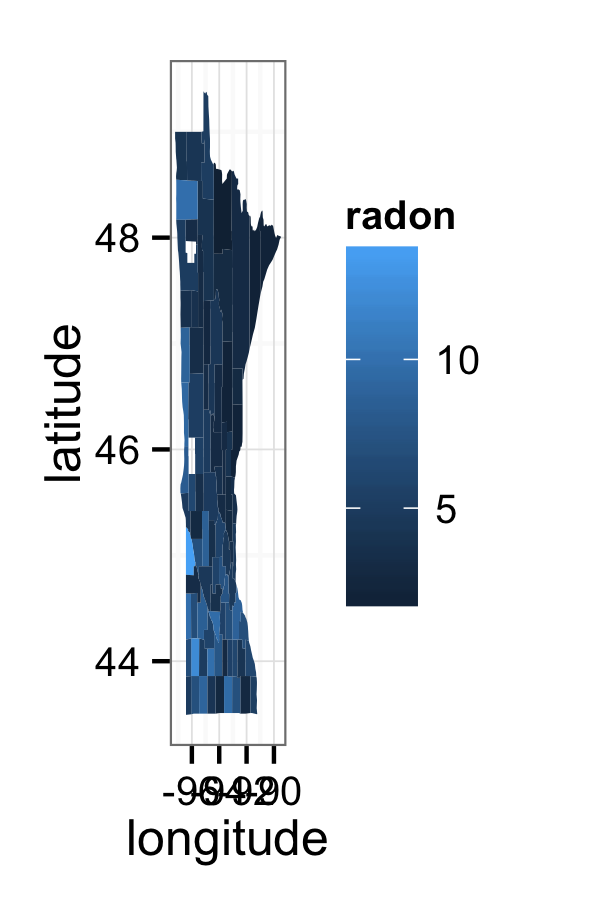
\includegraphics[width=0.5\textwidth]{figures/map.png}
\caption{\label{fig:map} Map of the counties in Minnesota. The color shading represents average Radon activity.}
\end{figure}
%
\begin{figure}[htb]
\centering
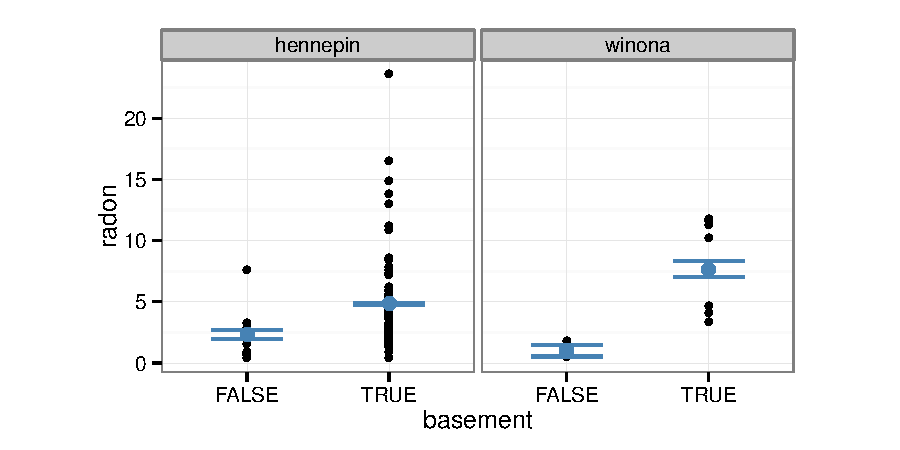
\includegraphics[width=0.7\linewidth]{figures/radon-twocounties.pdf}
\caption{\label{fig:tc} Activity of radon levels for Hennepin and Winona counties at basement \hh{(basement = TRUE) or higher in the residence}. The bigger points indicate the sample means with 95\% confidence intervals  given by the error bars. Radon levels at the basement level are usually higher.}
\end{figure}
%
The within-county sample sizes, $n_i$, are extremely unbalanced, ranging from one house to 116 houses, with 50\% of the counties having between three and ten houses. Such unbalanced designs are common in applications, and result in a high degree of pooling in the predicted random effects, which results in quantities for many counties that are highly shrunken toward the global mean. It is this high degree of shrinkage that leads to dependence between  predicted random effects and error terms (cf. eqns. \ref{eq:resid1} and \ref{eq:resid2}), which in turn can lead us to draw erroneous conclusions for corresponding residual quantities.

\begin{figure}[!h]
	\centering
	  \subfloat[Predicted error terms]{
		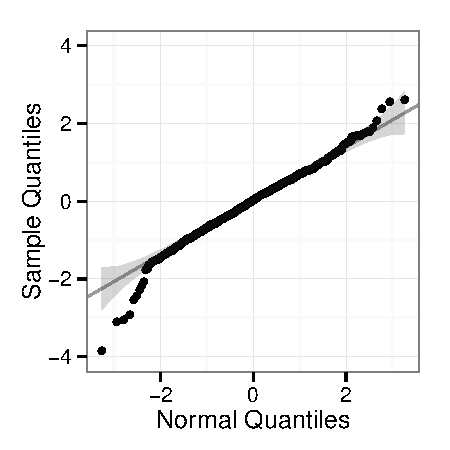
\includegraphics[width=0.33\linewidth]{raw-lev1-qq.pdf}
	   }
	  \subfloat[Random intercepts]{
		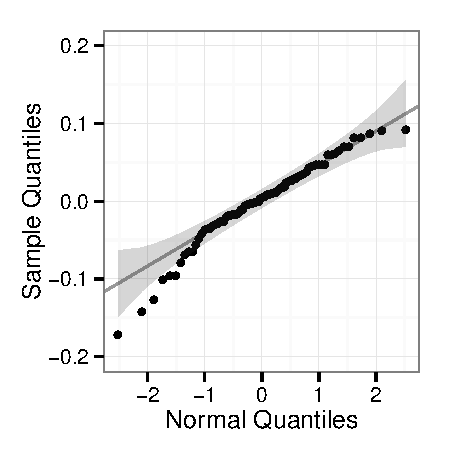
\includegraphics[width=0.33\linewidth]{raw-intercept-qq.pdf}
		}
%	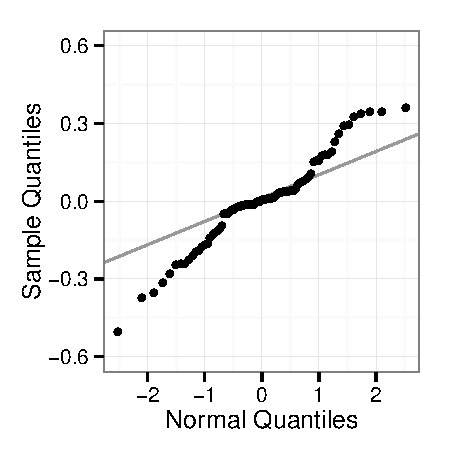
\includegraphics[width=0.32\textwidth]{raw-slope-qq.pdf}
	\caption{\label{fig:qqplots1} Q-Q plots of predict\al{ed residuals} at different levels %, and random slopes (right) 
	for model~\eqref{eq:radon}. \hh{Both plots suggest a deviation of residuals from a normal distribution.} Note that random slopes (see figure~\ref{fig:lineup}) exhibited the largest deviation from normality. }
\end{figure}

\begin{figure}[htb]
	\centering
	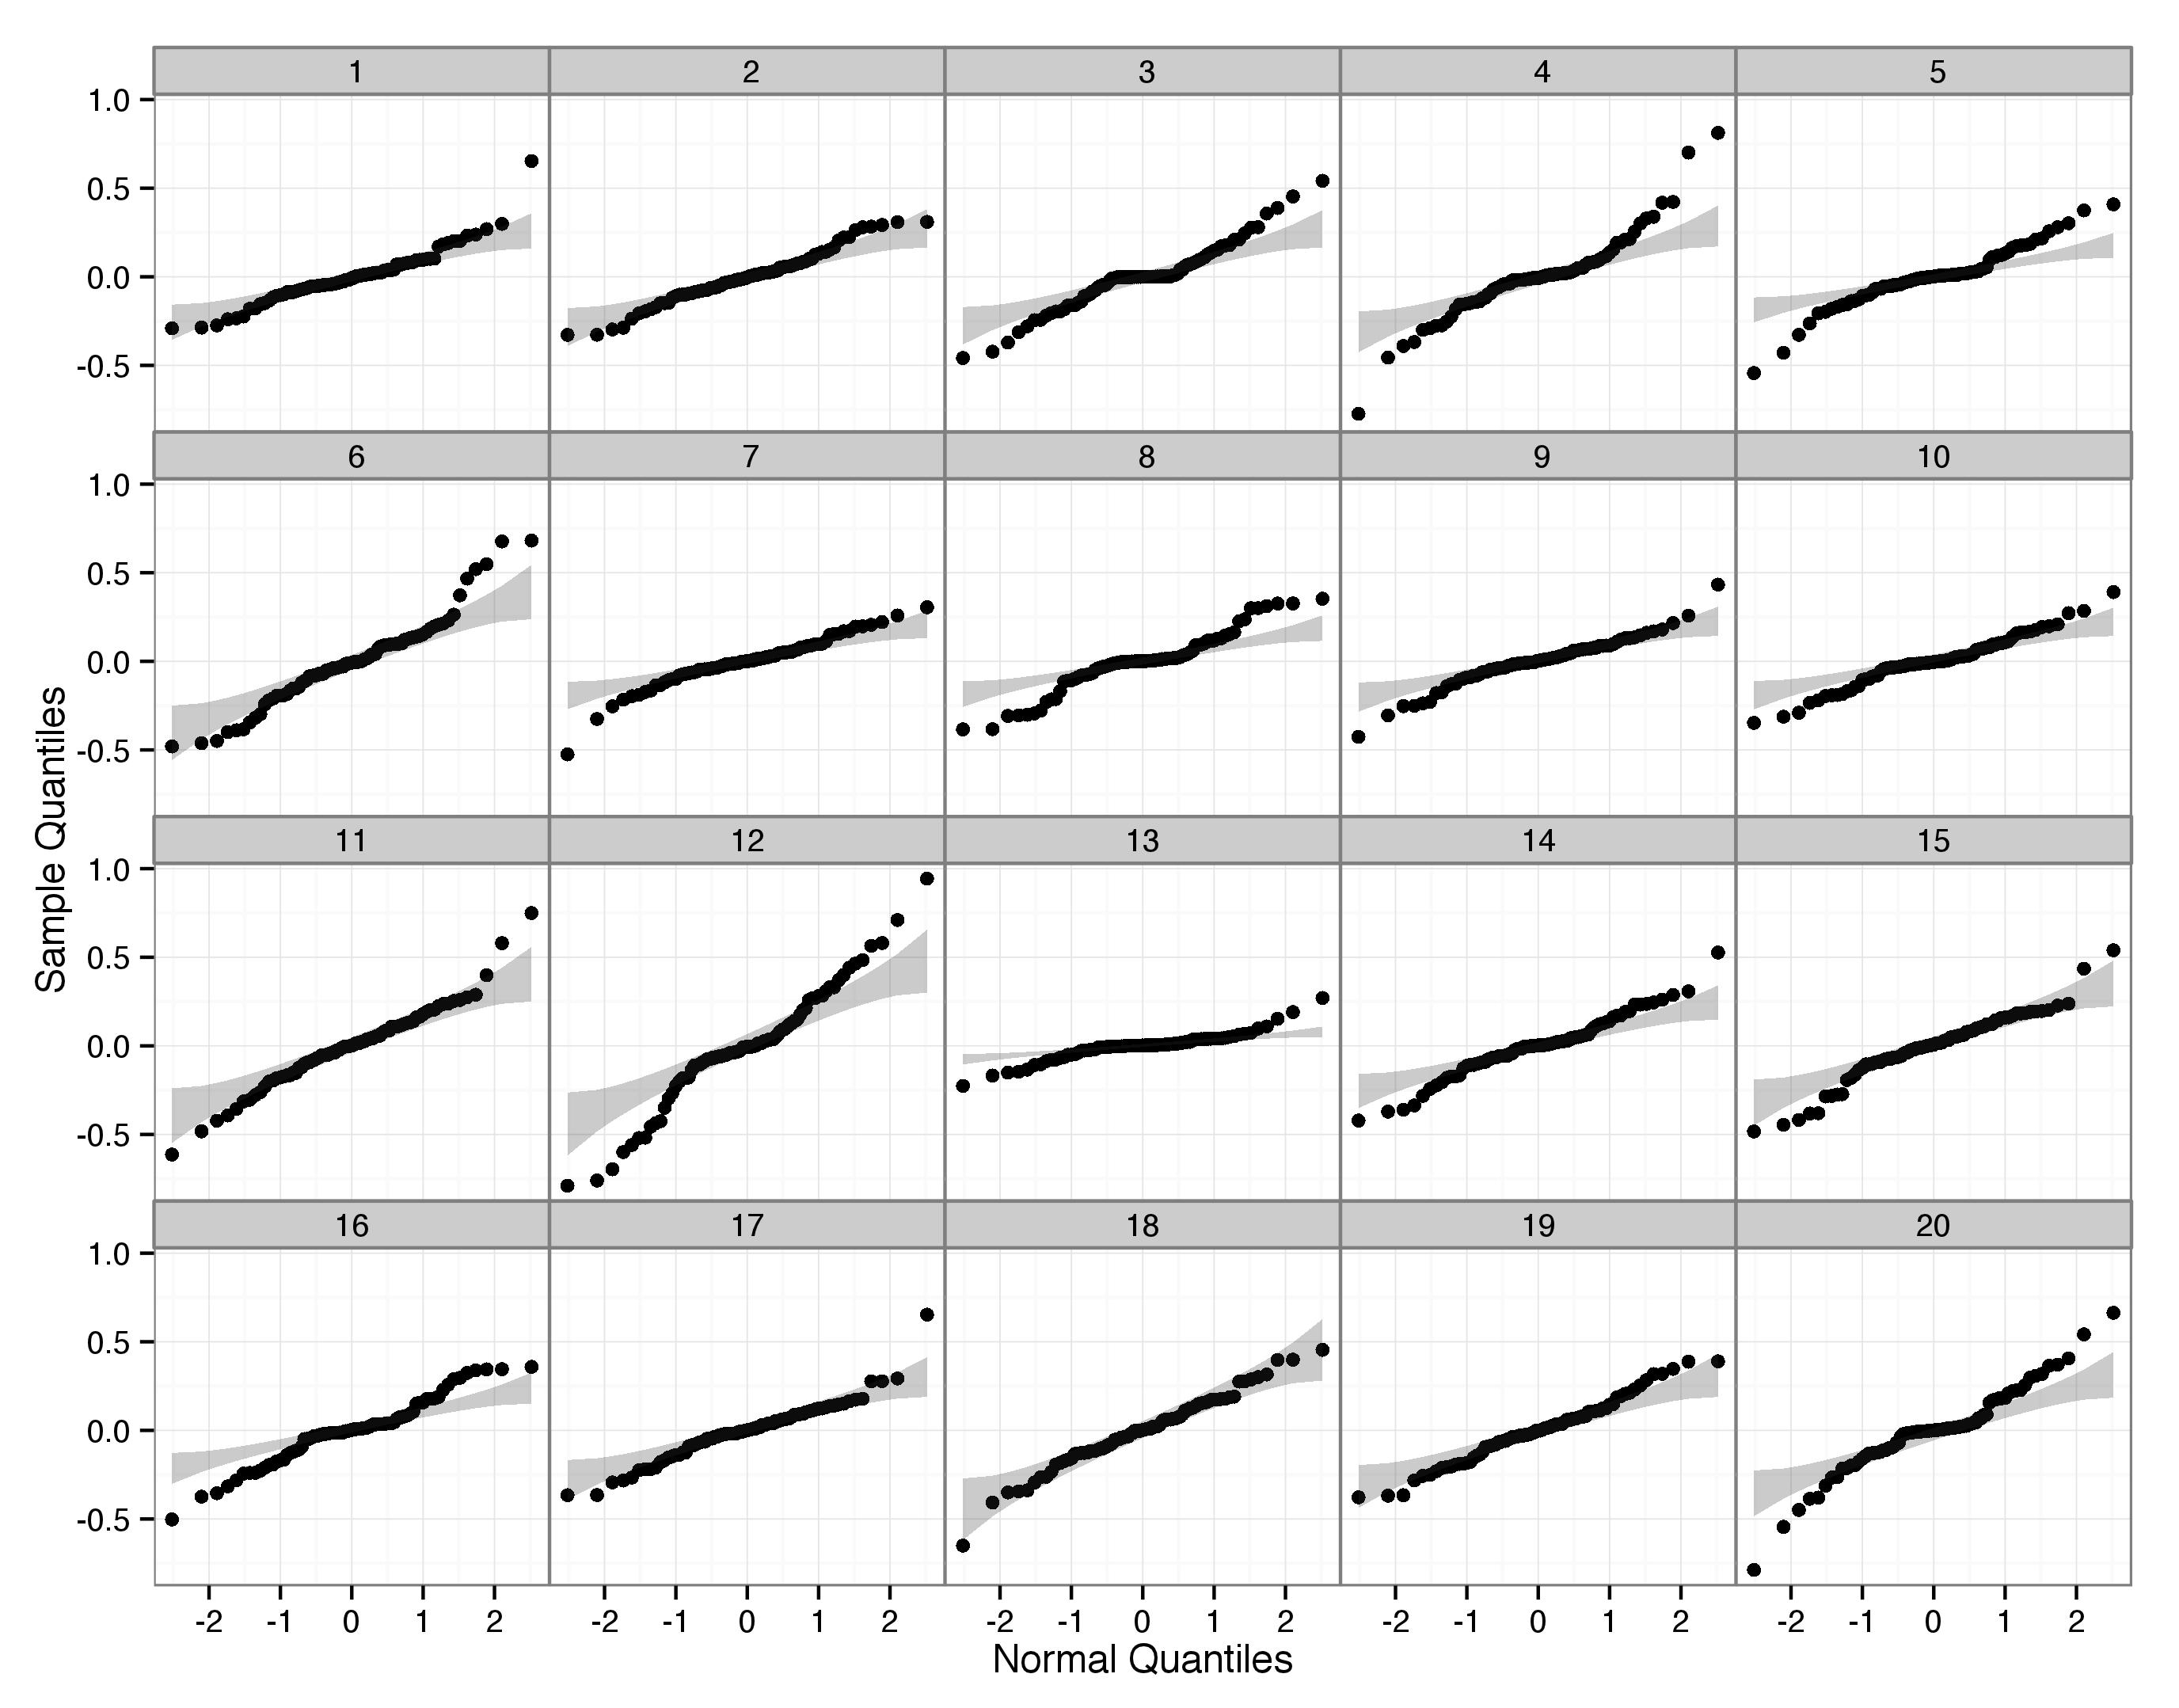
\includegraphics[width=0.9\textwidth]{test.jpeg}%lineup-rslope.pdf}
	\caption{\label{fig:lineup} Lineup of normal Q-Q plots for the random slope term in model~\eqref{eq:radon}. The 19 null plots were obtained by simulation from the model. Can you identify the observed Q-Q plot? }
\end{figure}


In this example, Q-Q plots (Figure~\ref{fig:qqplots1}) for the residuals show that normality 
seems to be violated for the error terms and both random effects. But is this cause for concern?
\al{As} there is little pooling at the observation level \al{(level 1)} we expect the distributional assessment of the error terms to be reliable, but  the high degree of pooling  for the random effects  casts doubt on the reliability of their Q-Q plots. 
 We find our doubts increasing in a simulation-based assessment of distributions for residuals and random effects. \hh{this sentence is a lead in to the next paragraph, right? It needs to that more explicitly.}

Figure~\ref{fig:lineup} shows a lineup \citep{buja:2009} of 20 Q-Q plots for the predicted random slope. The Q-Q plot of the observed random slopes is placed among 19 decoy plots of parametric bootstrap samples based on model~\eqref{eq:radon} satisfying the normal distribution assumptions. The simulation parameters were set to the maximum likelihood estimates of model~\eqref{eq:radon}. \hh{describe first what happens if we can distinguish the data.}
The observed Q-Q plot (panel $12+2^2$) is virtually indistinguishable from the field of null plots. This suggests that the predicted random slopes  from the data do not deviate significantly from model~\eqref{eq:radon}. 
%A lineup of the random intercepts revealed the same finding and was omitted for brevity. 
Note that in practice we must blind ourselves from the true plot for proper use of lineups. In order to not violate this, we did not show the Q-Q plot of random slopes earlier.
%
%application of the Anderson-Darling test results in the rejection of the null hypothesis of normality at the .05 significance level for the error terms and both random effects. As there is little pooling at the observation level we would expect the distributional assessment of the error terms to be reliable, but this is not the case with the random effects. 
%
%To further explore the distributional assumptions made on the random effects we create lineups \citep{buja:2009} of quantile plots were created by randomly inserting the true quantile plot for each term into a field of 19 plots generated under the null hypothesis of normality. A lineup for the random slopes is presented in Figure~\ref{fig:lineup}. The observed quantile plot (panel 16) is indistinguishable from the field of null plots, indicating that these predicted random slopes do not deviate from what would be expected under model~\eqref{eq:radon}, contradicting the results of the AD test. 

What becomes apparent from the lineup, is that, astonishingly, {\it none} of the null plots conform to normality. Further investigation  reveals  that a  proportion far above the nominal $\alpha=0.05$ level of random intercepts also fail the normality tests. \hh{same thing as before - this is supposed to be the lead in to the next sentence, but it seems to indicate that you recite a result that you have done and don't want to show, which makes it a bit cryptic as to what you are doing next.}


%Further evidence of the impact of this dependence is evident from a small scale simulation study. We used the design of the radon study to simulate 5000 data sets under model~\eqref{eq:radon} satisfying the assumptions discussed above. The simulation parameters were set to the maximum likelihood estimates of model~\eqref{eq:radon}. 
%%: $\widehat{\beta_0} = 1.46$, $\widehat{\beta_1} = -0.64$, $\widehat{\beta_2} = 0.77$, $\widehat{\sigma}_{\varepsilon} = 0.75$, $\widehat{\sigma}_{b_0} = 0.12$, $\widehat{\sigma}_{b_1} = 0.35$, and $\widehat{\rho} = 0.26$. 


Table~\ref{tab:edf} shows results from 1000 parametric bootstrap samples of model~\eqref{eq:radon} assuming normal random effects and level-1 residuals generated as normal ($\varepsilon_{ij}^* \sim \mathcal{N}(\bm{0},\ \sigma^2_\varepsilon)$), heavy tailed ($\varepsilon_{ij}^* \overset{iid}{\sim} (\sigma_{\varepsilon} / \sqrt{3})\, t_3$), and skewed ($\varepsilon_{ij}^* \overset{iid}{\sim} \sigma_{\varepsilon} \, \{ \text{Exp}(1) - 1 \}$).
For each simulated data set, we evaluated the assumption of normality for both the level-1 and -2 residuals using the Anderson-Darling (AD), Cram{\'e}r von Mises (CVM) and  Kolmogorov-Smirnov (KS) tests for normality.  
%Table~\ref{tab:edf} shows the proportions of the tests of the empirical distribution function rejecting the null hypothesis of normality at the .05 significance level. 
The type I error rates are hugely inflated for both random effects, making an assessment of normality based on the empirical distribution impossible. \hh{pick one of the numbers from the table and use it as an example.} Use of standardized random effects and \citetapos{Lange:1989uu} weighted Q-Q plot \hh{how can you test the weighted Q-Q plot?} reduce the type I errors to the nominal level when the level-1 residuals are normal, but the type I errors remain inflated for non-normal level-1 residuals. Similarly, when the random effects are not normal, simulations (not shown) revealed that the tests were  often unable to reject the null hypothesis of normality when the level-1 residuals were normal. \al{Based on the above results we find that distributional assessment of the predicted random effects is confounded by the distribution of the level-1 residuals.}
%The inflated type I error rates for the random effects indicate that the empirical distribution of the random effects cannot be used to assess the assumption of normality. 
In this example we are able to use the empirical distribution to assess normality of  level-1 residuals  as  pooling is minimal at this level. In situations with higher levels of pooling, this may not be the case.

\begin{table}[t]
\centering
\caption{\label{tab:edf} Proportion of tests rejecting the null hypothesis of normality of the predicted random effects at the nominal $\alpha=.05$ significance level when the error terms are normal, heavy tailed, and skewed. The proportions are hugely inflated under each setting compared to the nominal type I error rate. \vspace{.5em}}
\subfloat[Random intercept]{
	\begin{tabular}{l rrr} \hline
	& \multicolumn{3}{c}{Test} \\ \cline{2-4}
	  	&     AD & CVM  & KS \\ \hline
	Normal       	   &	 0.66 & 0.61 & 0.47  \\ 
	Heavy tailed 	   & 0.91 & 0.90 & 0.80  \\ 
	Skewed       	   & 0.85 & 0.82 & 0.71  \\  
	\hline
	\end{tabular}
}
\qquad
\subfloat[Random slope]{
	\begin{tabular}{l rrr} \hline
	& \multicolumn{3}{c}{Test} \\ \cline{2-4}
	  	&     AD & CVM  & KS \\ \hline
	Normal       	  & 0.74 & 0.71 & 0.59  \\ 
	Heavy tailed 	  &	0.94 & 0.94 & 0.87  \\ 
	Skewed       	  &	0.89 & 0.87 & 0.79  \\  
	\hline
	\end{tabular}
}


%\subfloat[Standardized Random intercept]{
%	\begin{tabular}{l rrr} \hline
%	& \multicolumn{3}{c}{Test} \\ \cline{2-4}
%	  	&     AD & CVM  & KS \\ \hline
%	Normal       	   &	 0.048 &	 0.045 &	 0.046  \\ 
%	Heavy tailed 	   & 0.349 & 0.325 & 0.256  \\ 
%	Skewed       	   & 0.520 & 0.487 & 0.399  \\  
%	\hline
%	\end{tabular}
%}
%\qquad
%\subfloat[Standardized Random slope]{
%	\begin{tabular}{l rrr} \hline
%	& \multicolumn{3}{c}{Test} \\ \cline{2-4}
%	  	&     AD & CVM  & KS \\ \hline
%	Normal       	  & 0.039 &	0.041 &	0.048  \\ 
%	Heavy tailed 	  &	0.434 & 0.403 & 0.320  \\ 
%	Skewed       	  &	0.540 & 0.504 & 0.422  \\  
%	\hline
%	\end{tabular}
%}

\end{table}


%\begin{table}[!h]
%\caption{\label{tab:edf} Proportions of tests rejecting the null hypothesis of normality of the predicted error terms and random effects at the nominal .05 significance level. \hh{didn't we want to keep the  background for power? - it should be consistent throughout the paper} Type I error rates are hugely inflated. \vspace{.5em}
%}
%\begin{center}
%\begin{tabular}{l rrr} \hline
%& \multicolumn{3}{c}{Test} \\ \cline{2-4}
% Residual &  AD & CVM & KS \\ \hline
%Error term			 & 0.06 & 0.06 & 0.05\\
%\rowcolor{gray!20} Random intercept 	& 0.48 & 0.46 & 0.35\\
%\rowcolor{gray!20} Random slope 		& 0.75 & 0.75 & 0.68\\
%   \hline
%\end{tabular}
%\end{center}
%\end{table}


In the remainder of this paper we investigate the root of concern that leads to the distributional deviations, and derive residuals that address the issues introduced by pooling, allowing again for a familiar graphical assessment of these distributions.

%----------------------------------------------------------------------------------
\section{Hierarchical linear models and residuals}\label{sec:resid}
%----------------------------------------------------------------------------------
\hh{What is the purpose of section 3? It doesn't stand on its own - move it as a subsection into section 4}


The general stacked representation of the hierarchical linear model is given by
%
\begin{eqnarray}\label{eq:hlm}
 && \bm{y} = \bm{X \beta} + \bm{Z b} + \bm{\varepsilon}, \\ \nonumber
 && \E \begin{bmatrix} \bm{b} \\ \bm{\varepsilon} \end{bmatrix} = \bm{0}, 
 \ \cov \begin{bmatrix} \bm{b} \\ \bm{\varepsilon} \end{bmatrix} = 
  	\begin{bmatrix} \bm{D} & \bm{0}\\ \bm{0} & \bm{R} \end{bmatrix}
\end{eqnarray}
%
where $\bm{y}$ is an $n \times 1$ vector of observed responses, $\bm{X}$ ($n \times p$) and $\bm{Z}$ ($n \times q$) are design matrices, $\bm{\beta}$ is a $p \times 1$ vector of unknown fixed effects, $\bm{b}$ is a $q \times 1$ vector of unobserved random effects, $\bm{\varepsilon}$ is an $n \times 1$ vector of unobserved errors, and $\bm{R}$ and $\bm{D}$ are positive definite covariance matrices.

  %Additionally, it is often assumed that $\bm{\varepsilon}$ and $\bm{b}$ are normally distributed. 
Using this specification, the predicted error terms and random effects are given by 
%
\begin{align}
\widehat{\bm{\varepsilon}} &= \bm{RPy} = \bm{RPZb} + \bm{RP \varepsilon} \label{eq:resid1}\\
\widehat{\bm{b}} &= \bm{DZ}\trans \bm{Py} = \bm{DZ}\trans \bm{PZb} + \bm{DZ}\trans \bm{P \varepsilon} \label{eq:resid2}
\end{align}
%
where $\bm{P} = \bm{V}\inv( \bm{I} - \bm{X} (\bm{X}\trans \bm{V}\inv \bm{X})\inv \bm{X}\trans \bm{V}\inv)$. This  set of equations %\eqref{eq:resid1} and \eqref{eq:resid2} 
reveals the inherent dependence between the residuals.
Additionally, it is easily seen that both \eqref{eq:resid1} and \eqref{eq:resid2} lead to the analysis of correlated and potentially heteroscedastic disturbances as $\var(\widehat{\bm{\varepsilon}}) = \bm{RPR}$ and $\var(\widehat{\bm{b}}) = \bm{DZ}\trans \bm{PZD}$.
The use of standardized residuals can correct the latter issue, but does not address the fact that the residuals are interrelated. While problems may be expected at both levels of the model based on \eqref{eq:resid1} and \eqref{eq:resid2}, we have found that the interpretation of Q-Q plots of the standardized predicted error terms
%
\[
\bm{z}_{\varepsilon} =  \text{diag} \left(\bm{RPR} \right)^{-1/2} \widehat{\bm{\varepsilon}}
\]
%
is unaffected by this interrelationship; however, this is not the case with the standardized random effects.  When the degree of pooling is high---as it is in the above radon example, and often is in practice---interpretation of the predicted random effects cannot be separated from the distribution of the error terms. Detailed simulation results documenting the utility of  these residuals are available in the supplementary material.



%----------------------------------------------------------------------------------
\section{Rotating the random effects}\label{sec:rotate}
%----------------------------------------------------------------------------------

To combat \al{the confounded nature of the predicted random effects}, we derive a reduced set of rotated residuals that are standardized, uncorrelated, and homoscedastic. \al{We focus our discussion (and notation) on a two-level model with a single random effect in this section for ease of explanation, and describe how to extend this method at the end of this section.} \cite{HildenMinton:1995wh} presents the derivation of a similar set of residuals for the error terms, but does not address the random effects which are the focus of this paper. 

First, we define the \emph{fraction of confounding} for the random effects, which is minimized in the result below. This definition generalizes the fraction of confounding proposed by \cite{HildenMinton:1995wh}. \\

%\begin{definition}[Fraction of confounding]\label{def:fc1}
%For the $i$th element of the target residual vector, $\widehat{\bm{e}}$, the fraction of confounding is given by
%%
%\begin{equation}\label{eq:fc}
%	\text{FC}(\widehat{\bm{e}}_i) 
%	= \frac{\bm{v_i}\trans \var(\widehat{\bm{e}} | \bm{e}) \bm{v_i}}
%		{\bm{v_i}\trans \var(\widehat{\bm{e}}) \bm{v_i}}
%	= \frac{\bm{v_i}\trans \bm{A} \bm{v_i}}
%		{\bm{v_i}\trans \bm{B} \bm{v_i}}
%\end{equation}
%
%where $\bm{v_i}$ is the $i$th column of the identity matrix.
%%\todo[inline]{write this as a minimization problem}
%%This rotation is given by $\bm{M} = \bm{T_r \Lambda_r}^{-1/2} \bm{U}$ where $\bm{T_r \Lambda_r}^{-1/2}$ is the inverse square root of $\bm{B}$ found through the spectral decomposition of $\bm{B}$ and $\bm{U}$ are the eigenvectors of $(\bm{\Lambda_r}^{-1/2} \bm{T_r}\trans) \bm{A} (\bm{\Lambda_r}^{-1/2} \bm{T_r}\trans)\trans$.
%\end{definition}

%Definition~\ref{def:fc1} describes the confounding for each element in the target residual vector individually. An overall measure of the amount of confounding is given below.\\

%\begin{definition}\label{defc:fc2}
%For the target residual vector, $\widehat{\bm{e}}$, the fraction of confounding is given by
%%
%\begin{equation}\label{eq:fc2}
%FC(\widehat{\bm{e}}) = \mathrm{tr}( \var(\widehat{\bm{e}} | \bm{e} ) ) / \mathrm{tr}( \var(\widehat{\bm{e}}) ).
%\end{equation}
%\end{definition}

\begin{definition}[Fraction of confounding]
Let $\bm{A} = \var(\widehat{\bm{b}} | \bm{b} )$ and $\bm{B} = \var(\widehat{\bm{b}})$, which are positive semidefinite matrices by definition, then the fraction of confounding in $\widehat{\bm{b}}$ is given by
%
\begin{equation}\label{eq:fc2}
\text{FC}(\widehat{\bm{b}}) = \frac{1}{\ell} \tr\left( \bm{B}\ginv\bm{A} \right)
%\dfrac{1}{\ell} \displaystyle{\sum_i} \frac{\bm{v_i}\trans \bm{A} \bm{v_i}}
%		{\bm{v_i}\trans \bm{B} \bm{v_i}}.
\end{equation}
where $\ell$ is the length of vector $\widehat{\bm{b}}$.
\end{definition}
The fraction of confounding measures the contribution of the error terms  to the variance of the random effects. $\text{FC} \in [0,1]$, where 1 indicates that, due to confounding, the predicted random effects contain no information in addition to that found in the error terms, while 0 indicates no confounding. 


In order to correct residuals for the impact of confounding, we propose using a linear transformation of the random effects, $\bm{W}^{*\prime} \widehat{\bm{b}}$, that projects the random effects into $s$-dimensional space and satisfies
%find weights $\bm{w_i}$ to apply to each of the residual contributions that minimize $\tr\left( \bm{B}\ginv\bm{A} \right)$. This can be re-expressed as the following minimization problem:
%\[
%\bm{w}_{\ell-r} = \arg \min_{w \neq 0} \frac{\bm{w}\trans \bm{A} \bm{w}}
%		{\bm{w}\trans \bm{B} \bm{w}}.
%\]
\begin{equation}\label{eq:minimize}
\bm{W}^* = \argmin_{W \in \mathbb{R}^{\ell \times s} } 
\tr\left( \left(\bm{W\trans B W} \right)\inv \left(\bm{W\trans A W}\right) \right)
%\displaystyle{\sum_i} \frac{\bm{v_i}\trans \bm{W} \bm{A} \bm{W}\trans \bm{v_i}}
%		{\bm{v_i}\trans \bm{W} \bm{B} \bm{W}\trans \bm{v_i}}
\end{equation}
%where $\ell$ is the length of vector $\bm{b}$. %and $r = \text{rank}(\bm{B})$. 
\al{This problem is solved using the generalized eigenvalue decomposition
\begin{equation}\label{eq:geigen}
	\bm{Aw}_k = \gamma_k \bm{Bw}_k
\end{equation}
where $\gamma_k$ and $\bm{w}_k$ are the $k$-th smallest eigenvalues and eigenvectors, respectively \citep{Fukunaga:1990}; thus, $\bm{W}^*$ consists of the eigenvectors associated with the $s$ smallest eigenvalues. Computationally, this problem can be solved by simultaneous diagonalization of $\bm{A}$ and $\bm{B}$. We outline this procedure below for reference and refer the reader to \cite{McDonald:1979ca} and \cite{deLeeuw:1982to} for additional details on simultaneous diagonalization of two positive semidefinite matrices.\\}

\begin{algorithm}[Simultaneous diagonalization]
Let $\bm{A}$ and $\bm{B}$ be two positive semidefinite matrices. The transformation that simultaneously diagonalizes both matrices can be found through the following procedure:
\begin{enumerate}
\item Find a transformation that whitens $\bm{B}$. Such a transformation is given by $\bm{T_r \Lambda_r}^{-1/2}$, where $\bm{T}_r$ and $\bm{\Lambda}_r$ are the first $r$  eigenvectors and eigenvalues of $\bm{B}$, where $r = \rank(\bm{B})$. 

\item Transform $\bm{A}$ and $\bm{B}$ to
\begin{align}
\bm{\Lambda_r}^{-1/2} \bm{T_r}\trans \bm{A T_r \Lambda_r}^{-1/2} &= \bm{A}^* \label{eq:astar} \\
\bm{\Lambda_r}^{-1/2} \bm{T_r}\trans \bm{B T_r \Lambda_r}^{-1/2} &= \bm{I}
\end{align}

\item Find an orthonormal transformation that diagonalizes $\bm{A}^*$. Such a transformation is given by the eigenvectors of $\bm{A}^*$, which we denote $\bm{U}$.
\end{enumerate}

Based on the above three steps, the transformation that simultaneously diagonalizes $\bm{A}$ and $\bm{B}$ is $\bm{T_r \Lambda_r}^{-1/2} \bm{U}$.\\ 

\end{algorithm}

The above procedure can be used to find the general solution to \eqref{eq:geigen}. To find the more specific transformation $\bm{W}^*$ that projects the random effects into an $s$-dimensional space satisfying \eqref{eq:minimize}, we focus on the $s$ eigenvectors associated with $s$ the smallest eigenvalues of $\bm{A}^*$, $\bm{U}_s$, making
%
\begin{equation}\label{eq:w}
\bm{W}^* = \bm{T_r \Lambda_r}^{-1/2} \bm{U}_s
\end{equation}
%
The rotated random effects are then given by $\bm{W}^{*\prime} \widehat{\bm{b}}$, which are standardized, uncorrelated, and homoscedastic (see the appendix for a proof).

%\todo[inline]{Address that the order of the data will influence the resulting residuals.}
%Since $\bm{B}$ is only positive semidefinite, it is important to note that the order of the groups in the data change the resulting residuals. In this case, the transformation in \eqref{eq:astar} eliminates a group


Having considered the computational aspects of the problem we must next consider the more practical aspects. 

\hh{Rather than referring to $s$ give it a name and refer to that - `dimension of the subspace' maybe?}
\paragraph{Selecting $s$.}
First, we must consider the selection of $s$,  the length of the resulting transformed residual vector. One choice is $s = \rank(\bm{B})$, which aligns with the suggestion given by \cite{HildenMinton:1995wh} for the level-1 residuals. 
%This selection has the advantage that it works in all situations, but the disadvantage that the fraction of confounding will \al{often} not be \al{significantly} reduced. 
An alternative approach is to select $s$ based on the desired reduction in the fraction of confounding. 
%A starting point for this approach can be determined for a given reduction in the fraction of confounding by considering the relative contributions of the ordered diagonal elements of $\bm{B}\ginv\bm{A}$ to \eqref{eq:fc2}. 
We consider this approach in the simulation study presented in Section~\ref{sec:simulation} and present the results in Figure~\ref{fig:fc}. Note that in some situations it will not be possible to reduce the fraction of confounding much as the number of groups limits this reduction.

\paragraph{Correcting for supernormality.}
The transformation of the random effects results in a vector where each component is a linear combination of elements of $\widehat{\bm{b}}$. Consequently, the rotated residuals will appear more normal than the underlying distribution, if the underlying distribution is not normal. This issue is often referred to as supernormality \citep{Atkinson:1985}. One approach to address supernormality in this context is to reduce the number of elements in the linear combinations, which should reduce the extent of the problem. To do this, we suggest using an orthogonal rotation of $\bm{W}^*$, which we denote $\bm{Q}$, just as we rotate the factor loadings in factor analysis. Using this approach, the rotated residuals are obtained by $\bm{Q}\trans \bm{W}^{*\prime} \widehat{\bm{b}}$. One rotation that will produce rotated residuals comprised of a small number of raw residuals is the varimax rotation \citep{Johnson:2007}. Figure~\ref{fig:cartoon} displays heatmaps of $\bm{W}^{*\prime}$ (left) and $\bm{Q}\trans\bm{W}^{*\prime}$ (right) for a simulated random intercept model with 20 groups, and demonstrates that the varimax rotation reduces the number of groups loading highly on each rotated residual.  Other orthogonal rotations could be used, but the varimax rotation is familiar to a wide range of analysts and is widely implemented in statistical software packages. A similar approach was used by \cite{Jensen:1999iu}, who used the raw varimax rotation to produce recovered errors for distributional assessment in the ordinary regression model.

\begin{figure}[t]
	\centering
	\subfloat[$\bm{W}^{*\prime}$]{
		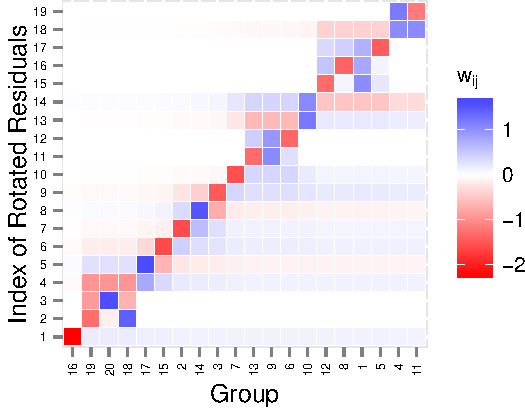
\includegraphics[width=0.4\textwidth]{cropped_cartoon_heatmap_raw.pdf}
	}
	\qquad
	\subfloat[$\bm{Q}\trans\bm{W}^{*\prime}$]{
		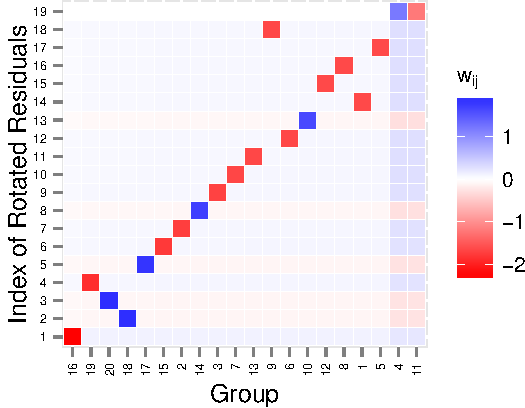
\includegraphics[width=0.4\textwidth]{cropped_cartoon_heatmap_varimax.pdf}
	}
	\caption{\label{fig:cartoon} Heatmap of $\bm{W}^{*\prime}$ and $\bm{Q}\trans\bm{W}^{*\prime}$ calculated where $\bm{Q}$ for a simulated random intercept model with 20 groups. Applying the varimax rotation, $\bm{Q}$, reduces the number of groups loading on a given rotated residual.}
\end{figure}

\paragraph{Extension to multiple random effects.}
Up to this point our discussion has ignored that a model may (and often will) contain numerous random effects. In this case, the assumptions made on each random effect should be checked; thus, we propose assessing each random effect separately. To this end we must define linear combinations $\bm{L}_k$ such that $\bm{L}_k\trans \widehat{\bm{b}}$ produces the $k$th marginal random effect. For example, in a model with a random intercept and random slope, if $\bm{Z}$ is organized as a block diagonal matrix---that is $\bm{Z} = \bigoplus_{i=1}^{m} \bm{Z}_{i}$ where $\bigoplus$ denotes the direct sum \citep[page 47]{Gentle:2007}---then $\bm{L}_0 = \bm{I}_{m} \bigotimes ( 1,\ 0)$ produces the random intercepts and $\bm{L}_1 = \bm{I}_{m} \bigotimes ( 0,\ 1)$ produces the random slopes. The methodology presented in this section can be generalized to models with numerous random effects by substituting $\bm{L}_k\trans \widehat{\bm{b}}$ for $\widehat{\bm{b}}$.


%----------------------------------------------------------------------------------
\section{Simulation study}\label{sec:simulation}
%----------------------------------------------------------------------------------

We conducted a simulation study to assess the specificity and sensitivity of tests of normality based on the two rotated residuals proposed in the previous section. 

\subsection{Design}\label{sec:sim-design}
%----------------------------------------------------------------------------------

The simulation study examined the proportion of Anderson-Darling (AD), Cram{\'e}r von Mises (CVM), and Kolmogorov-Smirnov (KS) tests that rejected the null hypothesis of normality. This allows us to examine situations in which we correctly and incorrectly reject the null hypothesis of normality---that is, power and type I error, respectively.  These test statistics each measure the discrepancy between the empirical distribution of the rotated random effects and assumed distribution of the random effects, which sheds light on the behavior of Q-Q plots constructed from the rotated residuals. 

The design matrices from model \eqref{eq:radon} were used as templates for realistic data generation; however, only the 60 counties with full rank $\bm{Z}$ matrices were included for simplicity of the simulation design.
The following distributions were used to generate simulated residuals $\varepsilon_{ij}^*$, $b_{0i}^*$, and $b_{1i}^*$ from which data were generated:
%
\begin{itemize}
\item $\varepsilon_{ij}^* \overset{iid}{\sim} \mathcal{N}(0, \ \sigma^2_{\varepsilon})$, or $\varepsilon_{ij}^* \overset{iid}{\sim} (\sigma_{\varepsilon} / \sqrt{3})\, t_3$ , or $\varepsilon_{ij}^* \overset{iid}{\sim} \sigma_{\varepsilon} \, \{ \text{Exp}(1) - 1 \}$

\item $b_{0i}^* \overset{iid}{\sim} \mathcal{N}(0, \ \sigma^2_{b_{0}})$, or $b_{0i}^* \overset{iid}{\sim} (\sigma_{b_{0}} / \sqrt{3})\, t_3$ , or $b_{0i}^* \overset{iid}{\sim} \sigma_{b_{0}} \, \{ \text{Exp}(1) - 1 \}$

\item $b_{1i}^* \overset{iid}{\sim} \mathcal{N}(0, \ \sigma^2_{b_{1}})$, or $b_{1i}^* \overset{iid}{\sim} (\sigma_{b_{1}} / \sqrt{3})\, t_3$ , or $b_{1i}^* \overset{iid}{\sim} \sigma_{b_{1}} \, \{ \text{Exp}(1) - 1 \}$
\end{itemize}
%
For simplicity we required the distributions of the random slope and intercept to the be same and assumed independence between the random effects. Additionally, the the fixed effects coefficients were set to the maximum likelihood estimates.

To investigate the effect that pooling has on the rotated random effects we considered  three variance structures:
%
\begin{itemize}
\item $\sigma^2_\varepsilon = 4$ and  $\sigma^2_{b_0} = \sigma^2_{b_1} = 1$
\item $\sigma^2_\varepsilon = 1$ and  $\sigma^2_{b_0} = \sigma^2_{b_1} = 1$
\item $\sigma^2_\varepsilon = 1$ and  $\sigma^2_{b_0} = \sigma^2_{b_1} = 4$

\end{itemize}
%

Under each simulation setting 1000 data sets were generated for each model and the rotated residuals were obtained using $s = \rank(\bm{B})$ (which are 58 and 59 for the random intercept and slope, respectively) as well as $s =$ 55, 50, 45, 40, 35, and 30.


\subsection{Results}\label{sec:sim-results}
%----------------------------------------------------------------------------------

Figure~\ref{fig:fc} shows the average fraction of confounding for the rotated random intercept (left) and random slope (right) over the different values for $s$ for each variance structure. As $s$ is reduced, the fraction of confounding is reduced, which aligns with expectation as smaller choices of $s$ reduce the contributions of more highly confounded groups.

\begin{figure}[h]
	\centering
	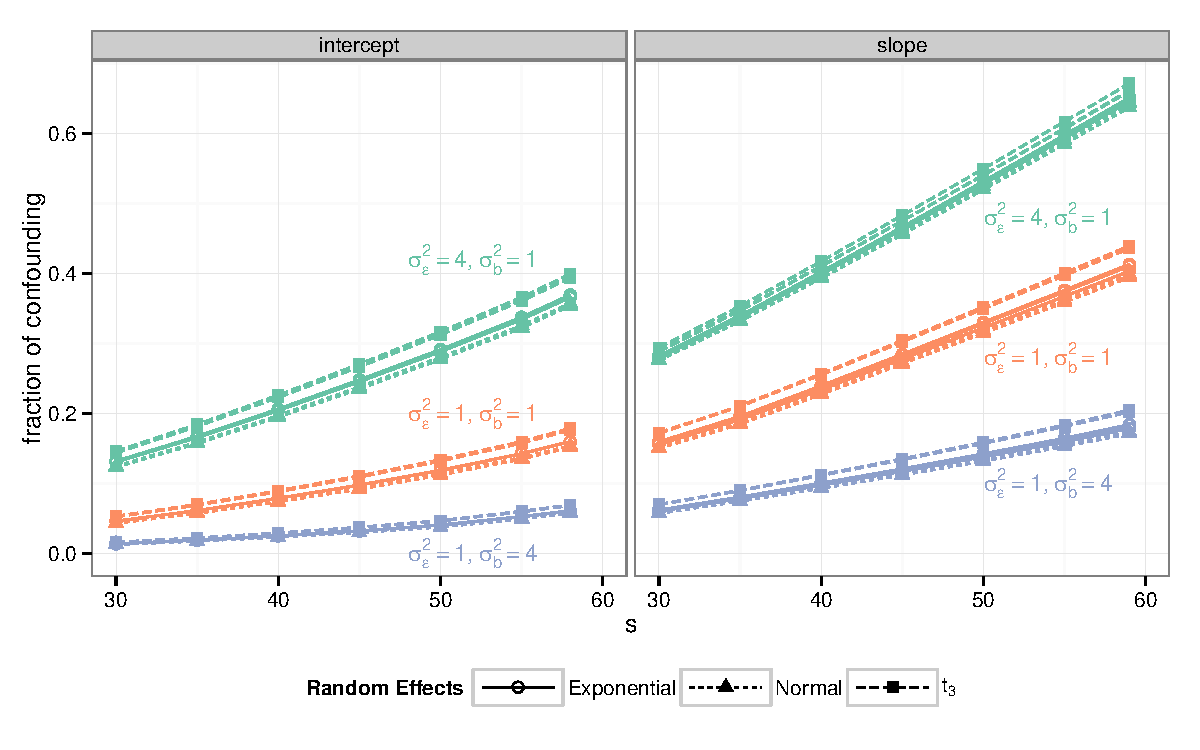
\includegraphics[width=\textwidth]{fc_by_s.pdf}
	\caption{\label{fig:fc} Change in the fraction of confounding (FC) as the dimension of the rotated random effects vector, $s$, is reduced for the three variance structures considered in the simulation study. %LOESS smoothers estimate the trajectory of FC as $s$ varies.} 
	\hh{Adam, I am not sure what b density is - could you fix that?}
	}
\end{figure}

Figures~\ref{fig:results-int} and \ref{fig:results-slope} display the estimated type I error rates using the AD normality test ($\alpha = 0.05$) on the rotated and varimax rotated random intercepts and random slopes when $\sigma^2_\varepsilon = 4$ and $\sigma^2_{b_0} = \sigma^2_{b_1} = 1$. The other tests performed similarly, and full simulation results can be found in the supplementary material. Both figures show that the type I error rate is stabilized close to the nominal level with the appropriate choice of $s$. For the random intercept most choices of $s$ perform reasonably well, with the type I error rate closest to the nominal level for all error distributions between 30 and 40. For the random slope, $s$ must be chosen to be 30 for type I error to be near the nominal level; however, $s$ may need to be even smaller to achieve the nominal rate. 

\begin{figure}
	\centering
	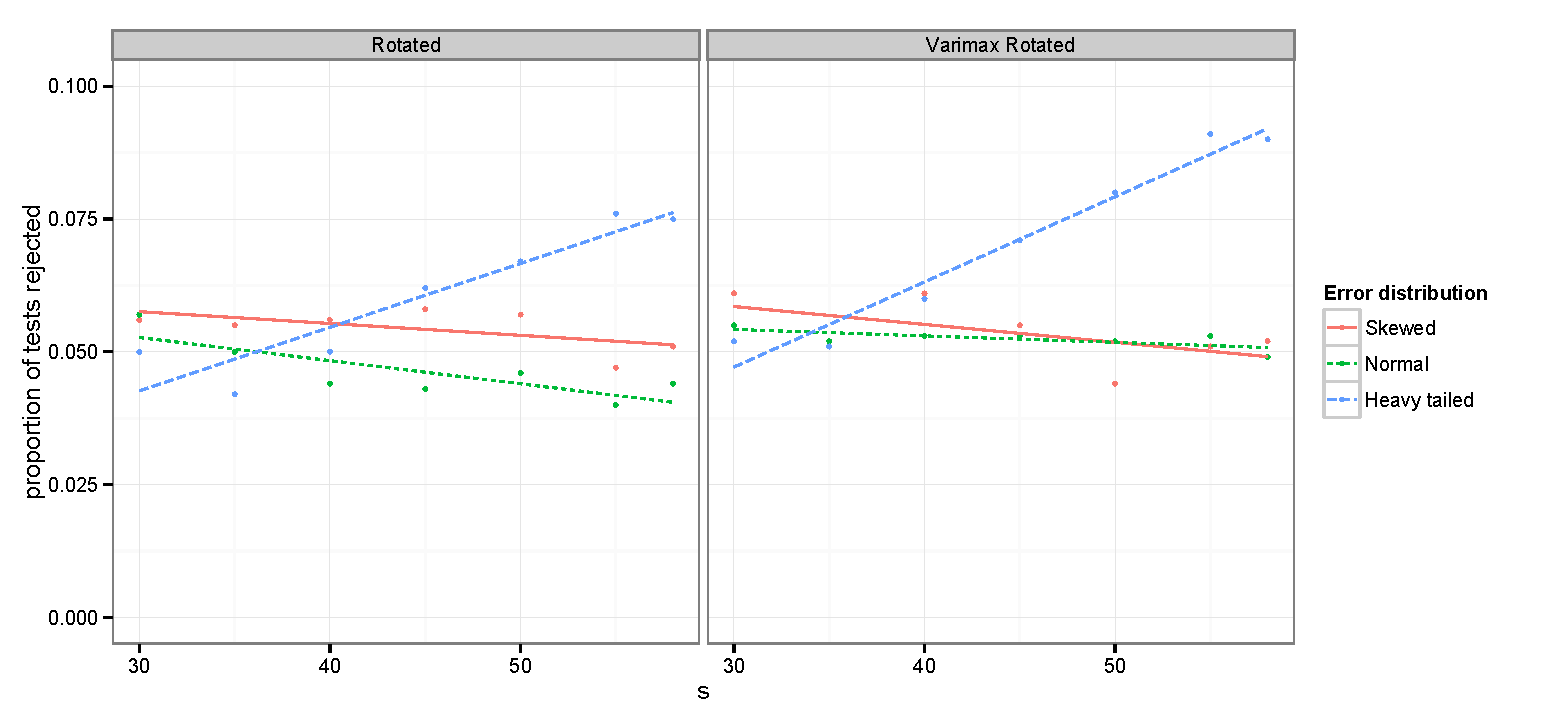
\includegraphics[width=\textwidth]{ad_intercept_results.pdf}
	\caption{\label{fig:results-int} Estimated type I error rate using the Anderson-Darling normality test ($\alpha = 0.05$) on the rotated random intercepts (left) and varimax rotated random intercepts (right) by the distribution of the error terms and $s$. }
\end{figure}

\begin{figure}
	\centering
	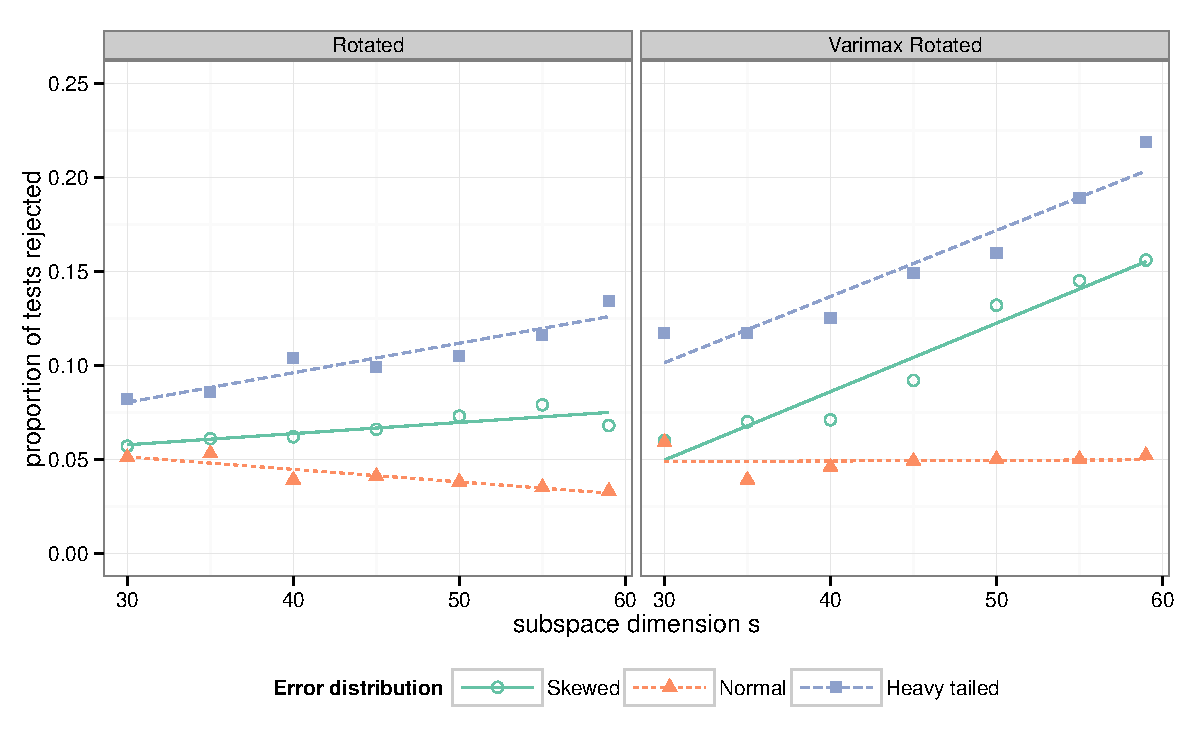
\includegraphics[width=\textwidth]{ad_slope_results.pdf}
	\caption{\label{fig:results-slope} Estimated type I error rate using the Anderson-Darling normality test ($\alpha = 0.05$) on the rotated random slopes (left) and varimax rotated random slopes (right) by the distribution of the error terms and $s$.}
\end{figure}

Figures~\ref{fig:power-int} and \ref{fig:power-slope} show the estimated power of the AD test ($\alpha = 0.05$) on the rotated and varimax rotated random intercepts and random slopes for the variance structure identified above. We find the estimated power to detect non-normal random effects distributions is amplified by the varimax rotation and larger choices of $s$. We also find that the estimated power is lower than would be expected from randomly sampled values from an exponential or $t_3$ distribution (what we will refer to as the ``gold standard''). For example, when $s=30$, simulations indicate the power of the AD test to detect a $t_3$ distribution to be approximately 0.4, whereas our simulations indicate nearly half the power, with the random slope generally having lower power than the random intercept. Interestingly, the there is higher power to detect a heavy tailed distribution than a skewed distribution.  Additional simulations (not discussed) using a model with a continuous variable defining the random slope showed results similar to the random intercept (Figure~\ref{fig:power-int}).

While the estimated power is lower than the gold standard, the fact that the type I error rate can be stabilized indicates that distributional problems detected using the rotated random effects will truly be problems; thus, providing more diagnostic information than the (unrotated) predicted random effects.

\begin{figure}
	\centering
	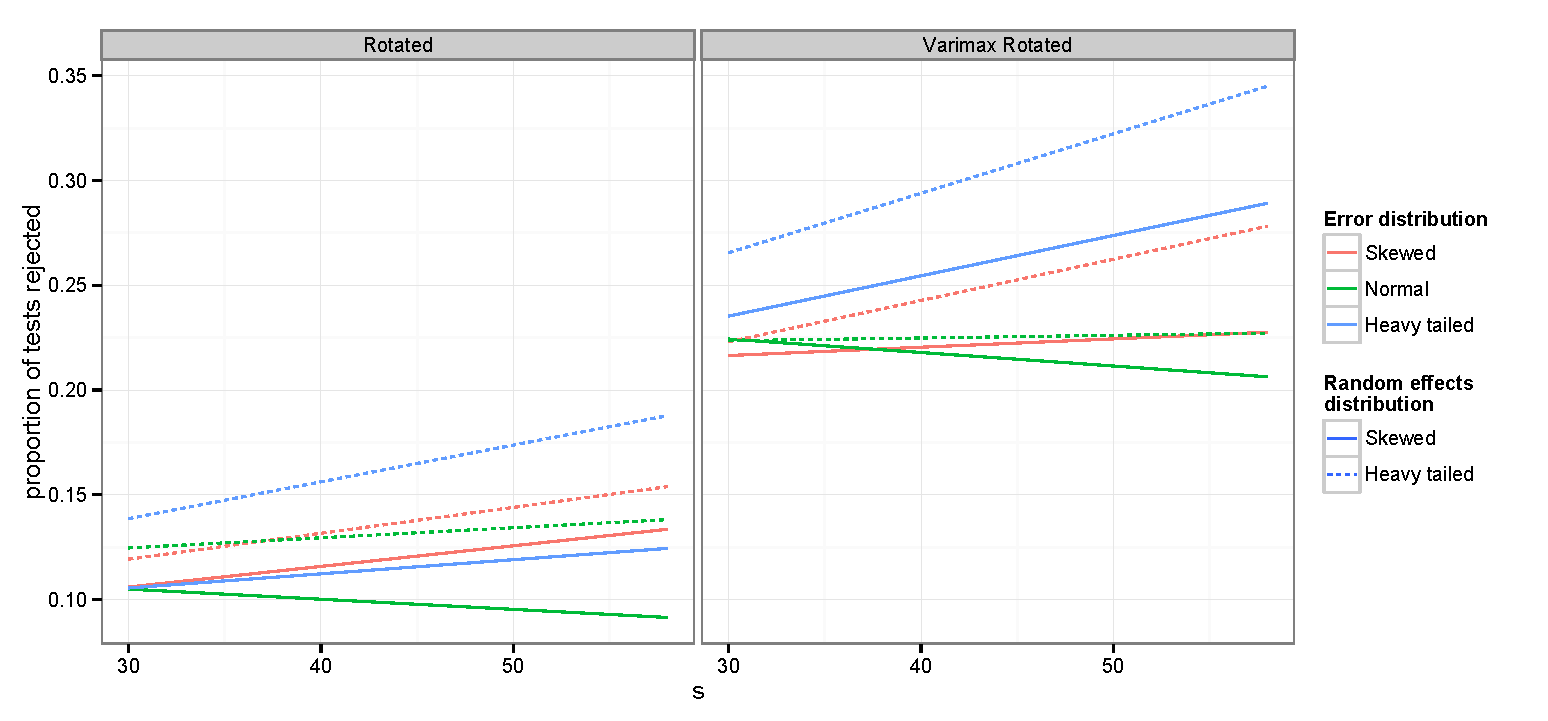
\includegraphics[width=\textwidth]{ad_intercept_power.pdf}
	\caption{\label{fig:power-int} Linear smoother of the estimated power using the Anderson-Darling normality test ($\alpha = 0.05$) on the rotated random intercepts (left) and varimax rotated random intercepts (right) by $s$. The color denotes the distribution of the errors and the linetype denotes the distribution of the random intercept.}
\end{figure}

\begin{figure}
	\centering
	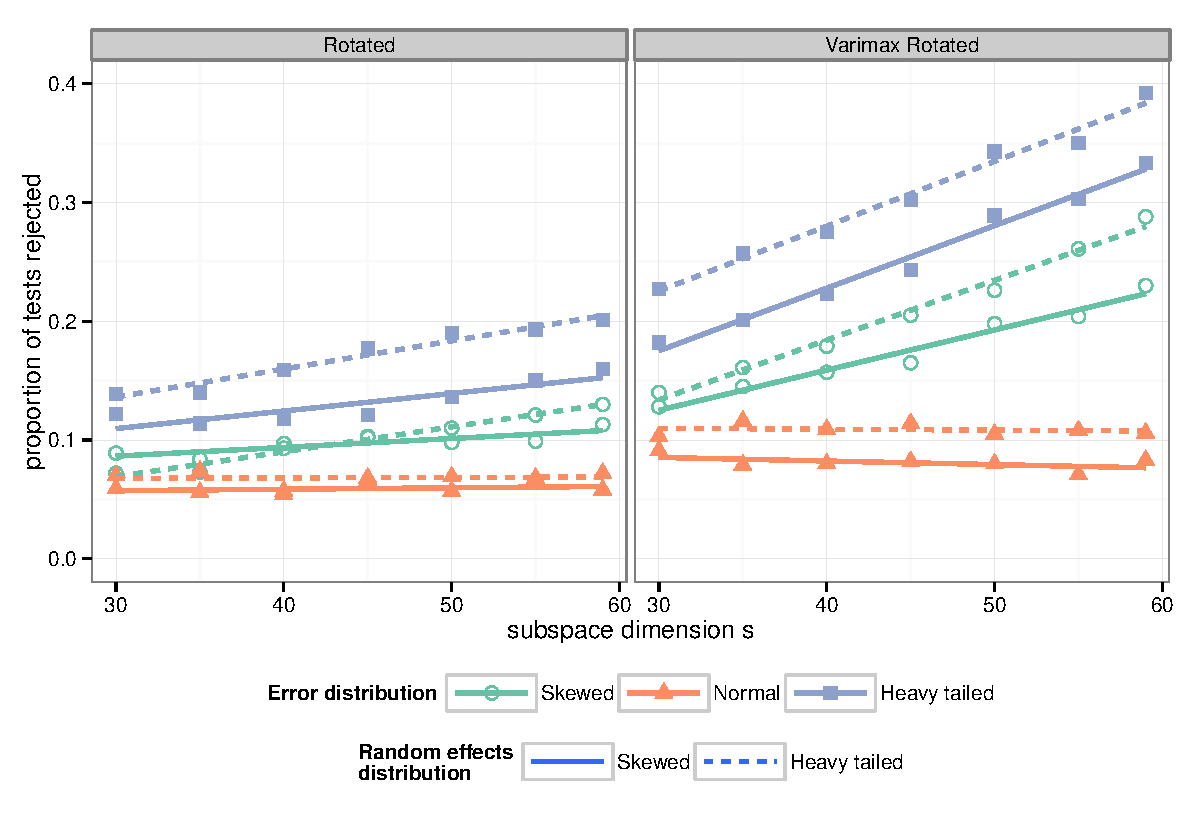
\includegraphics[width=\textwidth]{ad_slope_power.pdf}
	\caption{\label{fig:power-slope}Linear smoother of the estimated power using the Anderson-Darling normality test ($\alpha = 0.05$) on the rotated random slopes (left) and varimax rotated random slopes (right) by $s$. The color denotes the distribution of the errors and the linetype denotes the distribution of the random slope.}
\end{figure}



%\begin{itemize}
%\item Overall, the rotated residuals reduce the type I error rates to rates much closer to the nominal level. When $\sigma^2_\varepsilon > \sigma^2_b$ there is minor inflation of the type I errors when the error terms are non-normal, but less severe than without the rotation. When $\sigma^2_\varepsilon \leq \sigma^2_b$ the type I errors are essentially at the nominal levels.
%
%\item As expected, the power to detect non-normal random effects distributions is quite low for the rotated residuals. The varimax rotation does help amplify the power of detection, though an increase in the type I error rate also results.
%
%\item The power to detect non-normal random effects distributions increases as $\sigma^2_b$ increases relative to $\sigma^2_\varepsilon$.
%
%
%\end{itemize}

%----------------------------------------------------------------------------------
\section{Radon data: Revisited}\label{sec:radon2}
%----------------------------------------------------------------------------------
Next, we return to the motivating example and use rotated residuals to assess the distribution of the random effects using the rotated random effects. 
Recall that in Section~\ref{sec:ex} we determined that the error terms were not normally distributed. Consequently, examination of Q-Q plots of the predicted random effects will likely lead to erroneous conclusions due to the high degree of shrinkage. 

In order to construct Q-Q plots of the rotated random effects we first consider the choice of $s$. For model \eqref{eq:radon} the high degree of shrinkage leads to a large fraction of confounding for each random term: 0.72 for the random intercept and 0.70 for the random slope. In choosing $s$ we wish to reduce the fraction of confounding to approximately 0.5, but we will restrict attention to $s > 30$ so as not to decrease the maximum possible power of a normality test too severly. Table~\eqref{tab:s} shows the fraction confounding for $s = 30, 40, 50, 60, 70, \text{ and } 80$. 
%
\begin{table}[ht]
\centering
\caption{\label{tab:s} The fraction of confounding for the rotated random effects at various settings of $s$ for model \eqref{eq:radon}.}
\begin{tabular}{rrrrrrr}
  \hline
  s         & 30 & 40 & 50 & 60 & 70 & 80 \\ \hline
  Intercept & 0.56 & 0.60 & 0.63 & 0.66 & 0.69 & 0.72 \\ 
  Slope     & 0.52 & 0.56 & 0.60 & 0.63 & 0.66 & 0.70 \\ 
   \hline
\end{tabular}
\end{table}
%
Based on  Table~\eqref{tab:s} we choose $s=30$ for the calculation of the rotated random effects. Figure~\ref{fig:rotate-radon} shows Q-Q plots of the marginal rotated random effects, which do not exhibit large deviations from the assumption of normality.



\begin{figure}[htb]
	\centering
	 \subfloat[Random intercept]{
		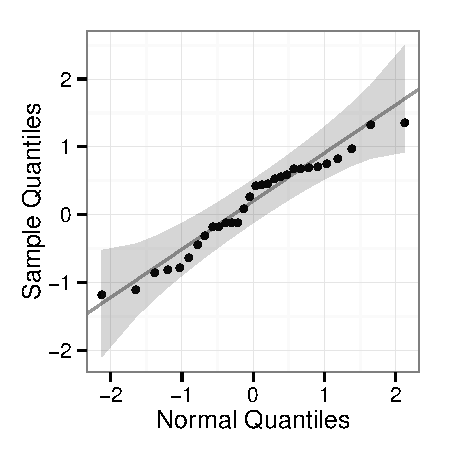
\includegraphics[width=0.35\linewidth]{rotatedQQ-intercept.pdf}
		}
	  \subfloat[Random slope]{
		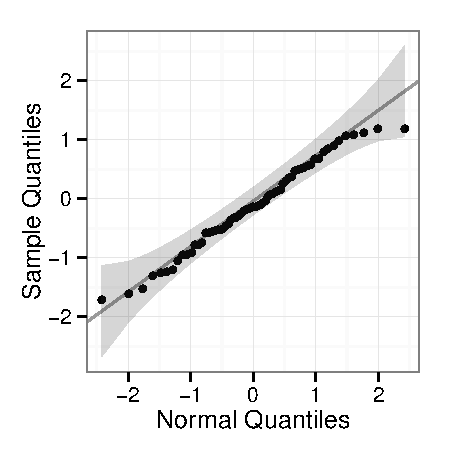
\includegraphics[width=0.35\linewidth]{rotatedQQ-slope.pdf}
		}	
	\caption{\label{fig:rotate-radon} Normal Q-Q plots with pointwise 95\% confidence bands of the marginals rotated random effects. The deviations from normality are much less pronounced than before resulting in the failure to reject the null hypothesis of normality.}
\end{figure}

%\begin{itemize}
%\item Show Q-Q plots for the rotated random effects
%\item Discuss choice of $s$ in this example
%\item Recap root of the problems with the raw random effects (errors not normally distributed; large degree of pooling/shrinkage)
%\end{itemize}

%----------------------------------------------------------------------------------
\section{Discussion}\label{sec:discussion}
%----------------------------------------------------------------------------------

In this paper we have proposed the use of Q-Q plots of rotated residuals as an informal assessment of the distributional assumptions made on the random effects in hierarchical linear model. We have shown that rotated random effects are standardized, uncorrelated, homoscedastic. Following from this result, the pointwise confidence bands shown were not unique to this method, but follow from the development of the normal Q-Q plot (FIND REFERENCE), and were provided as an aid to interpretation, not as a formal test.

Simulation has revealed that tests of normality using the rotated random effects achieve approximately nominal type I error rates with appropriate choice of the length, $s$. This indicates that assessment of the rotated residuals can target the distribution of the random effects in the presence of pooling, which the predicted random effects cannot. The power to detect non-normal random effects distributions is lower than the gold standard, which is to be expected as we have taken linear combinations of predicted random effects in our rotation. The varimax rotation has reduced the impact of the resulting supernormality, but other orthogonal rotations (i.e., quartimax) may perform better and is an area for future investigation. We believe the low power is less troubling than the inflated type I error rates resulting from high levels of confounding, as the detection of a distributional deviation is now trustworthy, which previously not the case for highly confounded models. This indicates that the predicted random effects do contain useful diagnostic information even when models are highly confounded, but not in their ``raw'' state.
 
It is important to note that the procedure outlined in this paper assumes that the covariance structures in the hierarchical linear model are correctly specified. If this is not the case, then we would expect this model violation to affect assessment of the rotated random effect. Therefore, in practice we recommend an assessment of the covariance structures prior to distributional assessment, but it would be of interest to assess the effectiveness of this methodology with robust covariance estimation techniques.

\todo[inline]{I don't quite know how to wrap this all up...}

% If a graphical assessment of the random effects distribution is not desired, then there are other available methods for model assessment \cite[c.f., the $\chi^2$ test proposed by][]{Jiang:2001up}, but they do not lend themselves to graphical inspection. While such goodness-of-fit tests can detect distributional deviations, they do not suggest how the assumption as been violated. 

%The rotated random effects can be used with Q-Q plots, which are familiar to analysts. 
%The use of the rotated random effects results in approximately nominal type I error rates when the dimension, $s$, is properly chosen; however, simulations have revealed that tests using the rotated random effects have low power to detect non-normal alternatives. Despite this fact, the rotated random effects present a method allowing for the predicted random effects to be used in distributional assessment, and when a deviation is detected one has cause to believe this detection, which previously not the case for highly confounded models. Additionally, this method is far less computationally demanding than simulation-based assessments, such as simulation envelopes for Q-Q plots, which are not guaranteed to work in situations with high levels of confounding (see the supplemental materials). Also, orthogonal rotations other than the varimax rotation (such as the quartimax rotation) may provide additional power, and is an area for future investigation. 



%\todo[inline]{
%Summarize everything and talk about future directions (if there are any). I have started a list below}
%\begin{itemize}
%\item Discuss the relative speed of this procedure to a bootstrap procedure
%\item Discuss why we are not using the ``upward'' residuals analysis approach discussed in the lit review chapter.
%\end{itemize}

%----------------------------------------------------------------------------------
\section*{Appendix: Additional technical details}
%----------------------------------------------------------------------------------

We present the proof of the claim that the rotated residuals, $\bm{W}^{*\prime} \widehat{\bm{b}}$, are standardized, uncorrelated, and homoscedastic. Following the developments presented in Section~\ref{sec:rotate} we present this discussion for the random effects assuming that there is only a random intercept. Generalization to the situation with multiple random effects follows as previously discussed.

\begin{proof}
 Let $\bm{A} = \var(\widehat{\bm{b}} | \bm{b})$, $\bm{B} = \var(\widehat{\bm{b}})$, $r = \text{rank}(\bm{B})$, and $\ell = $ the number of elements in $\widehat{\bm{b}}$. Note that by definition $\bm{A}$ and $\bm{B}$ are symmetric and nonnegative definite. Following from above, $\bm{T}_r$ and $\bm{\Lambda}_r$ follow from the spectral (or eigenvalue) decomposition of $\bm{B} = \bm{T_r \Lambda_r T_r}\trans$, and $\bm{U}$ follows from the spectral decomposition of $\bm{A^*} = \bm{\Lambda_r}^{-1/2} \bm{T_r}\trans \bm{A T_r \Lambda_r}^{-1/2} = \bm{U} \bm{\Gamma} \bm{U}\trans$. Then, 
\begin{align*}
\var(\bm{W}^{*\prime} \widehat{\bm{b}}) &= \var(\bm{U}\trans \bm{\Lambda_r}^{-1/2} \bm{T_r}\trans \widehat{\bm{b}})\\
&= (\bm{U}\trans \bm{\Lambda_r}^{-1/2} \bm{T_r}\trans) \var(\widehat{\bm{b}}) (\bm{T_r \Lambda_r}^{-1/2} \bm{U})\\
&= (\bm{U}\trans \bm{\Lambda_r}^{-1/2} \bm{T_r}\trans) \bm{B} (\bm{T_r \Lambda_r}^{-1/2} \bm{U})\\
&= \bm{I}
\end{align*}
proving that the rotated errors are standardized, uncorrelated, and homoscedastic.
\end{proof}
 
%Recall that the trace of a matrix is equal to the sum of its eigenvalues; therefore, minimizing $\tr\left( \bm{B}\ginv\bm{A} \right)$ is equivalent to minimizing the sum of the eigenvalues of $\bm{B}\ginv\bm{A}$. The eigenvalues of $\bm{B}\ginv\bm{A}$ can be found through simultaneous diagonalization
% 
% 
%Write the spectral decomposition of $\bm{B}$ as
%$\bm{B} = \bm{T_r \Lambda_r T_r}\trans$, where $\bm{ \Lambda_r}$ is a diagonal matrix of the nonzero eigenvalues and $\bm{T_r}$ is the matrix of associated eigenvectors.
%Define $\bm{F} = \bm{T_r \Lambda_r}^{1/2}$, which is a full-rank decomposition of $\bm{B}$. The Moore-Penrose inverse of $\bm{F}$ is given by
%\[
%\bm{F}\ginv = (\bm{F}\trans\bm{F})\inv \bm{F}\trans = \bm{\Lambda_r}^{-1/2} \bm{T_r}\trans
%\]
%Now, notice that
%\[
%\bm{F}\ginv \bm{B} (\bm{F}\ginv)\trans = \bm{\Lambda_r}^{-1/2} \bm{T_r}\trans ( \bm{T_r \Lambda_r T_r}\trans ) \bm{T_r \Lambda_r}^{-1/2} =  \bm{I}
%\]
%and define
%\[
%	\bm{A}^* = \bm{F}\ginv \bm{A} (\bm{F}\ginv)\trans
%\]
%Next, we rewrite $\bm{W} = (\bm{F}\ginv)\trans \bm{U}$, where $\bm{U}$ is a nonsingular symmetric matrix. Then \eqref{eq:app1} becomes
%%
%\begin{equation}\label{eq:app2}
%\tr \left[ \left( \bm{U}\trans \bm{F}\ginv \bm{B} (\bm{F}\ginv)\trans \bm{U} \right)\inv 
%\left(\bm{U}\trans \bm{F}\ginv \bm{A} (\bm{F}\ginv)\trans \bm{U} \right) \right]
%=
%\tr \left[ \left( \bm{U}\trans \bm{I} \bm{U} \right)\inv \left( \bm{U}\trans \bm{A}^* \bm{U} \right) \right]
%\end{equation}
%%
%whose derivative with respect to $\bm{U}$ is given by
%%
%\begin{equation}\label{eq:app3}
%-2 \bm{IU} \left( \bm{U}\trans \bm{I} \bm{U} \right)\inv \left( \bm{U}\trans \bm{A}^* \bm{U} \right) \left( \bm{U}\trans \bm{I} \bm{U} \right)\inv + 2 \bm{A}^* \bm{U} \left( \bm{U}\trans \bm{I} \bm{U} \right)\inv
%\end{equation}
%%
%\citep[A.16]{Fukunaga:1990}. Setting \eqref{eq:app3} to zero we find that the solution must satisfy
%%
%\begin{equation}
%\bm{A}^* \bm{U} = \bm{U} \left( \bm{U}\trans \bm{A}^* \bm{U} \right)
%\end{equation}
%%
%
%
%which is of the form of an eigenvalue problem, which is minimized at the eigenvector corresponding to the smallest eigenvalue of  $\bm{A}^*$. Additionally, the value of \eqref{eq:app2} lies between the minimum and maximum eigenvalue of $\bm{A}^*$.
%
%The requirement that $\bm{W}$ be of full rank results in $\bm{W} = \bm{T_r \Lambda_r}^{-1/2} \bm{U}$, where $\bm{U}$ are the eigenvectors of $\bm{A}^*$.
%\end{proof}
%
%More general proofs can be found in \cite{McDonald:1979ca} and \cite{deLeeuw:1982to}.
%
%Next we show that the resulting residuals are standardized, uncorrelated, and homoscedastic.
%
%\begin{proof} Carrying through the notation from above we see that
%\begin{align*}
%\var(\bm{W}^{*\prime} \widehat{\bm{e}}) &= \var(\bm{U}\trans \bm{\Lambda_r}^{-1/2} \bm{T_r}\trans \widehat{\bm{e}})\\
%&= (\bm{U}\trans \bm{\Lambda_r}^{-1/2} \bm{T_r}\trans) \var(\widehat{\bm{e}}) (\bm{T_r \Lambda_r}^{-1/2} \bm{U})\\
%&= (\bm{U}\trans \bm{\Lambda_r}^{-1/2} \bm{T_r}\trans) \bm{B} (\bm{T_r \Lambda_r}^{-1/2} \bm{U})\\
%&= \bm{I}
%\end{align*}
%
%\end{proof}


%----------------------------------------------------------------------------------
%----------------------------------------------------------------------------------
\bibliographystyle{apa}
\bibliography{lcresid_bib}
%----------------------------------------------------------------------------------
%----------------------------------------------------------------------------------

\clearpage

%----------------------------------------------------------------------------------
\appendix
\section{Supplement to ``Are you Normal? The Problem of Confounded Residual Structures in Hierarchical Linear Models''}
%----------------------------------------------------------------------------------

The materials in this document supplement the information presented in ``Are you Normal? The Problem of Confounded Residual Structures in Hierarchical Linear Models''. Section~\ref{supp:evals} presents a simulation study that evaluates the performance of existing proposals for residual analysis for hierarchical linear models. Section~\ref{supp:simstudy} presents the complete results for all simulation settings considered in the paper. 


\subsection{Evaluations of existing proposals}\label{supp:evals}
%--------------------------------------------------

\subsubsection{Model notation}
%--------------------------
Recall that the stacked representation of the hierarchical linear model is given by 
%
\begin{align}\label{eq:hlm}
	\underset{(n \times 1)}{\bm{y}} &= \underset{(n_i \times p)}{\bm{X}} \ \underset{(p \times 1)}{\bm{\beta}} + \underset{(n \times q)}{\bm{Z}_i} \ \underset{(q \times 1)}{\bm{b}} + \underset{(n \times 1)}{\bm{\varepsilon}},\\
	\bm{\varepsilon} & \overset{\text{iid}}{\sim} \mathcal{N}(\bm{0}, \ \bm{R}), \qquad \bm{b} \overset{\text{iid}}{\sim} \mathcal{N}(\bm{0},\ \bm{D}) \nonumber
\end{align}
%
where $\bm{y}$ is a vector of responses, $\bm{X}$ and $\bm{Z}_i$ are design matrices for the fixed and random effects, respectively, $\bm{\beta}$ is a vector of fixed effects, $\bm{b}$ is a vector of random effects, $\bm{\varepsilon}_i$ is a vector of error terms, and $\bm{R}$ and $\bm{D}$ are positive definite covariance matrices. Further, we assume that $\cov(\bm{\varepsilon},\ \bm{b}) = \bm{0}$. The above assumptions imply that, marginally, $\bm{y} \sim \mathcal{N}(\bm{X\beta},\ \bm{V})$ where $\bm{V} = \bm{ZDZ}\trans$.

\subsubsection{Residuals}

In this section we consider residuals that are commonly used to check the distributional assumptions in a hierarchical linear model. For more general discussions of residual analysis for hierarchical linear models we refer the reader to \cite{Haslett:2007vv} and \cite{Nobre:2007ej}.

\paragraph{Marginal residuals.} 
%-----------------------------
The marginal distribution of $\bm{y}$ leads to the marginal residuals which are defined as
%
\begin{equation}\label{eq:marginalresid}
\widehat{\bm{\zeta}}  = \bm{y} - \bm{X} \widehat{\bm{\beta}} =  \bm{V P y}
\end{equation}
%
where $ \bm{P} = \bm{V\inv} - \bm{V\inv X} \left( \bm{X\trans V\inv X} \right) \bm{X \trans V\inv}$, which reveal how the observations deviate from the global trend. The use of these residuals for distributional assessment provides an omnibus assessment of goodness-of-fit as the marginal residuals are a linear combination of the other residual quantities; however, this assessment requires the empirical distribution of the marginal residuals to resemble true distribution. Asymptotically, the variance of the marginal residuals is $\var(\widehat{\zeta}) = \bm{V}$ leading to correlated residuals. To obtain asymptotically uncorrelated residuals the marginal residuals can be scaled by the Cholesky root of $\bm{V}$ \citep{Houseman:2004gq}, $\bm{C}$, yielding
%
\begin{equation}\label{eq:choleskyresid}
\bm{z}_{\zeta}  = \bm{C}\inv \widehat{\bm{\zeta}}
\end{equation}
%


\paragraph{Level-1 residuals.}
%-----------------------------
The distribution of $\bm{y}$ conditional on the random effects, $\bm{b}$, is given by
%
\begin{equation}\label{eq:marginalmodel}
	\bm{y} | \bm{b} \sim \mathcal{N}( \bm{X\beta} + \bm{Zb},\ \bm{R} ),
\end{equation}
%
and leads to the level-1 residuals, commonly referred to as the error terms, which are defined as
%
\begin{equation}\label{eq:lev1resid}
	\widehat{\bm{\varepsilon}} = \bm{y} - \bm{X \widehat{\beta}} + \bm{Z \widehat{b}} = \bm{R P y}
\end{equation}
%
and reveal the deviations of the observations from the conditional model. The variance of the level-1 residuals is given by $\var(\widehat{\bm{\varepsilon}}) = \bm{ R P R }$, so studentized level-1 residuals can be obtained by 
%
\begin{equation}\label{eq:lev1-std}
\bm{z}_{\varepsilon} =  \text{diag} \left(\bm{RPR} \right)^{-1/2} \widehat{\bm{\varepsilon}}
\end{equation}
%
which have been recommended for distributional assessment \citep{Nobre:2007ej}. An alternative approach is recommended by \cite[Section 4.3]{Pinhiero:2000vf}, who suggest use of the Pearson residuals obtained, which are obtained by dividing the predicted residuals by the estimated within-group standard deviation, $\widehat{\sigma}_\varepsilon$. 



\paragraph{Level-2 residuals.}
%-----------------------------
The final type of residual we consider is the the best linear unbiased predictor (BLUP) of the random effects, providing insight into the differences between the marginal (global) and conditional models. By definition, the BLUP of $\bm{b}$ is
%
\begin{equation}\label{eq:lev2resid}
\widehat{\bm{b}} = \bm{D Z\trans V\inv} \left( \bm{y} - \bm{X \widehat{\beta}} \right) = \bm{D Z\trans P y}
\end{equation}
%
which has $\var(\widehat{\bm{b}}) = \bm{DZ\trans P ZD}$. 
%Rewriting $\var(\widehat{\bm{b}})$ as
%%
%\begin{equation}
%\bm{DZ\trans P ZD} = \bm{DZ\trans} \bm{V\inv} \left( \bm{V} - \bm{ X} \left( \bm{X\trans V\inv X} \right) \bm{X \trans} \right) \bm{V\inv} \bm{ZD}
%\end{equation}
%%
%leads to two 
For distributional assessment of the BLUPs it makes sense to examine each random effect individually, though \cite{Lange:1989uu} suggest the examination of linear combinations of standardized BLUPs. Rewritting the definition of $\var(\widehat{\bm{b}})$
%
\begin{equation}
\bm{DZ\trans P ZD} = \bm{DZ\trans} \bm{V\inv} \left( \bm{V} - \bm{ X} \left( \bm{X\trans V\inv X} \right) \bm{X \trans} \right) \bm{V\inv} \bm{ZD}
\end{equation}
%
leads to two similar standardizations of the BLUPs. The first utilizes the fact that when the number of groups is large $\bm{ X} \left( \bm{X\trans V\inv X} \right)$ will be small \citep{Goldstein:2003}, so for a large number of groups standardized BLUPs can be calculated by
%
\begin{equation}\label{eq:lev2-std1}
\bm{z}_{b} = \text{diag} \left(\bm{DZ\trans V\inv ZD}\right)^{-1/2} \widehat{\bm{b}}
\end{equation}
%
This formulation is the same used by \cite{Lange:1989uu} (discussed below).
%, who suggest creating weighted Q-Q plots \citep{Dempster:1985tr} to assess the distributional assumptions. Note that standardized linear combinations of the BLUPs follow in the usual way. 
The second standardization applies for all sample sizes and is given by
%
\begin{equation}\label{eq:lev2-std2}
\bm{z}_{b} = \text{diag} \left(\bm{DZ\trans P ZD}\right)^{-1/2} \widehat{\bm{b}}
\end{equation}
%


\paragraph{Weighted Q-Q plots}
%------------------------------

As an alternative to Q-Q plots constructed from the BLUPs \cite{Lange:1989uu} propose using weighted Q-Q plots of standardized linear combinations of the BLUPs, $\bm{C\trans}\widehat{\bm{b}}$,
%
\begin{equation}
z_{b} = \text{diag} \left(\bm{C\trans DZ\trans V\inv ZDC}\right)^{-1/2} \bm{C\trans}\widehat{\bm{b}}
\end{equation}
%
The specific form of $\bm{C}$ chosen highlight different departures from distributional assumptions---for example, $\bm{C}$s can be chosen to extract the random slope and the random intercept terms individually. When the random effects may be correlated, \citeauthor{Lange:1989uu} suggest examining a range of additional linear combinations in-between the two marginal random effects either through manual specification of $\bm{C}$ or projection pursuit.
After choosing $\bm{C}$ a weighted Q-Q plot is constructed by comparing the weighted empirical cumulative distribution function
%
\begin{equation}
F_m^*(x) = \sum_{i=1}^{m} I(x - z_{b_i} \geq 0) w_i \bigg/ \sum_{i=1}^{m} w_i, 
\end{equation}
%
where $w_i$ is the $i$th element of $\bm{C\trans DZ\trans V\inv ZDC}$, to $\Phi\inv \left ( F_m^*(z_{b_i}) \right)$. For balanced group sizes this simplifies to the unweighted Q-Q plot of $\bm{z}_b$.
%

\paragraph{Simulation-based approaches}
%---------------------------------------

All of the above approaches to checking the distributional assumptions rely on the use of interrelated residuals, which has been reported to be problematic \citep{HildenMinton:1995wh, Verbeke:1996va}.  
One alternative that has been proposed to overcome this problem is the use of the parametric bootstrap to develop point-wise and simultaneous confidence bands for Q-Q plots. We evaluate the potential of this method using bootstrap tests of normality.


\subsubsection{Simulation study}\label{supp:simstudy}
%--------------------------------------------------

To evaluate the above proposals we carried out a simulation study under the same settings as in the paper, with the only difference being that the original $\bm{Z}$ was used for data generation. To evaluate the bootstrap tests of normality, a null distribution of 5000 simulated test statistics for each situation was used.

Tables~\ref{tab:eval1}--\ref{tab:evalmarginal} present the results of using standard normality tests to assess the distributional assumptions of the residuals from a hierarchical model. The gray background on the table indicates which simulation settings approximately align with type I error, the other rows present estimated power. Tables~\ref{tab:boot1}--\ref{tab:bootmarginal} present the results of the bootstrap tests for normality. Table~\ref{tab:langeryan} presents the results of using a weighted CDF to evaluate the normality of the random effects, in this case the null distribution was obtained using the parametric bootstrap.

Based on the simulation results it is clear that none of the residual-based diagnostics for assessing distributional assumptions are appropriate in all situations. The error terms can be targeted by the use of either by the use of studentized residuals or a parametric bootstrap; however, the assessment of this assumption is less critical. The random effects, on which predictive inference relies, cannot be targeted by the current methods when the residual variance is larger than the variance component associated with the random effects, a situation that is often encountered in practice. Additionally, use of the parametric bootstrap---to construct simulation envelopes for Q-Q plots, for example---does not appear to remedy this situation based on the performance of the bootstrap tests. Finally, we have shown \citeauthor{Lange:1989uu}'s weighted Q-Q plots also cannot target the random effects distribution when the residual variance is large, resulting in inflated type I error rates for both random effects, and the error terms overly influencing tests for the random slope.


%&&&&&&&&&&&&&&&&&&&&&&&&&&&&&&&&&&&&&&&&&&&&&&&&&&&&&&&&&&&&&&&&&&&&&&&&&&&&&&
% Correct model
%&&&&&&&&&&&&&&&&&&&&&&&&&&&&&&&&&&&&&&&&&&&&&&&&&&&&&&&&&&&&&&&&&&&&&&&&&&&&&&


%------------------------------------------------
% Naive tests
%------------------------------------------------

%%% Level-1 residuals
\begin{table}[ht]
\centering
\caption{\label{tab:eval1} Proportion of tests rejecting the null hypothesis of normality of the error terms.}
\begin{scriptsize}
\begin{tabular}{ll p{.1cm} c p{.1cm} rrr p{.1cm} rrr p{.1cm} rrr}
  \hline
  \multicolumn{2}{c}{Distributions}& & Nominal & &  \multicolumn{3}{c}{Raw residuals} & & \multicolumn{3}{c}{Pearson residuals} & & \multicolumn{3}{c}{Studentized residuals}\\ \cline{1-2} \cline{6-8} \cline{10-12} \cline{14-16}
  Errors & Random effects & & $\alpha$ & & AD & CVM & KS & & AD & CVM & KS & & AD & CVM & KS \\ 
   \hline
& && && \multicolumn{9}{c}{$\sigma_{\varepsilon}^2 = 4$, \ \ $\sigma_{b_0}^2 = \sigma_{b_1}^2 = 1$} \\ \cline{6-16}

\rowcolor{gray!20} Normal       & Normal       && 0.05 && 0.07 & 0.06 & 0.06 && 0.07 & 0.06 & 0.06 && 0.04 & 0.04 & 0.04 \\ 
\rowcolor{gray!20}             &              && 0.10 && 0.13 & 0.12 & 0.12 && 0.13 & 0.12 & 0.12 && 0.09 & 0.09 & 0.10 \\ 
\rowcolor{gray!20}             & Heavy tailed && 0.05 && 0.07 & 0.08 & 0.06 && 0.07 & 0.08 & 0.06 && 0.05 & 0.05 & 0.05 \\ 
\rowcolor{gray!20}             &              && 0.10 && 0.14 & 0.13 & 0.14 && 0.14 & 0.13 & 0.14 && 0.11 & 0.11 & 0.10 \\ 
\rowcolor{gray!20}             & Skewed       && 0.05 && 0.07 & 0.06 & 0.06 && 0.07 & 0.06 & 0.06 && 0.04 & 0.04 & 0.05 \\ 
\rowcolor{gray!20}             &              && 0.10 && 0.13 & 0.12 & 0.13 && 0.13 & 0.12 & 0.13 && 0.09 & 0.09 & 0.10 \\ 
             &&&&&&&&&&&&&&&\\
Heavy tailed & Normal       && 0.05 && 1.00 & 1.00 & 1.00 && 1.00 & 1.00 & 1.00 && 1.00 & 1.00 & 1.00 \\ 
             &              && 0.10 && 1.00 & 1.00 & 1.00 && 1.00 & 1.00 & 1.00 && 1.00 & 1.00 & 1.00 \\ 
             & Heavy tailed && 0.05 && 1.00 & 1.00 & 1.00 && 1.00 & 1.00 & 1.00 && 1.00 & 1.00 & 1.00 \\ 
             &              && 0.10 && 1.00 & 1.00 & 1.00 && 1.00 & 1.00 & 1.00 && 1.00 & 1.00 & 1.00 \\ 
             & Skewed       && 0.05 && 1.00 & 1.00 & 1.00 && 1.00 & 1.00 & 1.00 && 1.00 & 1.00 & 1.00 \\ 
             &              && 0.10 && 1.00 & 1.00 & 1.00 && 1.00 & 1.00 & 1.00 && 1.00 & 1.00 & 1.00 \\ 
             &&&&&&&&&&&&&&&\\
Skewed       & Normal       && 0.05 && 1.00 & 1.00 & 1.00 && 1.00 & 1.00 & 1.00 && 1.00 & 1.00 & 1.00 \\ 
             &              && 0.10 && 1.00 & 1.00 & 1.00 && 1.00 & 1.00 & 1.00 && 1.00 & 1.00 & 1.00 \\ 
             & Heavy tailed && 0.05 && 1.00 & 1.00 & 1.00 && 1.00 & 1.00 & 1.00 && 1.00 & 1.00 & 1.00 \\ 
             &              && 0.10 && 1.00 & 1.00 & 1.00 && 1.00 & 1.00 & 1.00 && 1.00 & 1.00 & 1.00 \\ 
             & Skewed       && 0.05 && 1.00 & 1.00 & 1.00 && 1.00 & 1.00 & 1.00 && 1.00 & 1.00 & 1.00 \\ 
             &              && 0.10 && 1.00 & 1.00 & 1.00 && 1.00 & 1.00 & 1.00 && 1.00 & 1.00 & 1.00 \\ 

&&&&&&&&&&&&&&&\\
& && && \multicolumn{9}{c}{$\sigma_{\varepsilon}^2 = 1$, \ \ $\sigma_{b_0}^2 = \sigma_{b_1}^2 = 1$} \\ \cline{6-16}

\rowcolor{gray!20} Normal       & Normal       && 0.05 &&  0.05 & 0.05 & 0.04 && 0.05 & 0.05 & 0.04 && 0.04 & 0.04 & 0.04 \\ 
\rowcolor{gray!20}              &              && 0.10 &&  0.11 & 0.10 & 0.09 && 0.11 & 0.10 & 0.09 && 0.09 & 0.09 & 0.08 \\ 
\rowcolor{gray!20}              & Heavy tailed && 0.05 &&  0.07 & 0.06 & 0.06 && 0.07 & 0.06 & 0.06 && 0.05 & 0.06 & 0.05 \\ 
\rowcolor{gray!20}              &              && 0.10 &&  0.13 & 0.12 & 0.11 && 0.13 & 0.12 & 0.11 && 0.11 & 0.11 & 0.10 \\ 
\rowcolor{gray!20}              & Skewed       && 0.05 &&  0.05 & 0.05 & 0.05 && 0.05 & 0.05 & 0.05 && 0.04 & 0.04 & 0.04 \\ 
\rowcolor{gray!20}              &              && 0.10 &&  0.10 & 0.09 & 0.11 && 0.10 & 0.09 & 0.11 && 0.08 & 0.09 & 0.10 \\ 
              &&&&&&&&&&&&&&&\\
 Heavy tailed & Normal       && 0.05 &&  1.00 & 1.00 & 1.00 && 1.00 & 1.00 & 1.00 && 1.00 & 1.00 & 1.00 \\ 
              &              && 0.10 &&  1.00 & 1.00 & 1.00 && 1.00 & 1.00 & 1.00 && 1.00 & 1.00 & 1.00 \\ 
              & Heavy tailed && 0.05 &&  1.00 & 1.00 & 1.00 && 1.00 & 1.00 & 1.00 && 1.00 & 1.00 & 1.00 \\ 
              &              && 0.10 &&  1.00 & 1.00 & 1.00 && 1.00 & 1.00 & 1.00 && 1.00 & 1.00 & 1.00 \\ 
              & Skewed       && 0.05 &&  1.00 & 1.00 & 1.00 && 1.00 & 1.00 & 1.00 && 1.00 & 1.00 & 1.00 \\ 
              &              && 0.10 &&  1.00 & 1.00 & 1.00 && 1.00 & 1.00 & 1.00 && 1.00 & 1.00 & 1.00 \\ 
              &&&&&&&&&&&&&&&\\
 Skewed       & Normal       && 0.05 &&  1.00 & 1.00 & 1.00 && 1.00 & 1.00 & 1.00 && 1.00 & 1.00 & 1.00 \\ 
              &              && 0.10 &&  1.00 & 1.00 & 1.00 && 1.00 & 1.00 & 1.00 && 1.00 & 1.00 & 1.00 \\ 
              & Heavy tailed && 0.05 &&  1.00 & 1.00 & 1.00 && 1.00 & 1.00 & 1.00 && 1.00 & 1.00 & 1.00 \\ 
              &              && 0.10 &&  1.00 & 1.00 & 1.00 && 1.00 & 1.00 & 1.00 && 1.00 & 1.00 & 1.00 \\ 
              & Skewed       && 0.05 &&  1.00 & 1.00 & 1.00 && 1.00 & 1.00 & 1.00 && 1.00 & 1.00 & 1.00 \\ 
              &              && 0.10 &&  1.00 & 1.00 & 1.00 && 1.00 & 1.00 & 1.00 && 1.00 & 1.00 & 1.00 \\ 

&&&&&&&&&&&&&&&\\
& && && \multicolumn{9}{c}{$\sigma_{\varepsilon}^2 = 1$, \ \ $\sigma_{b_0}^2 = \sigma_{b_1}^2 = 4$} \\ \cline{6-16}

\rowcolor{gray!20} Normal       & Normal       && 0.05 &&  0.10 & 0.09 & 0.07 && 0.10 & 0.09 & 0.07 && 0.05 & 0.04 & 0.04 \\ 
\rowcolor{gray!20}             &              && 0.10 &&  0.17 & 0.17 & 0.15 && 0.17 & 0.17 & 0.15 && 0.09 & 0.09 & 0.09 \\ 
\rowcolor{gray!20}             & Heavy tailed && 0.05 &&  0.11 & 0.11 & 0.10 && 0.11 & 0.11 & 0.10 && 0.06 & 0.06 & 0.05 \\ 
\rowcolor{gray!20}             &              && 0.10 &&  0.19 & 0.19 & 0.19 && 0.19 & 0.19 & 0.19 && 0.12 & 0.11 & 0.12 \\ 
\rowcolor{gray!20}             & Skewed       && 0.05 &&  0.10 & 0.10 & 0.09 && 0.10 & 0.10 & 0.09 && 0.05 & 0.05 & 0.06 \\ 
\rowcolor{gray!20}             &              && 0.10 &&  0.18 & 0.18 & 0.17 && 0.18 & 0.18 & 0.17 && 0.11 & 0.11 & 0.11 \\ 
             &&&&&&&&&&&&&&&\\
Heavy tailed & Normal       && 0.05 &&  1.00 & 1.00 & 1.00 && 1.00 & 1.00 & 1.00 && 1.00 & 1.00 & 1.00 \\ 
             &              && 0.10 &&  1.00 & 1.00 & 1.00 && 1.00 & 1.00 & 1.00 && 1.00 & 1.00 & 1.00 \\ 
             & Heavy tailed && 0.05 &&  1.00 & 1.00 & 1.00 && 1.00 & 1.00 & 1.00 && 1.00 & 1.00 & 1.00 \\ 
             &              && 0.10 &&  1.00 & 1.00 & 1.00 && 1.00 & 1.00 & 1.00 && 1.00 & 1.00 & 1.00 \\ 
             & Skewed       && 0.05 &&  1.00 & 1.00 & 1.00 && 1.00 & 1.00 & 1.00 && 1.00 & 1.00 & 1.00 \\ 
             &              && 0.10 &&  1.00 & 1.00 & 1.00 && 1.00 & 1.00 & 1.00 && 1.00 & 1.00 & 1.00 \\ 
             &&&&&&&&&&&&&&&\\
Skewed       & Normal       && 0.05 &&  1.00 & 1.00 & 1.00 && 1.00 & 1.00 & 1.00 && 1.00 & 1.00 & 1.00 \\ 
             &              && 0.10 &&  1.00 & 1.00 & 1.00 && 1.00 & 1.00 & 1.00 && 1.00 & 1.00 & 1.00 \\ 
             & Heavy tailed && 0.05 &&  1.00 & 1.00 & 1.00 && 1.00 & 1.00 & 1.00 && 1.00 & 1.00 & 1.00 \\ 
             &              && 0.10 &&  1.00 & 1.00 & 1.00 && 1.00 & 1.00 & 1.00 && 1.00 & 1.00 & 1.00 \\ 
             & Skewed       && 0.05 &&  1.00 & 1.00 & 1.00 && 1.00 & 1.00 & 1.00 && 1.00 & 1.00 & 1.00 \\ 
             &              && 0.10 &&  1.00 & 1.00 & 1.00 && 1.00 & 1.00 & 1.00 && 1.00 & 1.00 & 1.00 \\ 


   \hline
\end{tabular}
\end{scriptsize}
\end{table}

%%% Level-2 residuals
\begin{table}[ht]
\centering
\caption{\label{tab:evalb0} Proportion of tests rejecting the null hypothesis of normality of the random intercept.}
\begin{scriptsize}
\begin{tabular}{ll p{.1cm} c p{.1cm} rrr p{.1cm} rrr p{.1cm} rrr}
  \hline
  \multicolumn{2}{c}{Distributions}& & Nominal & &  \multicolumn{3}{c}{Raw residuals} & & \multicolumn{3}{c}{Pearson residuals} & & \multicolumn{3}{c}{Studentized residuals}\\ \cline{1-2} \cline{6-8} \cline{10-12} \cline{14-16}
  Random effects & Errors & & $\alpha$ & & AD & CVM & KS & & AD & CVM & KS & & AD & CVM & KS \\ 
   \hline
& && && \multicolumn{9}{c}{$\sigma_{\varepsilon}^2 = 4$, \ \ $\sigma_{b_0}^2 = \sigma_{b_1}^2 = 1$} \\ \cline{6-16}

\rowcolor{gray!20} Normal       & Normal       && 0.05 &&   0.05 & 0.05 & 0.05 && 0.05 & 0.05 & 0.06 && 0.05 & 0.05 & 0.06 \\ 
\rowcolor{gray!20}             &              && 0.10 &&   0.10 & 0.10 & 0.10 && 0.11 & 0.10 & 0.12 && 0.11 & 0.10 & 0.12 \\ 
\rowcolor{gray!20}             & Heavy tailed && 0.05 &&   0.15 & 0.13 & 0.12 && 0.17 & 0.15 & 0.13 && 0.17 & 0.15 & 0.13 \\ 
\rowcolor{gray!20}             &              && 0.10 &&   0.22 & 0.20 & 0.20 && 0.26 & 0.23 & 0.21 && 0.26 & 0.23 & 0.20 \\ 
\rowcolor{gray!20}             & Skewed       && 0.05 &&   0.16 & 0.15 & 0.13 && 0.18 & 0.17 & 0.14 && 0.18 & 0.17 & 0.14 \\ 
\rowcolor{gray!20}             &              && 0.10 &&   0.25 & 0.23 & 0.21 && 0.28 & 0.25 & 0.22 && 0.28 & 0.25 & 0.21 \\ 
             &&&&&&&&&&&&&&&\\
Heavy tailed & Normal       && 0.05 &&   0.27 & 0.24 & 0.19 && 0.28 & 0.26 & 0.21 && 0.28 & 0.26 & 0.21 \\ 
             &              && 0.10 &&   0.35 & 0.31 & 0.28 && 0.36 & 0.34 & 0.30 && 0.36 & 0.33 & 0.30 \\ 
             & Heavy tailed && 0.05 &&   0.49 & 0.45 & 0.35 && 0.51 & 0.46 & 0.36 && 0.50 & 0.46 & 0.36 \\ 
             &              && 0.10 &&   0.58 & 0.54 & 0.46 && 0.60 & 0.55 & 0.47 && 0.60 & 0.55 & 0.47 \\ 
             & Skewed       && 0.05 &&   0.52 & 0.48 & 0.36 && 0.55 & 0.50 & 0.40 && 0.55 & 0.50 & 0.40 \\ 
             &              && 0.10 &&   0.62 & 0.59 & 0.51 && 0.65 & 0.60 & 0.53 && 0.65 & 0.60 & 0.52 \\
             &&&&&&&&&&&&&&&\\ 
Skewed       & Normal       && 0.05 &&   0.51 & 0.48 & 0.39 && 0.51 & 0.49 & 0.38 && 0.51 & 0.49 & 0.39 \\ 
             &              && 0.10 &&   0.61 & 0.58 & 0.51 && 0.61 & 0.59 & 0.52 && 0.60 & 0.58 & 0.52 \\ 
             & Heavy tailed && 0.05 &&   0.73 & 0.69 & 0.58 && 0.73 & 0.70 & 0.59 && 0.73 & 0.70 & 0.59 \\ 
             &              && 0.10 &&   0.80 & 0.77 & 0.69 && 0.81 & 0.78 & 0.70 && 0.80 & 0.78 & 0.70 \\ 
             & Skewed       && 0.05 &&   0.87 & 0.83 & 0.70 && 0.87 & 0.82 & 0.69 && 0.86 & 0.83 & 0.69 \\ 
             &              && 0.10 &&   0.92 & 0.89 & 0.80 && 0.91 & 0.88 & 0.80 && 0.91 & 0.88 & 0.80 \\ 

&&&&&&&&&&&&&&&\\
& && && \multicolumn{9}{c}{$\sigma_{\varepsilon}^2 = 1$, \ \ $\sigma_{b_0}^2 = \sigma_{b_1}^2 = 1$} \\ \cline{6-16}
\rowcolor{gray!20} Normal       & Normal       && 0.05 &&   0.05 & 0.05 & 0.04 && 0.05 & 0.05 & 0.04 && 0.05 & 0.05 & 0.04 \\ 
\rowcolor{gray!20}             &              && 0.10 &&   0.09 & 0.09 & 0.08 && 0.09 & 0.08 & 0.08 && 0.08 & 0.08 & 0.08 \\ 
\rowcolor{gray!20}             & Heavy tailed && 0.05 &&   0.07 & 0.07 & 0.06 && 0.07 & 0.07 & 0.06 && 0.07 & 0.07 & 0.06 \\ 
\rowcolor{gray!20}             &              && 0.10 &&   0.12 & 0.12 & 0.11 && 0.12 & 0.11 & 0.11 && 0.12 & 0.11 & 0.11 \\ 
\rowcolor{gray!20}             & Skewed       && 0.05 &&   0.06 & 0.06 & 0.07 && 0.06 & 0.06 & 0.06 && 0.06 & 0.06 & 0.06 \\ 
\rowcolor{gray!20}             &              && 0.10 &&   0.11 & 0.11 & 0.12 && 0.12 & 0.12 & 0.12 && 0.12 & 0.11 & 0.12 \\
             &&&&&&&&&&&&&&&\\  
Heavy tailed & Normal       && 0.05 &&   0.55 & 0.50 & 0.42 && 0.52 & 0.48 & 0.40 && 0.52 & 0.48 & 0.40 \\ 
             &              && 0.10 &&   0.63 & 0.60 & 0.51 && 0.60 & 0.56 & 0.51 && 0.60 & 0.56 & 0.52 \\ 
             & Heavy tailed && 0.05 &&   0.63 & 0.58 & 0.49 && 0.60 & 0.56 & 0.47 && 0.60 & 0.56 & 0.47 \\ 
             &              && 0.10 &&   0.71 & 0.68 & 0.60 && 0.68 & 0.63 & 0.56 && 0.68 & 0.63 & 0.56 \\ 
             & Skewed       && 0.05 &&   0.62 & 0.57 & 0.47 && 0.61 & 0.55 & 0.46 && 0.61 & 0.55 & 0.46 \\ 
             &              && 0.10 &&   0.71 & 0.66 & 0.58 && 0.69 & 0.65 & 0.57 && 0.69 & 0.64 & 0.57 \\ 
             &&&&&&&&&&&&&&&\\ 
Skewed       & Normal       && 0.05 &&   0.93 & 0.92 & 0.86 && 0.93 & 0.91 & 0.86 && 0.93 & 0.91 & 0.85 \\ 
             &              && 0.10 &&   0.96 & 0.94 & 0.91 && 0.96 & 0.94 & 0.90 && 0.95 & 0.94 & 0.90 \\ 
             & Heavy tailed && 0.05 &&   0.97 & 0.96 & 0.89 && 0.97 & 0.96 & 0.88 && 0.97 & 0.96 & 0.88 \\ 
             &              && 0.10 &&   0.99 & 0.98 & 0.94 && 0.99 & 0.98 & 0.94 && 0.99 & 0.98 & 0.94 \\ 
             & Skewed       && 0.05 &&   0.98 & 0.96 & 0.90 && 0.98 & 0.97 & 0.90 && 0.98 & 0.97 & 0.91 \\ 
             &              && 0.10 &&   0.99 & 0.97 & 0.95 && 0.99 & 0.98 & 0.94 && 0.99 & 0.98 & 0.95 \\ 


&&&&&&&&&&&&&&&\\
& && && \multicolumn{9}{c}{$\sigma_{\varepsilon}^2 = 1$, \ \ $\sigma_{b_0}^2 = \sigma_{b_1}^2 = 4$} \\ \cline{6-16}

\rowcolor{gray!20} Normal       & Normal       && 0.05 &&  0.05 & 0.05 & 0.05 && 0.05 & 0.05 & 0.04 && 0.05 & 0.05 & 0.04 \\ 
\rowcolor{gray!20}             &              && 0.10 &&  0.10 & 0.09 & 0.09 && 0.10 & 0.09 & 0.09 && 0.10 & 0.09 & 0.09 \\ 
\rowcolor{gray!20}             & Heavy tailed && 0.05 &&  0.04 & 0.04 & 0.05 && 0.05 & 0.05 & 0.05 && 0.05 & 0.05 & 0.05 \\ 
\rowcolor{gray!20}             &              && 0.10 &&  0.09 & 0.09 & 0.09 && 0.09 & 0.09 & 0.09 && 0.09 & 0.09 & 0.09 \\ 
\rowcolor{gray!20}             & Skewed       && 0.05 &&  0.04 & 0.04 & 0.03 && 0.04 & 0.04 & 0.03 && 0.04 & 0.04 & 0.03 \\ 
\rowcolor{gray!20}             &              && 0.10 &&  0.09 & 0.09 & 0.08 && 0.10 & 0.09 & 0.08 && 0.09 & 0.09 & 0.08 \\ 
             &&&&&&&&&&&&&&&\\
Heavy tailed & Normal       && 0.05 &&  0.68 & 0.63 & 0.54 && 0.68 & 0.63 & 0.54 && 0.68 & 0.63 & 0.54 \\ 
             &              && 0.10 &&  0.75 & 0.71 & 0.63 && 0.75 & 0.70 & 0.64 && 0.75 & 0.71 & 0.64 \\ 
             & Heavy tailed && 0.05 &&  0.71 & 0.67 & 0.57 && 0.71 & 0.67 & 0.58 && 0.71 & 0.67 & 0.57 \\ 
             &              && 0.10 &&  0.78 & 0.76 & 0.68 && 0.79 & 0.76 & 0.67 && 0.79 & 0.75 & 0.67 \\ 
             & Skewed       && 0.05 &&  0.70 & 0.68 & 0.57 && 0.70 & 0.67 & 0.56 && 0.70 & 0.67 & 0.56 \\ 
             &              && 0.10 &&  0.78 & 0.74 & 0.68 && 0.78 & 0.74 & 0.68 && 0.78 & 0.74 & 0.67 \\ 
             &&&&&&&&&&&&&&&\\
Skewed       & Normal       && 0.05 &&  1.00 & 0.99 & 0.97 && 1.00 & 0.99 & 0.97 && 1.00 & 0.99 & 0.97 \\ 
             &              && 0.10 &&  1.00 & 1.00 & 0.99 && 1.00 & 1.00 & 0.99 && 1.00 & 1.00 & 0.99 \\ 
             & Heavy tailed && 0.05 &&  1.00 & 1.00 & 0.98 && 1.00 & 1.00 & 0.98 && 1.00 & 1.00 & 0.98 \\ 
             &              && 0.10 &&  1.00 & 1.00 & 0.99 && 1.00 & 1.00 & 0.99 && 1.00 & 1.00 & 0.99 \\ 
             & Skewed       && 0.05 &&  1.00 & 1.00 & 0.98 && 1.00 & 1.00 & 0.98 && 1.00 & 1.00 & 0.98 \\ 
             &              && 0.10 &&  1.00 & 1.00 & 0.99 && 1.00 & 1.00 & 0.99 && 1.00 & 1.00 & 0.99 \\ 


   \hline
\end{tabular}
\end{scriptsize}
\end{table}


\begin{table}[ht]
\centering
\caption{\label{tab:evalb1} Proportion of tests rejecting the null hypothesis of normality of the random slope.}
\begin{scriptsize}
\begin{tabular}{ll p{.1cm} c p{.1cm} rrr p{.1cm} rrr p{.1cm} rrr}
  \hline
  \multicolumn{2}{c}{Distributions}& & Nominal & &  \multicolumn{3}{c}{Raw residuals} & & \multicolumn{3}{c}{Pearson residuals} & & \multicolumn{3}{c}{Studentized residuals}\\ \cline{1-2} \cline{6-8} \cline{10-12} \cline{14-16}
  Random effects & Errors & & $\alpha$ & & AD & CVM & KS & & AD & CVM & KS & & AD & CVM & KS \\ 
   \hline
& && && \multicolumn{9}{c}{$\sigma_{\varepsilon}^2 = 4$, \ \ $\sigma_{b_0}^2 = \sigma_{b_1}^2 = 1$} \\ \cline{6-16}

\rowcolor{gray!20} Normal       & Normal       && 0.05 &&   1.00 & 1.00 & 1.00 && 0.05 & 0.05 & 0.06 && 0.05 & 0.05 & 0.06 \\ 
\rowcolor{gray!20}             &              && 0.10 &&   1.00 & 1.00 & 1.00 && 0.10 & 0.10 & 0.10 && 0.10 & 0.10 & 0.10 \\ 
\rowcolor{gray!20}             & Heavy tailed && 0.05 &&   1.00 & 1.00 & 1.00 && 0.26 & 0.24 & 0.19 && 0.26 & 0.24 & 0.19 \\ 
\rowcolor{gray!20}             &              && 0.10 &&   1.00 & 1.00 & 1.00 && 0.35 & 0.32 & 0.27 && 0.35 & 0.32 & 0.27 \\ 
\rowcolor{gray!20}             & Skewed       && 0.05 &&   1.00 & 1.00 & 1.00 && 0.33 & 0.31 & 0.24 && 0.33 & 0.31 & 0.24 \\ 
\rowcolor{gray!20}             &              && 0.10 &&   1.00 & 1.00 & 1.00 && 0.41 & 0.38 & 0.34 && 0.41 & 0.38 & 0.34 \\ 
             &&&&&&&&&&&&&&&\\
Heavy tailed & Normal       && 0.05 &&   1.00 & 1.00 & 1.00 && 0.13 & 0.12 & 0.09 && 0.13 & 0.12 & 0.09 \\ 
             &              && 0.10 &&   1.00 & 1.00 & 1.00 && 0.18 & 0.19 & 0.17 && 0.18 & 0.19 & 0.17 \\ 
             & Heavy tailed && 0.05 &&   1.00 & 1.00 & 1.00 && 0.40 & 0.36 & 0.29 && 0.40 & 0.36 & 0.29 \\ 
             &              && 0.10 &&   1.00 & 1.00 & 1.00 && 0.49 & 0.44 & 0.37 && 0.49 & 0.45 & 0.37 \\ 
             & Skewed       && 0.05 &&   1.00 & 1.00 & 1.00 && 0.49 & 0.46 & 0.37 && 0.49 & 0.46 & 0.37 \\ 
             &              && 0.10 &&   1.00 & 1.00 & 1.00 && 0.59 & 0.56 & 0.50 && 0.59 & 0.56 & 0.49 \\
             &&&&&&&&&&&&&&&\\ 
Skewed       & Normal       && 0.05 &&   1.00 & 1.00 & 1.00 && 0.12 & 0.11 & 0.10 && 0.12 & 0.11 & 0.10 \\ 
             &              && 0.10 &&   1.00 & 1.00 & 1.00 && 0.17 & 0.16 & 0.16 && 0.18 & 0.16 & 0.16 \\ 
             & Heavy tailed && 0.05 &&   1.00 & 1.00 & 1.00 && 0.41 & 0.37 & 0.30 && 0.40 & 0.37 & 0.30 \\ 
             &              && 0.10 &&   1.00 & 1.00 & 1.00 && 0.51 & 0.47 & 0.39 && 0.51 & 0.47 & 0.39 \\ 
             & Skewed       && 0.05 &&   1.00 & 1.00 & 1.00 && 0.59 & 0.56 & 0.46 && 0.59 & 0.56 & 0.46 \\ 
             &              && 0.10 &&   1.00 & 1.00 & 1.00 && 0.70 & 0.66 & 0.58 && 0.70 & 0.66 & 0.58 \\ 

&&&&&&&&&&&&&&&\\
& && && \multicolumn{9}{c}{$\sigma_{\varepsilon}^2 = 1$, \ \ $\sigma_{b_0}^2 = \sigma_{b_1}^2 = 1$} \\ \cline{6-16}

\rowcolor{gray!20} Normal       & Normal       && 0.05 &&  1.00 & 1.00 & 1.00 && 0.05 & 0.05 & 0.06 && 0.05 & 0.05 & 0.06 \\ 
\rowcolor{gray!20}             &              && 0.10 &&  1.00 & 1.00 & 1.00 && 0.12 & 0.11 & 0.11 && 0.12 & 0.11 & 0.11 \\ 
\rowcolor{gray!20}             & Heavy tailed && 0.05 &&  1.00 & 1.00 & 1.00 && 0.13 & 0.12 & 0.11 && 0.13 & 0.12 & 0.11 \\ 
\rowcolor{gray!20}             &              && 0.10 &&  1.00 & 1.00 & 1.00 && 0.22 & 0.20 & 0.17 && 0.22 & 0.20 & 0.17 \\ 
\rowcolor{gray!20}             & Skewed       && 0.05 &&  1.00 & 1.00 & 1.00 && 0.14 & 0.12 & 0.10 && 0.14 & 0.12 & 0.11 \\ 
\rowcolor{gray!20}             &              && 0.10 &&  1.00 & 1.00 & 1.00 && 0.22 & 0.20 & 0.17 && 0.22 & 0.20 & 0.17 \\
             &&&&&&&&&&&&&&&\\ 
Heavy tailed & Normal       && 0.05 &&  1.00 & 1.00 & 1.00 && 0.27 & 0.24 & 0.19 && 0.27 & 0.24 & 0.19 \\ 
             &              && 0.10 &&  1.00 & 1.00 & 1.00 && 0.35 & 0.32 & 0.27 && 0.35 & 0.31 & 0.27 \\ 
             & Heavy tailed && 0.05 &&  1.00 & 1.00 & 1.00 && 0.44 & 0.40 & 0.33 && 0.44 & 0.40 & 0.33 \\ 
             &              && 0.10 &&  1.00 & 1.00 & 1.00 && 0.50 & 0.48 & 0.42 && 0.50 & 0.48 & 0.42 \\ 
             & Skewed       && 0.05 &&  1.00 & 1.00 & 1.00 && 0.41 & 0.38 & 0.31 && 0.41 & 0.38 & 0.31 \\ 
             &              && 0.10 &&  1.00 & 1.00 & 1.00 && 0.51 & 0.48 & 0.42 && 0.51 & 0.48 & 0.42 \\ 
             &&&&&&&&&&&&&&&\\
Skewed       & Normal       && 0.05 &&  1.00 & 1.00 & 1.00 && 0.46 & 0.42 & 0.34 && 0.46 & 0.42 & 0.34 \\ 
             &              && 0.10 &&  1.00 & 1.00 & 1.00 && 0.57 & 0.52 & 0.46 && 0.57 & 0.52 & 0.46 \\ 
             & Heavy tailed && 0.05 &&  1.00 & 1.00 & 1.00 && 0.65 & 0.60 & 0.51 && 0.65 & 0.60 & 0.51 \\ 
             &              && 0.10 &&  1.00 & 1.00 & 1.00 && 0.73 & 0.69 & 0.62 && 0.73 & 0.69 & 0.62 \\ 
             & Skewed       && 0.05 &&  1.00 & 1.00 & 1.00 && 0.75 & 0.70 & 0.57 && 0.75 & 0.70 & 0.57 \\ 
             &              && 0.10 &&  1.00 & 1.00 & 1.00 && 0.83 & 0.78 & 0.70 && 0.83 & 0.78 & 0.70 \\ 


&&&&&&&&&&&&&&&\\
& && && \multicolumn{9}{c}{$\sigma_{\varepsilon}^2 = 1$, \ \ $\sigma_{b_0}^2 = \sigma_{b_1}^2 = 4$} \\ \cline{6-16}

\rowcolor{gray!20} Normal       & Normal       && 0.05 &&  1.00 & 1.00 & 1.00 && 0.04 & 0.05 & 0.05 && 0.04 & 0.05 & 0.05 \\ 
\rowcolor{gray!20}             &              && 0.10 &&  1.00 & 1.00 & 1.00 && 0.11 & 0.10 & 0.10 && 0.11 & 0.10 & 0.10 \\ 
\rowcolor{gray!20}             & Heavy tailed && 0.05 &&  1.00 & 1.00 & 1.00 && 0.07 & 0.07 & 0.07 && 0.07 & 0.07 & 0.07 \\ 
\rowcolor{gray!20}             &              && 0.10 &&  1.00 & 1.00 & 1.00 && 0.12 & 0.12 & 0.13 && 0.12 & 0.12 & 0.13 \\ 
\rowcolor{gray!20}             & Skewed       && 0.05 &&  1.00 & 1.00 & 1.00 && 0.06 & 0.06 & 0.05 && 0.06 & 0.06 & 0.05 \\ 
\rowcolor{gray!20}             &              && 0.10 &&  1.00 & 1.00 & 1.00 && 0.11 & 0.11 & 0.11 && 0.11 & 0.11 & 0.11 \\ 
             &&&&&&&&&&&&&&&\\
Heavy tailed & Normal       && 0.05 &&  1.00 & 1.00 & 1.00 && 0.46 & 0.41 & 0.34 && 0.46 & 0.41 & 0.34 \\ 
             &              && 0.10 &&  1.00 & 1.00 & 1.00 && 0.56 & 0.52 & 0.44 && 0.56 & 0.52 & 0.44 \\ 
             & Heavy tailed && 0.05 &&  1.00 & 1.00 & 1.00 && 0.55 & 0.50 & 0.43 && 0.55 & 0.50 & 0.42 \\ 
             &              && 0.10 &&  1.00 & 1.00 & 1.00 && 0.63 & 0.60 & 0.53 && 0.63 & 0.60 & 0.53 \\ 
             & Skewed       && 0.05 &&  1.00 & 1.00 & 1.00 && 0.48 & 0.46 & 0.37 && 0.48 & 0.46 & 0.37 \\ 
             &              && 0.10 &&  1.00 & 1.00 & 1.00 && 0.57 & 0.53 & 0.48 && 0.57 & 0.53 & 0.48 \\ 
             &&&&&&&&&&&&&&&\\
Skewed       & Normal       && 0.05 &&  1.00 & 1.00 & 1.00 && 0.90 & 0.87 & 0.74 && 0.90 & 0.87 & 0.74 \\ 
             &              && 0.10 &&  1.00 & 1.00 & 1.00 && 0.94 & 0.93 & 0.83 && 0.94 & 0.93 & 0.84 \\ 
             & Heavy tailed && 0.05 &&  1.00 & 1.00 & 1.00 && 0.92 & 0.91 & 0.80 && 0.93 & 0.91 & 0.80 \\ 
             &              && 0.10 &&  1.00 & 1.00 & 1.00 && 0.96 & 0.95 & 0.90 && 0.96 & 0.95 & 0.90 \\ 
             & Skewed       && 0.05 &&  1.00 & 1.00 & 1.00 && 0.92 & 0.90 & 0.79 && 0.92 & 0.90 & 0.79 \\ 
             &              && 0.10 &&  1.00 & 1.00 & 1.00 && 0.95 & 0.93 & 0.89 && 0.95 & 0.93 & 0.89 \\ 

   \hline
\end{tabular}
\end{scriptsize}
\end{table}

%%% Marginal residuals
\begin{table}[ht]
\centering
\caption{\label{tab:evalmarginal} Proportion of tests rejecting the null hypothesis of normality of the marginal residuals.}
\begin{scriptsize}
\begin{tabular}{ll p{.1cm} c p{.1cm} rrr p{.1cm} rrr}
  \hline
  \multicolumn{2}{c}{Distributions}& & Nominal & &  \multicolumn{3}{c}{Raw residuals} & & \multicolumn{3}{c}{Cholesky residuals} \\ \cline{1-2} \cline{6-8} \cline{10-12}
  Errors & Random effects & & $\alpha$ & & AD & CVM & KS & & AD & CVM & KS \\ 
   \hline
& && && \multicolumn{6}{c}{$\sigma_{\varepsilon}^2 = 4$, \ \ $\sigma_{b_0}^2 = \sigma_{b_1}^2 = 1$} \\ \cline{6-12}
\rowcolor{gray!20} Normal       & Normal       && 0.05 &&  0.05 & 0.05 & 0.06 && 0.06 & 0.06 & 0.06 \\ 
\rowcolor{gray!20}             &              && 0.10 &&  0.12 & 0.12 & 0.13 && 0.11 & 0.11 & 0.12 \\ 
\rowcolor{gray!20}             & Heavy tailed && 0.05 &&  0.20 & 0.19 & 0.14 && 0.09 & 0.08 & 0.05 \\ 
\rowcolor{gray!20}             &              && 0.10 &&  0.28 & 0.24 & 0.22 && 0.14 & 0.13 & 0.12 \\ 
\rowcolor{gray!20}             & Skewed       && 0.05 &&  0.30 & 0.27 & 0.22 && 0.05 & 0.04 & 0.05 \\ 
\rowcolor{gray!20}             &              && 0.10 &&  0.39 & 0.36 & 0.32 && 0.10 & 0.10 & 0.10 \\ 
             &&&&&&&&&&&\\
Heavy tailed & Normal       && 0.05 &&  1.00 & 1.00 & 0.99 && 1.00 & 1.00 & 1.00 \\ 
             &              && 0.10 &&  1.00 & 1.00 & 0.99 && 1.00 & 1.00 & 1.00 \\ 
             & Heavy tailed && 0.05 &&  1.00 & 1.00 & 1.00 && 1.00 & 1.00 & 1.00 \\ 
             &              && 0.10 &&  1.00 & 1.00 & 1.00 && 1.00 & 1.00 & 1.00 \\ 
             & Skewed       && 0.05 &&  1.00 & 1.00 & 1.00 && 1.00 & 1.00 & 1.00 \\ 
             &              && 0.10 &&  1.00 & 1.00 & 1.00 && 1.00 & 1.00 & 1.00 \\ 
             &&&&&&&&&&&\\
Skewed       & Normal       && 0.05 &&  1.00 & 1.00 & 1.00 && 1.00 & 1.00 & 1.00 \\ 
             &              && 0.10 &&  1.00 & 1.00 & 1.00 && 1.00 & 1.00 & 1.00 \\ 
             & Heavy tailed && 0.05 &&  1.00 & 1.00 & 1.00 && 1.00 & 1.00 & 1.00 \\ 
             &              && 0.10 &&  1.00 & 1.00 & 1.00 && 1.00 & 1.00 & 1.00 \\ 
             & Skewed       && 0.05 &&  1.00 & 1.00 & 1.00 && 1.00 & 1.00 & 1.00 \\ 
             &              && 0.10 &&  1.00 & 1.00 & 1.00 && 1.00 & 1.00 & 1.00 \\ 

&&&&&&&&&&&\\
& && && \multicolumn{6}{c}{$\sigma_{\varepsilon}^2 = 1$, \ \ $\sigma_{b_0}^2 = \sigma_{b_1}^2 = 1$} \\ \cline{6-12}

\rowcolor{gray!20} Normal       & Normal       && 0.05 &&   0.32 & 0.30 & 0.25 && 0.05 & 0.05 & 0.04 \\ 
\rowcolor{gray!20}             &              && 0.10 &&   0.41 & 0.38 & 0.34 && 0.09 & 0.10 & 0.10 \\ 
\rowcolor{gray!20}             & Heavy tailed && 0.05 &&   0.65 & 0.61 & 0.52 && 0.10 & 0.09 & 0.06 \\ 
\rowcolor{gray!20}             &              && 0.10 &&   0.72 & 0.68 & 0.61 && 0.16 & 0.14 & 0.13 \\ 
\rowcolor{gray!20}             & Skewed       && 0.05 &&   0.93 & 0.90 & 0.87 && 0.11 & 0.10 & 0.09 \\ 
\rowcolor{gray!20}             &              && 0.10 &&   0.94 & 0.93 & 0.91 && 0.18 & 0.17 & 0.16 \\ 
             &&&&&&&&&&&\\
Heavy tailed & Normal       && 0.05 &&   0.95 & 0.91 & 0.85 && 1.00 & 1.00 & 1.00 \\ 
             &              && 0.10 &&   0.97 & 0.94 & 0.90 && 1.00 & 1.00 & 1.00 \\ 
             & Heavy tailed && 0.05 &&   1.00 & 1.00 & 0.99 && 1.00 & 1.00 & 1.00 \\ 
             &              && 0.10 &&   1.00 & 1.00 & 1.00 && 1.00 & 1.00 & 1.00 \\ 
             & Skewed       && 0.05 &&   1.00 & 1.00 & 1.00 && 1.00 & 1.00 & 1.00 \\ 
             &              && 0.10 &&   1.00 & 1.00 & 1.00 && 1.00 & 1.00 & 1.00 \\
             &&&&&&&&&&&\\ 
Skewed       & Normal       && 0.05 &&   1.00 & 0.99 & 0.98 && 1.00 & 1.00 & 1.00 \\ 
             &              && 0.10 &&   1.00 & 1.00 & 0.99 && 1.00 & 1.00 & 1.00 \\ 
             & Heavy tailed && 0.05 &&   1.00 & 1.00 & 1.00 && 1.00 & 1.00 & 1.00 \\ 
             &              && 0.10 &&   1.00 & 1.00 & 1.00 && 1.00 & 1.00 & 1.00 \\ 
             & Skewed       && 0.05 &&   1.00 & 1.00 & 1.00 && 1.00 & 1.00 & 1.00 \\ 
             &              && 0.10 &&   1.00 & 1.00 & 1.00 && 1.00 & 1.00 & 1.00 \\ 


&&&&&&&&&&&\\
& && && \multicolumn{6}{c}{$\sigma_{\varepsilon}^2 = 1$, \ \ $\sigma_{b_0}^2 = \sigma_{b_1}^2 = 4$} \\ \cline{6-12}

\rowcolor{gray!20} Normal       & Normal       && 0.05 &&   0.82 & 0.80 & 0.71 && 0.05 & 0.05 & 0.04 \\ 
\rowcolor{gray!20}             &              && 0.10 &&   0.87 & 0.85 & 0.80 && 0.10 & 0.09 & 0.08 \\ 
\rowcolor{gray!20}             & Heavy tailed && 0.05 &&   0.96 & 0.94 & 0.91 && 0.16 & 0.14 & 0.10 \\ 
\rowcolor{gray!20}             &              && 0.10 &&   0.97 & 0.95 & 0.93 && 0.26 & 0.23 & 0.20 \\ 
\rowcolor{gray!20}             & Skewed       && 0.05 &&   1.00 & 1.00 & 0.99 && 0.31 & 0.29 & 0.23 \\ 
\rowcolor{gray!20}             &              && 0.10 &&   1.00 & 1.00 & 1.00 && 0.43 & 0.40 & 0.34 \\ 
             &&&&&&&&&&&\\
Heavy tailed & Normal       && 0.05 &&   0.98 & 0.96 & 0.92 && 1.00 & 1.00 & 1.00 \\ 
             &              && 0.10 &&   0.99 & 0.97 & 0.96 && 1.00 & 1.00 & 1.00 \\ 
             & Heavy tailed && 0.05 &&   1.00 & 0.99 & 0.98 && 1.00 & 1.00 & 1.00 \\ 
             &              && 0.10 &&   1.00 & 0.99 & 0.99 && 1.00 & 1.00 & 1.00 \\ 
             & Skewed       && 0.05 &&   1.00 & 1.00 & 1.00 && 1.00 & 1.00 & 1.00 \\ 
             &              && 0.10 &&   1.00 & 1.00 & 1.00 && 1.00 & 1.00 & 1.00 \\ 
             &&&&&&&&&&&\\
Skewed       & Normal       && 0.05 &&   0.98 & 0.97 & 0.95 && 1.00 & 1.00 & 1.00 \\ 
             &              && 0.10 &&   0.99 & 0.98 & 0.98 && 1.00 & 1.00 & 1.00 \\ 
             & Heavy tailed && 0.05 &&   1.00 & 1.00 & 1.00 && 1.00 & 1.00 & 1.00 \\ 
             &              && 0.10 &&   1.00 & 1.00 & 1.00 && 1.00 & 1.00 & 1.00 \\ 
             & Skewed       && 0.05 &&   1.00 & 1.00 & 1.00 && 1.00 & 1.00 & 1.00 \\ 
             &              && 0.10 &&   1.00 & 1.00 & 1.00 && 1.00 & 1.00 & 1.00 \\ 


   \hline
\end{tabular}
\end{scriptsize}
\end{table}


%------------------------------------------------
% Bootstrap tests
%------------------------------------------------

%%% Level-1
\begin{table}[ht]
\centering
\caption{\label{tab:boot1} Proportion of bootstrap tests rejecting the null hypothesis of normality of the error terms.}
\begin{scriptsize}
\begin{tabular}{ll p{.1cm} c p{.1cm} rrr p{.1cm} rrr p{.1cm} rrr}
  \hline
  \multicolumn{2}{c}{Distributions}& & Nominal & &  \multicolumn{3}{c}{Raw residuals} & & \multicolumn{3}{c}{Pearson residuals} & & \multicolumn{3}{c}{Studentized residuals}\\ \cline{1-2} \cline{6-8} \cline{10-12} \cline{14-16}
  Errors & Random effects & & $\alpha$ & & AD & CVM & KS & & AD & CVM & KS & & AD & CVM & KS \\ 
   \hline
& && && \multicolumn{9}{c}{$\sigma_{\varepsilon}^2 = 4$, \ \ $\sigma_{b_0}^2 = \sigma_{b_1}^2 = 1$} \\ \cline{6-16}

\rowcolor{gray!20} Normal       & Normal       && 0.05 &&  0.05 & 0.05 & 0.05 && 0.05 & 0.05 & 0.05 && 0.04 & 0.04 & 0.04 \\ 
\rowcolor{gray!20}              &              && 0.10 &&  0.10 & 0.10 & 0.09 && 0.10 & 0.10 & 0.09 && 0.09 & 0.09 & 0.09 \\ 
\rowcolor{gray!20}              & Heavy tailed && 0.05 &&  0.05 & 0.05 & 0.05 && 0.05 & 0.05 & 0.05 && 0.05 & 0.05 & 0.05 \\ 
\rowcolor{gray!20}              &              && 0.10 &&  0.11 & 0.10 & 0.11 && 0.11 & 0.10 & 0.11 && 0.11 & 0.11 & 0.09 \\ 
\rowcolor{gray!20}              & Skewed       && 0.05 &&  0.05 & 0.04 & 0.05 && 0.05 & 0.04 & 0.05 && 0.04 & 0.04 & 0.05 \\ 
\rowcolor{gray!20}              &              && 0.10 &&  0.10 & 0.09 & 0.09 && 0.10 & 0.09 & 0.09 && 0.09 & 0.09 & 0.10 \\
              &&&&&&&&&&&&&&&\\  
 Heavy tailed & Normal       && 0.05 &&  1.00 & 1.00 & 1.00 && 1.00 & 1.00 & 1.00 && 1.00 & 1.00 & 1.00 \\ 
              &              && 0.10 &&  1.00 & 1.00 & 1.00 && 1.00 & 1.00 & 1.00 && 1.00 & 1.00 & 1.00 \\ 
              & Heavy tailed && 0.05 &&  1.00 & 1.00 & 1.00 && 1.00 & 1.00 & 1.00 && 1.00 & 1.00 & 1.00 \\ 
              &              && 0.10 &&  1.00 & 1.00 & 1.00 && 1.00 & 1.00 & 1.00 && 1.00 & 1.00 & 1.00 \\ 
              & Skewed       && 0.05 &&  1.00 & 1.00 & 1.00 && 1.00 & 1.00 & 1.00 && 1.00 & 1.00 & 1.00 \\ 
              &              && 0.10 &&  1.00 & 1.00 & 1.00 && 1.00 & 1.00 & 1.00 && 1.00 & 1.00 & 1.00 \\ 
              &&&&&&&&&&&&&&&\\ 
 Skewed       & Normal       && 0.05 &&  1.00 & 1.00 & 1.00 && 1.00 & 1.00 & 1.00 && 1.00 & 1.00 & 1.00 \\ 
              &              && 0.10 &&  1.00 & 1.00 & 1.00 && 1.00 & 1.00 & 1.00 && 1.00 & 1.00 & 1.00 \\ 
              & Heavy tailed && 0.05 &&  1.00 & 1.00 & 1.00 && 1.00 & 1.00 & 1.00 && 1.00 & 1.00 & 1.00 \\ 
              &              && 0.10 &&  1.00 & 1.00 & 1.00 && 1.00 & 1.00 & 1.00 && 1.00 & 1.00 & 1.00 \\ 
              & Skewed       && 0.05 &&  1.00 & 1.00 & 1.00 && 1.00 & 1.00 & 1.00 && 1.00 & 1.00 & 1.00 \\ 
              &              && 0.10 &&  1.00 & 1.00 & 1.00 && 1.00 & 1.00 & 1.00 && 1.00 & 1.00 & 1.00 \\ 

&&&&&&&&&&&&&&&\\
& && && \multicolumn{9}{c}{$\sigma_{\varepsilon}^2 = 1$, \ \ $\sigma_{b_0}^2 = \sigma_{b_1}^2 = 1$} \\ \cline{6-16}

\rowcolor{gray!20}Normal       & Normal       && 0.05 &&  0.05 & 0.04 & 0.04 && 0.05 & 0.04 & 0.04 && 0.04 & 0.04 & 0.04 \\ 
\rowcolor{gray!20}             &              && 0.10 &&  0.10 & 0.09 & 0.08 && 0.10 & 0.09 & 0.08 && 0.09 & 0.09 & 0.08 \\ 
\rowcolor{gray!20}             & Heavy tailed && 0.05 &&  0.06 & 0.06 & 0.06 && 0.06 & 0.06 & 0.06 && 0.06 & 0.06 & 0.05 \\ 
\rowcolor{gray!20}             &              && 0.10 &&  0.12 & 0.12 & 0.11 && 0.12 & 0.12 & 0.11 && 0.11 & 0.12 & 0.09 \\ 
\rowcolor{gray!20}             & Skewed       && 0.05 &&  0.04 & 0.05 & 0.05 && 0.04 & 0.05 & 0.05 && 0.04 & 0.05 & 0.04 \\ 
\rowcolor{gray!20}             &              && 0.10 &&  0.09 & 0.08 & 0.09 && 0.09 & 0.08 & 0.09 && 0.08 & 0.09 & 0.09 \\ 
             &&&&&&&&&&&&&&&\\
Heavy tailed & Normal       && 0.05 &&  1.00 & 1.00 & 1.00 && 1.00 & 1.00 & 1.00 && 1.00 & 1.00 & 1.00 \\ 
             &              && 0.10 &&  1.00 & 1.00 & 1.00 && 1.00 & 1.00 & 1.00 && 1.00 & 1.00 & 1.00 \\ 
             & Heavy tailed && 0.05 &&  1.00 & 1.00 & 1.00 && 1.00 & 1.00 & 1.00 && 1.00 & 1.00 & 1.00 \\ 
             &              && 0.10 &&  1.00 & 1.00 & 1.00 && 1.00 & 1.00 & 1.00 && 1.00 & 1.00 & 1.00 \\ 
             & Skewed       && 0.05 &&  1.00 & 1.00 & 1.00 && 1.00 & 1.00 & 1.00 && 1.00 & 1.00 & 1.00 \\ 
             &              && 0.10 &&  1.00 & 1.00 & 1.00 && 1.00 & 1.00 & 1.00 && 1.00 & 1.00 & 1.00 \\
             &&&&&&&&&&&&&&&\\ 
Skewed       & Normal       && 0.05 &&  1.00 & 1.00 & 1.00 && 1.00 & 1.00 & 1.00 && 1.00 & 1.00 & 1.00 \\ 
             &              && 0.10 &&  1.00 & 1.00 & 1.00 && 1.00 & 1.00 & 1.00 && 1.00 & 1.00 & 1.00 \\ 
             & Heavy tailed && 0.05 &&  1.00 & 1.00 & 1.00 && 1.00 & 1.00 & 1.00 && 1.00 & 1.00 & 1.00 \\ 
             &              && 0.10 &&  1.00 & 1.00 & 1.00 && 1.00 & 1.00 & 1.00 && 1.00 & 1.00 & 1.00 \\ 
             & Skewed       && 0.05 &&  1.00 & 1.00 & 1.00 && 1.00 & 1.00 & 1.00 && 1.00 & 1.00 & 1.00 \\ 
             &              && 0.10 &&  1.00 & 1.00 & 1.00 && 1.00 & 1.00 & 1.00 && 1.00 & 1.00 & 1.00 \\ 


&&&&&&&&&&&&&&&\\
& && && \multicolumn{9}{c}{$\sigma_{\varepsilon}^2 = 1$, \ \ $\sigma_{b_0}^2 = \sigma_{b_1}^2 = 4$} \\ \cline{6-16}

\rowcolor{gray!20}Normal       & Normal       && 0.05 &&   0.05 & 0.05 & 0.04 && 0.05 & 0.05 & 0.04 && 0.05 & 0.05 & 0.05 \\ 
\rowcolor{gray!20}             &              && 0.10 &&   0.10 & 0.10 & 0.10 && 0.10 & 0.10 & 0.10 && 0.09 & 0.09 & 0.09 \\ 
\rowcolor{gray!20}             & Heavy tailed && 0.05 &&   0.07 & 0.06 & 0.07 && 0.07 & 0.06 & 0.07 && 0.06 & 0.06 & 0.05 \\ 
\rowcolor{gray!20}             &              && 0.10 &&   0.12 & 0.13 & 0.14 && 0.12 & 0.13 & 0.14 && 0.13 & 0.12 & 0.11 \\ 
\rowcolor{gray!20}             & Skewed       && 0.05 &&   0.06 & 0.06 & 0.06 && 0.06 & 0.06 & 0.06 && 0.06 & 0.06 & 0.06 \\ 
\rowcolor{gray!20}             &              && 0.10 &&   0.11 & 0.10 & 0.12 && 0.11 & 0.10 & 0.12 && 0.11 & 0.11 & 0.11 \\ 
             &&&&&&&&&&&&&&&\\
Heavy tailed & Normal       && 0.05 &&   1.00 & 1.00 & 1.00 && 1.00 & 1.00 & 1.00 && 1.00 & 1.00 & 1.00 \\ 
             &              && 0.10 &&   1.00 & 1.00 & 1.00 && 1.00 & 1.00 & 1.00 && 1.00 & 1.00 & 1.00 \\ 
             & Heavy tailed && 0.05 &&   1.00 & 1.00 & 1.00 && 1.00 & 1.00 & 1.00 && 1.00 & 1.00 & 1.00 \\ 
             &              && 0.10 &&   1.00 & 1.00 & 1.00 && 1.00 & 1.00 & 1.00 && 1.00 & 1.00 & 1.00 \\ 
             & Skewed       && 0.05 &&   1.00 & 1.00 & 1.00 && 1.00 & 1.00 & 1.00 && 1.00 & 1.00 & 1.00 \\ 
             &              && 0.10 &&   1.00 & 1.00 & 1.00 && 1.00 & 1.00 & 1.00 && 1.00 & 1.00 & 1.00 \\ 
             &&&&&&&&&&&&&&&\\
Skewed       & Normal       && 0.05 &&   1.00 & 1.00 & 1.00 && 1.00 & 1.00 & 1.00 && 1.00 & 1.00 & 1.00 \\ 
             &              && 0.10 &&   1.00 & 1.00 & 1.00 && 1.00 & 1.00 & 1.00 && 1.00 & 1.00 & 1.00 \\ 
             & Heavy tailed && 0.05 &&   1.00 & 1.00 & 1.00 && 1.00 & 1.00 & 1.00 && 1.00 & 1.00 & 1.00 \\ 
             &              && 0.10 &&   1.00 & 1.00 & 1.00 && 1.00 & 1.00 & 1.00 && 1.00 & 1.00 & 1.00 \\ 
             & Skewed       && 0.05 &&   1.00 & 1.00 & 1.00 && 1.00 & 1.00 & 1.00 && 1.00 & 1.00 & 1.00 \\ 
             &              && 0.10 &&   1.00 & 1.00 & 1.00 && 1.00 & 1.00 & 1.00 && 1.00 & 1.00 & 1.00 \\ 

   \hline
\end{tabular}
\end{scriptsize}
\end{table}


%%% Level-2

\begin{table}[ht]
\centering
\caption{\label{tab:bootb0} Proportion of bootstrap tests rejecting the null hypothesis of normality of the random intercept.}
\begin{scriptsize}
\begin{tabular}{ll p{.1cm} c p{.1cm} rrr p{.1cm} rrr p{.1cm} rrr}
  \hline
  \multicolumn{2}{c}{Distributions}& & Nominal & &  \multicolumn{3}{c}{Raw residuals} & & \multicolumn{3}{c}{Pearson residuals} & & \multicolumn{3}{c}{Studentized residuals}\\ \cline{1-2} \cline{6-8} \cline{10-12} \cline{14-16}
  Random effects & Errors & & $\alpha$ & & AD & CVM & KS & & AD & CVM & KS & & AD & CVM & KS \\ 
   \hline
& && && \multicolumn{9}{c}{$\sigma_{\varepsilon}^2 = 4$, \ \ $\sigma_{b_0}^2 = \sigma_{b_1}^2 = 1$} \\ \cline{6-16}

\rowcolor{gray!20}Normal       & Normal       && 0.05 &&   0.05 & 0.05 & 0.05 && 0.05 & 0.04 & 0.05 && 0.05 & 0.04 & 0.05 \\ 
\rowcolor{gray!20}             &              && 0.10 &&   0.11 & 0.10 & 0.09 && 0.10 & 0.10 & 0.11 && 0.10 & 0.10 & 0.11 \\ 
\rowcolor{gray!20}             & Heavy tailed && 0.05 &&   0.15 & 0.13 & 0.11 && 0.16 & 0.14 & 0.12 && 0.16 & 0.14 & 0.12 \\ 
\rowcolor{gray!20}             &              && 0.10 &&   0.22 & 0.20 & 0.18 && 0.25 & 0.23 & 0.20 && 0.24 & 0.23 & 0.19 \\ 
\rowcolor{gray!20}             & Skewed       && 0.05 &&   0.16 & 0.15 & 0.13 && 0.18 & 0.16 & 0.13 && 0.18 & 0.16 & 0.13 \\ 
\rowcolor{gray!20}             &              && 0.10 &&   0.26 & 0.23 & 0.20 && 0.27 & 0.24 & 0.20 && 0.27 & 0.24 & 0.21 \\ 
             &&&&&&&&&&&&&&&\\
Heavy tailed & Normal       && 0.05 &&   0.27 & 0.24 & 0.19 && 0.28 & 0.25 & 0.20 && 0.28 & 0.25 & 0.20 \\ 
             &              && 0.10 &&   0.36 & 0.31 & 0.26 && 0.35 & 0.33 & 0.28 && 0.35 & 0.33 & 0.27 \\ 
             & Heavy tailed && 0.05 &&   0.49 & 0.45 & 0.34 && 0.50 & 0.45 & 0.35 && 0.49 & 0.45 & 0.35 \\ 
             &              && 0.10 &&   0.59 & 0.54 & 0.45 && 0.59 & 0.55 & 0.45 && 0.58 & 0.55 & 0.45 \\ 
             & Skewed       && 0.05 &&   0.52 & 0.48 & 0.35 && 0.54 & 0.48 & 0.38 && 0.54 & 0.48 & 0.38 \\ 
             &              && 0.10 &&   0.63 & 0.59 & 0.49 && 0.64 & 0.60 & 0.51 && 0.64 & 0.60 & 0.51 \\
             &&&&&&&&&&&&&&&\\ 
Skewed       & Normal       && 0.05 &&   0.51 & 0.48 & 0.38 && 0.51 & 0.47 & 0.37 && 0.51 & 0.47 & 0.37 \\ 
             &              && 0.10 &&   0.62 & 0.59 & 0.49 && 0.59 & 0.58 & 0.50 && 0.59 & 0.58 & 0.50 \\ 
             & Heavy tailed && 0.05 &&   0.73 & 0.70 & 0.57 && 0.73 & 0.69 & 0.57 && 0.73 & 0.69 & 0.57 \\ 
             &              && 0.10 &&   0.80 & 0.77 & 0.67 && 0.80 & 0.77 & 0.69 && 0.80 & 0.77 & 0.69 \\ 
             & Skewed       && 0.05 &&   0.87 & 0.83 & 0.68 && 0.86 & 0.81 & 0.67 && 0.86 & 0.82 & 0.67 \\ 
             &              && 0.10 &&   0.92 & 0.89 & 0.79 && 0.91 & 0.87 & 0.79 && 0.90 & 0.88 & 0.80 \\ 

&&&&&&&&&&&&&&&\\
& && && \multicolumn{9}{c}{$\sigma_{\varepsilon}^2 = 1$, \ \ $\sigma_{b_0}^2 = \sigma_{b_1}^2 = 1$} \\ \cline{6-16}

\rowcolor{gray!20}Normal       & Normal       && 0.05 &&   0.05 & 0.04 & 0.04 && 0.06 & 0.05 & 0.04 && 0.05 & 0.05 & 0.04 \\ 
\rowcolor{gray!20}             &              && 0.10 &&   0.09 & 0.09 & 0.08 && 0.09 & 0.09 & 0.08 && 0.09 & 0.09 & 0.08 \\ 
\rowcolor{gray!20}             & Heavy tailed && 0.05 &&   0.07 & 0.07 & 0.06 && 0.07 & 0.07 & 0.06 && 0.07 & 0.07 & 0.06 \\ 
\rowcolor{gray!20}             &              && 0.10 &&   0.12 & 0.11 & 0.11 && 0.13 & 0.12 & 0.10 && 0.13 & 0.12 & 0.10 \\ 
\rowcolor{gray!20}             & Skewed       && 0.05 &&   0.06 & 0.06 & 0.07 && 0.07 & 0.06 & 0.06 && 0.06 & 0.06 & 0.06 \\ 
\rowcolor{gray!20}             &              && 0.10 &&   0.11 & 0.11 & 0.12 && 0.12 & 0.12 & 0.12 && 0.12 & 0.12 & 0.11 \\ 
             &&&&&&&&&&&&&&&\\
Heavy tailed & Normal       && 0.05 &&   0.54 & 0.49 & 0.41 && 0.52 & 0.48 & 0.40 && 0.52 & 0.48 & 0.40 \\ 
             &              && 0.10 &&   0.63 & 0.59 & 0.50 && 0.61 & 0.57 & 0.51 && 0.61 & 0.56 & 0.51 \\ 
             & Heavy tailed && 0.05 &&   0.62 & 0.57 & 0.48 && 0.60 & 0.55 & 0.46 && 0.60 & 0.55 & 0.47 \\ 
             &              && 0.10 &&   0.70 & 0.67 & 0.59 && 0.68 & 0.64 & 0.56 && 0.68 & 0.64 & 0.55 \\ 
             & Skewed       && 0.05 &&   0.61 & 0.56 & 0.46 && 0.61 & 0.55 & 0.45 && 0.61 & 0.55 & 0.45 \\ 
             &              && 0.10 &&   0.71 & 0.65 & 0.57 && 0.70 & 0.65 & 0.57 && 0.70 & 0.65 & 0.56 \\ 
             &&&&&&&&&&&&&&&\\
Skewed       & Normal       && 0.05 &&   0.92 & 0.91 & 0.85 && 0.93 & 0.91 & 0.85 && 0.93 & 0.91 & 0.85 \\ 
             &              && 0.10 &&   0.95 & 0.94 & 0.91 && 0.96 & 0.94 & 0.90 && 0.96 & 0.94 & 0.90 \\ 
             & Heavy tailed && 0.05 &&   0.97 & 0.95 & 0.89 && 0.97 & 0.96 & 0.88 && 0.97 & 0.96 & 0.88 \\ 
             &              && 0.10 &&   0.99 & 0.98 & 0.94 && 0.99 & 0.98 & 0.94 && 0.99 & 0.98 & 0.94 \\ 
             & Skewed       && 0.05 &&   0.98 & 0.96 & 0.90 && 0.98 & 0.97 & 0.90 && 0.98 & 0.97 & 0.91 \\ 
             &              && 0.10 &&   0.99 & 0.97 & 0.95 && 0.99 & 0.98 & 0.94 && 0.99 & 0.98 & 0.94 \\

&&&&&&&&&&&&&&&\\
& && && \multicolumn{9}{c}{$\sigma_{\varepsilon}^2 = 1$, \ \ $\sigma_{b_0}^2 = \sigma_{b_1}^2 = 4$} \\ \cline{6-16}

\rowcolor{gray!20}Normal       & Normal       && 0.05 &&   0.05 & 0.05 & 0.05 && 0.05 & 0.05 & 0.05 && 0.05 & 0.06 & 0.05 \\ 
\rowcolor{gray!20}             &              && 0.10 &&   0.10 & 0.10 & 0.09 && 0.10 & 0.09 & 0.09 && 0.10 & 0.09 & 0.09 \\ 
\rowcolor{gray!20}             & Heavy tailed && 0.05 &&   0.04 & 0.04 & 0.05 && 0.05 & 0.05 & 0.05 && 0.05 & 0.05 & 0.05 \\ 
\rowcolor{gray!20}             &              && 0.10 &&   0.09 & 0.09 & 0.08 && 0.09 & 0.09 & 0.09 && 0.09 & 0.09 & 0.09 \\ 
\rowcolor{gray!20}             & Skewed       && 0.05 &&   0.04 & 0.04 & 0.03 && 0.04 & 0.04 & 0.04 && 0.04 & 0.04 & 0.03 \\ 
\rowcolor{gray!20}             &              && 0.10 &&   0.09 & 0.09 & 0.08 && 0.10 & 0.09 & 0.08 && 0.10 & 0.09 & 0.08 \\ 
             &&&&&&&&&&&&&&&\\
Heavy tailed & Normal       && 0.05 &&   0.68 & 0.63 & 0.55 && 0.68 & 0.63 & 0.55 && 0.68 & 0.63 & 0.55 \\ 
             &              && 0.10 &&   0.76 & 0.72 & 0.63 && 0.75 & 0.71 & 0.65 && 0.75 & 0.71 & 0.64 \\ 
             & Heavy tailed && 0.05 &&   0.72 & 0.67 & 0.58 && 0.71 & 0.67 & 0.58 && 0.71 & 0.67 & 0.58 \\ 
             &              && 0.10 &&   0.79 & 0.77 & 0.68 && 0.79 & 0.76 & 0.67 && 0.79 & 0.76 & 0.68 \\ 
             & Skewed       && 0.05 &&   0.71 & 0.68 & 0.57 && 0.70 & 0.67 & 0.57 && 0.70 & 0.68 & 0.57 \\ 
             &              && 0.10 &&   0.78 & 0.75 & 0.68 && 0.78 & 0.74 & 0.68 && 0.78 & 0.74 & 0.68 \\ 
             &&&&&&&&&&&&&&&\\
Skewed       & Normal       && 0.05 &&   1.00 & 0.99 & 0.97 && 1.00 & 0.99 & 0.97 && 1.00 & 0.99 & 0.98 \\ 
             &              && 0.10 &&   1.00 & 1.00 & 0.99 && 1.00 & 1.00 & 0.99 && 1.00 & 1.00 & 0.99 \\ 
             & Heavy tailed && 0.05 &&   1.00 & 1.00 & 0.98 && 1.00 & 1.00 & 0.98 && 1.00 & 1.00 & 0.98 \\ 
             &              && 0.10 &&   1.00 & 1.00 & 0.99 && 1.00 & 1.00 & 0.99 && 1.00 & 1.00 & 0.99 \\ 
             & Skewed       && 0.05 &&   1.00 & 1.00 & 0.98 && 1.00 & 1.00 & 0.98 && 1.00 & 1.00 & 0.98 \\ 
             &              && 0.10 &&   1.00 & 1.00 & 0.99 && 1.00 & 1.00 & 0.99 && 1.00 & 1.00 & 0.99 \\ 


   \hline
\end{tabular}
\end{scriptsize}
\end{table}


\begin{table}[ht]
\centering
\caption{\label{tab:bootb1} Proportion of bootstrap tests rejecting the null hypothesis of normality of the random slope.}
\begin{scriptsize}
\begin{tabular}{ll p{.1cm} c p{.1cm} rrr p{.1cm} rrr p{.1cm} rrr}
  \hline
  \multicolumn{2}{c}{Distributions}& & Nominal & &  \multicolumn{3}{c}{Raw residuals} & & \multicolumn{3}{c}{Pearson residuals} & & \multicolumn{3}{c}{Studentized residuals}\\ \cline{1-2} \cline{6-8} \cline{10-12} \cline{14-16}
  Random effects & Errors & & $\alpha$ & & AD & CVM & KS & & AD & CVM & KS & & AD & CVM & KS \\ 
   \hline
& && && \multicolumn{9}{c}{$\sigma_{\varepsilon}^2 = 4$, \ \ $\sigma_{b_0}^2 = \sigma_{b_1}^2 = 1$} \\ \cline{6-16}

\rowcolor{gray!20}Normal       & Normal       && 0.05 &&   0.06 & 0.06 & 0.06 && 0.05 & 0.06 & 0.06 && 0.06 & 0.06 & 0.06 \\ 
\rowcolor{gray!20}             &              && 0.10 &&   0.10 & 0.11 & 0.10 && 0.10 & 0.10 & 0.10 && 0.10 & 0.10 & 0.10 \\ 
\rowcolor{gray!20}             & Heavy tailed && 0.05 &&   0.31 & 0.29 & 0.12 && 0.27 & 0.25 & 0.19 && 0.26 & 0.25 & 0.18 \\ 
\rowcolor{gray!20}             &              && 0.10 &&   0.41 & 0.38 & 0.19 && 0.35 & 0.32 & 0.27 && 0.35 & 0.32 & 0.27 \\ 
\rowcolor{gray!20}             & Skewed       && 0.05 &&   0.23 & 0.20 & 0.21 && 0.33 & 0.32 & 0.24 && 0.33 & 0.31 & 0.24 \\ 
\rowcolor{gray!20}             &              && 0.10 &&   0.34 & 0.32 & 0.31 && 0.41 & 0.38 & 0.34 && 0.41 & 0.38 & 0.34 \\ 
             &&&&&&&&&&&&&&&\\
Heavy tailed & Normal       && 0.05 &&   0.11 & 0.10 & 0.09 && 0.13 & 0.13 & 0.09 && 0.13 & 0.13 & 0.09 \\ 
             &              && 0.10 &&   0.18 & 0.17 & 0.15 && 0.18 & 0.18 & 0.16 && 0.18 & 0.18 & 0.16 \\ 
             & Heavy tailed && 0.05 &&   0.49 & 0.45 & 0.20 && 0.40 & 0.37 & 0.29 && 0.40 & 0.37 & 0.29 \\ 
             &              && 0.10 &&   0.61 & 0.58 & 0.28 && 0.49 & 0.44 & 0.37 && 0.49 & 0.44 & 0.37 \\ 
             & Skewed       && 0.05 &&   0.41 & 0.35 & 0.31 && 0.49 & 0.48 & 0.36 && 0.49 & 0.48 & 0.36 \\ 
             &              && 0.10 &&   0.54 & 0.50 & 0.44 && 0.59 & 0.55 & 0.49 && 0.59 & 0.55 & 0.49 \\
             &&&&&&&&&&&&&&&\\ 
Skewed       & Normal       && 0.05 &&   0.10 & 0.10 & 0.10 && 0.12 & 0.12 & 0.10 && 0.12 & 0.12 & 0.10 \\ 
             &              && 0.10 &&   0.18 & 0.17 & 0.16 && 0.17 & 0.16 & 0.16 && 0.17 & 0.16 & 0.16 \\ 
             & Heavy tailed && 0.05 &&   0.41 & 0.38 & 0.22 && 0.41 & 0.37 & 0.30 && 0.41 & 0.37 & 0.30 \\ 
             &              && 0.10 &&   0.55 & 0.50 & 0.31 && 0.51 & 0.47 & 0.38 && 0.51 & 0.47 & 0.38 \\ 
             & Skewed       && 0.05 &&   0.31 & 0.25 & 0.41 && 0.59 & 0.57 & 0.46 && 0.60 & 0.57 & 0.46 \\ 
             &              && 0.10 &&   0.43 & 0.38 & 0.53 && 0.70 & 0.66 & 0.57 && 0.70 & 0.65 & 0.57 \\ 

&&&&&&&&&&&&&&&\\
& && && \multicolumn{9}{c}{$\sigma_{\varepsilon}^2 = 1$, \ \ $\sigma_{b_0}^2 = \sigma_{b_1}^2 = 1$} \\ \cline{6-16}

\rowcolor{gray!20}Normal       & Normal       && 0.05 &&  0.06 & 0.06 & 0.05 && 0.06 & 0.06 & 0.06 && 0.06 & 0.06 & 0.06 \\ 
\rowcolor{gray!20}             &              && 0.10 &&  0.12 & 0.12 & 0.10 && 0.12 & 0.12 & 0.11 && 0.12 & 0.12 & 0.11 \\ 
\rowcolor{gray!20}             & Heavy tailed && 0.05 &&  0.17 & 0.16 & 0.08 && 0.15 & 0.14 & 0.11 && 0.15 & 0.14 & 0.12 \\ 
\rowcolor{gray!20}             &              && 0.10 &&  0.25 & 0.23 & 0.14 && 0.23 & 0.20 & 0.18 && 0.23 & 0.21 & 0.18 \\ 
\rowcolor{gray!20}             & Skewed       && 0.05 &&  0.12 & 0.12 & 0.10 && 0.16 & 0.14 & 0.11 && 0.16 & 0.14 & 0.11 \\ 
\rowcolor{gray!20}             &              && 0.10 &&  0.20 & 0.19 & 0.16 && 0.23 & 0.21 & 0.18 && 0.23 & 0.21 & 0.18 \\ 
             &&&&&&&&&&&&&&&\\
Heavy tailed & Normal       && 0.05 &&  0.28 & 0.25 & 0.13 && 0.28 & 0.24 & 0.20 && 0.28 & 0.24 & 0.20 \\ 
             &              && 0.10 &&  0.36 & 0.33 & 0.20 && 0.36 & 0.32 & 0.28 && 0.36 & 0.32 & 0.28 \\ 
             & Heavy tailed && 0.05 &&  0.50 & 0.47 & 0.20 && 0.45 & 0.41 & 0.34 && 0.45 & 0.41 & 0.34 \\ 
             &              && 0.10 &&  0.58 & 0.56 & 0.28 && 0.51 & 0.49 & 0.43 && 0.51 & 0.49 & 0.43 \\ 
             & Skewed       && 0.05 &&  0.44 & 0.40 & 0.20 && 0.43 & 0.40 & 0.32 && 0.43 & 0.40 & 0.32 \\ 
             &              && 0.10 &&  0.52 & 0.50 & 0.30 && 0.53 & 0.48 & 0.43 && 0.53 & 0.48 & 0.43 \\
             &&&&&&&&&&&&&&&\\ 
Skewed       & Normal       && 0.05 &&  0.30 & 0.25 & 0.30 && 0.48 & 0.43 & 0.35 && 0.48 & 0.43 & 0.35 \\ 
             &              && 0.10 &&  0.39 & 0.35 & 0.39 && 0.58 & 0.54 & 0.47 && 0.58 & 0.54 & 0.47 \\ 
             & Heavy tailed && 0.05 &&  0.46 & 0.39 & 0.45 && 0.66 & 0.61 & 0.52 && 0.66 & 0.62 & 0.52 \\ 
             &              && 0.10 &&  0.53 & 0.49 & 0.56 && 0.74 & 0.71 & 0.63 && 0.74 & 0.71 & 0.63 \\ 
             & Skewed       && 0.05 &&  0.35 & 0.28 & 0.51 && 0.76 & 0.71 & 0.59 && 0.76 & 0.71 & 0.59 \\ 
             &              && 0.10 &&  0.45 & 0.37 & 0.63 && 0.83 & 0.79 & 0.70 && 0.83 & 0.79 & 0.70 \\ 


&&&&&&&&&&&&&&&\\
& && && \multicolumn{9}{c}{$\sigma_{\varepsilon}^2 = 1$, \ \ $\sigma_{b_0}^2 = \sigma_{b_1}^2 = 4$} \\ \cline{6-16}

\rowcolor{gray!20} Normal       & Normal       && 0.05 &&  0.05 & 0.05 & 0.05 && 0.04 & 0.05 & 0.05 && 0.04 & 0.05 & 0.05 \\ 
\rowcolor{gray!20}              &              && 0.10 &&  0.11 & 0.11 & 0.11 && 0.10 & 0.10 & 0.10 && 0.10 & 0.10 & 0.10 \\ 
\rowcolor{gray!20}              & Heavy tailed && 0.05 &&  0.07 & 0.07 & 0.05 && 0.07 & 0.07 & 0.07 && 0.07 & 0.07 & 0.07 \\ 
\rowcolor{gray!20}              &              && 0.10 &&  0.12 & 0.12 & 0.11 && 0.11 & 0.12 & 0.13 && 0.11 & 0.12 & 0.13 \\ 
\rowcolor{gray!20}              & Skewed       && 0.05 &&  0.06 & 0.06 & 0.04 && 0.06 & 0.06 & 0.05 && 0.06 & 0.06 & 0.05 \\ 
\rowcolor{gray!20}              &              && 0.10 &&  0.10 & 0.11 & 0.09 && 0.11 & 0.11 & 0.11 && 0.11 & 0.11 & 0.11 \\
              &&&&&&&&&&&&&&&\\
 Heavy tailed & Normal       && 0.05 &&  0.49 & 0.45 & 0.18 && 0.46 & 0.41 & 0.34 && 0.46 & 0.41 & 0.34 \\ 
              &              && 0.10 &&  0.58 & 0.54 & 0.28 && 0.56 & 0.51 & 0.44 && 0.56 & 0.51 & 0.44 \\ 
              & Heavy tailed && 0.05 &&  0.57 & 0.54 & 0.24 && 0.54 & 0.50 & 0.43 && 0.54 & 0.50 & 0.43 \\ 
              &              && 0.10 &&  0.66 & 0.62 & 0.32 && 0.63 & 0.60 & 0.52 && 0.63 & 0.60 & 0.52 \\ 
              & Skewed       && 0.05 &&  0.52 & 0.48 & 0.22 && 0.49 & 0.46 & 0.37 && 0.48 & 0.46 & 0.37 \\ 
              &              && 0.10 &&  0.61 & 0.57 & 0.32 && 0.56 & 0.53 & 0.47 && 0.56 & 0.53 & 0.47 \\ 
              &&&&&&&&&&&&&&&\\
 Skewed       & Normal       && 0.05 &&  0.58 & 0.49 & 0.69 && 0.90 & 0.87 & 0.74 && 0.90 & 0.87 & 0.74 \\ 
              &              && 0.10 &&  0.68 & 0.59 & 0.79 && 0.94 & 0.92 & 0.83 && 0.94 & 0.92 & 0.83 \\ 
              & Heavy tailed && 0.05 &&  0.61 & 0.52 & 0.76 && 0.92 & 0.91 & 0.80 && 0.93 & 0.91 & 0.80 \\ 
              &              && 0.10 &&  0.71 & 0.61 & 0.84 && 0.96 & 0.95 & 0.89 && 0.96 & 0.95 & 0.89 \\ 
              & Skewed       && 0.05 &&  0.59 & 0.47 & 0.72 && 0.92 & 0.90 & 0.79 && 0.92 & 0.90 & 0.79 \\ 
              &              && 0.10 &&  0.69 & 0.58 & 0.83 && 0.95 & 0.93 & 0.88 && 0.95 & 0.93 & 0.88 \\ 


   \hline
\end{tabular}
\end{scriptsize}
\end{table}


%%% Marginal residuals
\begin{table}[ht]
\centering
\caption{\label{tab:bootmarginal}Bootstrap tests for normality of marginal residuals.}
\begin{scriptsize}
\begin{tabular}{ll p{.1cm} c p{.1cm} rrr p{.1cm} rrr}
  \hline
  \multicolumn{2}{c}{Distributions}& & Nominal & &  \multicolumn{3}{c}{Raw residuals} & & \multicolumn{3}{c}{Cholesky residuals} \\ \cline{1-2} \cline{6-8} \cline{10-12}
  Errors & Random effects & & $\alpha$ & & AD & CVM & KS & & AD & CVM & KS \\ 
   \hline
& && && \multicolumn{6}{c}{$\sigma_{\varepsilon}^2 = 4$, \ \ $\sigma_{b_0}^2 = \sigma_{b_1}^2 = 1$} \\ \cline{6-12}

\rowcolor{gray!20}Normal       & Normal       && 0.05 &&  0.04 & 0.04 & 0.05 && 0.05 & 0.06 & 0.05 \\ 
\rowcolor{gray!20}             &              && 0.10 &&  0.09 & 0.10 & 0.10 && 0.11 & 0.10 & 0.11 \\ 
\rowcolor{gray!20}             & Heavy tailed && 0.05 &&  0.20 & 0.17 & 0.13 && 0.09 & 0.07 & 0.05 \\ 
\rowcolor{gray!20}             &              && 0.10 &&  0.26 & 0.23 & 0.19 && 0.14 & 0.12 & 0.10 \\ 
\rowcolor{gray!20}             & Skewed       && 0.05 &&  0.28 & 0.25 & 0.21 && 0.04 & 0.04 & 0.05 \\ 
\rowcolor{gray!20}             &              && 0.10 &&  0.36 & 0.34 & 0.30 && 0.09 & 0.09 & 0.09 \\ 
             &&&&&&&&&&&\\
Heavy tailed & Normal       && 0.05 &&  1.00 & 1.00 & 0.99 && 1.00 & 1.00 & 1.00 \\ 
             &              && 0.10 &&  1.00 & 1.00 & 0.99 && 1.00 & 1.00 & 1.00 \\ 
             & Heavy tailed && 0.05 &&  1.00 & 1.00 & 1.00 && 1.00 & 1.00 & 1.00 \\ 
             &              && 0.10 &&  1.00 & 1.00 & 1.00 && 1.00 & 1.00 & 1.00 \\ 
             & Skewed       && 0.05 &&  1.00 & 1.00 & 1.00 && 1.00 & 1.00 & 1.00 \\ 
             &              && 0.10 &&  1.00 & 1.00 & 1.00 && 1.00 & 1.00 & 1.00 \\ 
             &&&&&&&&&&&\\
Skewed       & Normal       && 0.05 &&  1.00 & 1.00 & 1.00 && 1.00 & 1.00 & 1.00 \\ 
             &              && 0.10 &&  1.00 & 1.00 & 1.00 && 1.00 & 1.00 & 1.00 \\ 
             & Heavy tailed && 0.05 &&  1.00 & 1.00 & 1.00 && 1.00 & 1.00 & 1.00 \\ 
             &              && 0.10 &&  1.00 & 1.00 & 1.00 && 1.00 & 1.00 & 1.00 \\ 
             & Skewed       && 0.05 &&  1.00 & 1.00 & 1.00 && 1.00 & 1.00 & 1.00 \\ 
             &              && 0.10 &&  1.00 & 1.00 & 1.00 && 1.00 & 1.00 & 1.00 \\ 

&&&&&&&&&&&\\
& && && \multicolumn{6}{c}{$\sigma_{\varepsilon}^2 = 1$, \ \ $\sigma_{b_0}^2 = \sigma_{b_1}^2 = 1$} \\ \cline{6-12}

\rowcolor{gray!20}Normal       & Normal       && 0.05 &&   0.04 & 0.04 & 0.04 && 0.05 & 0.05 & 0.04 \\ 
\rowcolor{gray!20}             &              && 0.10 &&   0.10 & 0.11 & 0.11 && 0.10 & 0.10 & 0.09 \\ 
\rowcolor{gray!20}             & Heavy tailed && 0.05 &&   0.72 & 0.66 & 0.58 && 1.00 & 1.00 & 1.00 \\ 
\rowcolor{gray!20}             &              && 0.10 &&   0.81 & 0.77 & 0.71 && 1.00 & 1.00 & 1.00 \\ 
\rowcolor{gray!20}             & Skewed       && 0.05 &&   0.94 & 0.90 & 0.86 && 1.00 & 1.00 & 1.00 \\ 
\rowcolor{gray!20}             &              && 0.10 &&   0.97 & 0.95 & 0.94 && 1.00 & 1.00 & 1.00 \\ 
             &&&&&&&&&&&\\
Heavy tailed & Normal       && 0.05 &&   0.35 & 0.31 & 0.27 && 0.10 & 0.09 & 0.07 \\ 
             &              && 0.10 &&   0.44 & 0.40 & 0.36 && 0.16 & 0.14 & 0.13 \\ 
             & Heavy tailed && 0.05 &&   0.97 & 0.96 & 0.92 && 1.00 & 1.00 & 1.00 \\ 
             &              && 0.10 &&   0.99 & 0.98 & 0.96 && 1.00 & 1.00 & 1.00 \\ 
             & Skewed       && 0.05 &&   1.00 & 1.00 & 1.00 && 1.00 & 1.00 & 1.00 \\ 
             &              && 0.10 &&   1.00 & 1.00 & 1.00 && 1.00 & 1.00 & 1.00 \\
             &&&&&&&&&&&\\ 
Skewed       & Normal       && 0.05 &&   0.72 & 0.70 & 0.64 && 0.12 & 0.10 & 0.09 \\ 
             &              && 0.10 &&   0.81 & 0.78 & 0.74 && 0.19 & 0.17 & 0.16 \\ 
             & Heavy tailed && 0.05 &&   1.00 & 0.99 & 0.97 && 1.00 & 1.00 & 1.00 \\ 
             &              && 0.10 &&   1.00 & 1.00 & 0.99 && 1.00 & 1.00 & 1.00 \\ 
             & Skewed       && 0.05 &&   1.00 & 1.00 & 1.00 && 1.00 & 1.00 & 1.00 \\ 
             &              && 0.10 &&   1.00 & 1.00 & 1.00 && 1.00 & 1.00 & 1.00 \\ 



&&&&&&&&&&&\\
& && && \multicolumn{6}{c}{$\sigma_{\varepsilon}^2 = 1$, \ \ $\sigma_{b_0}^2 = \sigma_{b_1}^2 = 4$} \\ \cline{6-12}

\rowcolor{gray!20}Normal       & Normal       && 0.05 &&   0.04 & 0.04 & 0.04 && 0.05 & 0.05 & 0.04 \\ 
\rowcolor{gray!20}             &              && 0.10 &&   0.10 & 0.10 & 0.10 && 0.10 & 0.09 & 0.08 \\ 
\rowcolor{gray!20}             & Heavy tailed && 0.05 &&   0.40 & 0.36 & 0.33 && 0.17 & 0.14 & 0.11 \\ 
\rowcolor{gray!20}             &              && 0.10 &&   0.49 & 0.44 & 0.41 && 0.26 & 0.24 & 0.20 \\ 
\rowcolor{gray!20}             & Skewed       && 0.05 &&   0.81 & 0.79 & 0.74 && 0.33 & 0.29 & 0.24 \\ 
\rowcolor{gray!20}             &              && 0.10 &&   0.88 & 0.86 & 0.83 && 0.44 & 0.40 & 0.34 \\ 
             &&&&&&&&&&&\\
Heavy tailed & Normal       && 0.05 &&   0.17 & 0.15 & 0.16 && 1.00 & 1.00 & 1.00 \\ 
             &              && 0.10 &&   0.27 & 0.27 & 0.30 && 1.00 & 1.00 & 1.00 \\ 
             & Heavy tailed && 0.05 &&   0.64 & 0.60 & 0.54 && 1.00 & 1.00 & 1.00 \\ 
             &              && 0.10 &&   0.74 & 0.70 & 0.66 && 1.00 & 1.00 & 1.00 \\ 
             & Skewed       && 0.05 &&   0.93 & 0.91 & 0.89 && 1.00 & 1.00 & 1.00 \\ 
             &              && 0.10 &&   0.96 & 0.95 & 0.94 && 1.00 & 1.00 & 1.00 \\ 
             &&&&&&&&&&&\\
Skewed       & Normal       && 0.05 &&   0.15 & 0.16 & 0.18 && 1.00 & 1.00 & 1.00 \\ 
             &              && 0.10 &&   0.26 & 0.27 & 0.30 && 1.00 & 1.00 & 1.00 \\ 
             & Heavy tailed && 0.05 &&   0.66 & 0.62 & 0.61 && 1.00 & 1.00 & 1.00 \\ 
             &              && 0.10 &&   0.77 & 0.75 & 0.74 && 1.00 & 1.00 & 1.00 \\ 
             & Skewed       && 0.05 &&   0.96 & 0.95 & 0.93 && 1.00 & 1.00 & 1.00 \\ 
             &              && 0.10 &&   0.98 & 0.97 & 0.97 && 1.00 & 1.00 & 1.00 \\ 


   \hline
\end{tabular}
\end{scriptsize}
\end{table}

%------------------------------------------------
% Results of Lange and Ryan's method
%------------------------------------------------


\begin{table}[ht]
\centering
\caption{\label{tab:langeryan}Bootstrap tests of the weighted Q-Q plots for the random effects.}
\begin{scriptsize}
\begin{tabular}{ll p{.1cm} c p{.1cm} cc}
  \hline
  \multicolumn{2}{c}{Distributions} & & Nominal & & & \\ \cline{1-2}
  Random effects & Errors && $\alpha$ && $b_0$ & $b_1$ \\ 
  \hline
  & && && \multicolumn{2}{c}{$\sigma_{\varepsilon}^2 = 4$, \ \ $\sigma_{b_0}^2 = \sigma_{b_1}^2 = 1$} \\ \cline{6-7}
\rowcolor{gray!20}Normal       & Normal       && 0.05 &&  0.06 & 0.05 \\ 
\rowcolor{gray!20}             &              && 0.10 &&  0.10 & 0.11 \\ 
\rowcolor{gray!20}             & Heavy tailed && 0.05 &&  0.12 & 0.13 \\ 
\rowcolor{gray!20}             &              && 0.10 &&  0.18 & 0.18 \\ 
\rowcolor{gray!20}             & Skewed       && 0.05 &&  0.15 & 0.14 \\ 
\rowcolor{gray!20}             &              && 0.10 &&  0.23 & 0.22 \\ 
             &&&&&&\\
Heavy tailed & Normal       && 0.05 &&  0.20 & 0.06 \\ 
             &              && 0.10 &&  0.30 & 0.13 \\ 
             & Heavy tailed && 0.05 &&  0.34 & 0.18 \\ 
             &              && 0.10 &&  0.45 & 0.26 \\ 
             & Skewed       && 0.05 &&  0.41 & 0.22 \\ 
             &              && 0.10 &&  0.53 & 0.32 \\ 
             &&&&&&\\
Skewed       & Normal       && 0.05 &&  0.46 & 0.07 \\ 
             &              && 0.10 &&  0.59 & 0.14 \\ 
             & Heavy tailed && 0.05 &&  0.64 & 0.15 \\ 
             &              && 0.10 &&  0.73 & 0.26 \\ 
             & Skewed       && 0.05 &&  0.72 & 0.24 \\ 
             &              && 0.10 &&  0.82 & 0.36 \\

&&&&&&\\             
  & && && \multicolumn{2}{c}{$\sigma_{\varepsilon}^2 = 1$, \ \ $\sigma_{b_0}^2 = \sigma_{b_1}^2 = 1$} \\ \cline{6-7}
\rowcolor{gray!20}Normal       & Normal       && 0.05 &&  0.04 & 0.04 \\ 
\rowcolor{gray!20}             &              && 0.10 &&  0.09 & 0.10 \\ 
\rowcolor{gray!20}             & Heavy tailed && 0.05 &&  0.06 & 0.07 \\ 
\rowcolor{gray!20}             &              && 0.10 &&  0.10 & 0.12 \\ 
\rowcolor{gray!20}             & Skewed       && 0.05 &&  0.07 & 0.08 \\ 
\rowcolor{gray!20}             &              && 0.10 &&  0.13 & 0.14 \\ 
             &&&&&&\\
Heavy tailed & Normal       && 0.05 &&  0.40 & 0.12 \\ 
             &              && 0.10 &&  0.48 & 0.19 \\ 
             & Heavy tailed && 0.05 &&  0.46 & 0.18 \\ 
             &              && 0.10 &&  0.55 & 0.27 \\ 
             & Skewed       && 0.05 &&  0.45 & 0.18 \\ 
             &              && 0.10 &&  0.56 & 0.27 \\ 
             &&&&&&\\
Skewed       & Normal       && 0.05 &&  0.89 & 0.20 \\ 
             &              && 0.10 &&  0.93 & 0.30 \\ 
             & Heavy tailed && 0.05 &&  0.92 & 0.27 \\ 
             &              && 0.10 &&  0.96 & 0.38 \\ 
             & Skewed       && 0.05 &&  0.93 & 0.31 \\ 
             &              && 0.10 &&  0.96 & 0.41 \\ 

&&&&&&\\
  & && && \multicolumn{2}{c}{$\sigma_{\varepsilon}^2 = 1$, \ \ $\sigma_{b_0}^2 = \sigma_{b_1}^2 = 4$} \\ \cline{6-7}
\rowcolor{gray!20}Normal       & Normal       && 0.05 &&  0.05 & 0.05 \\ 
\rowcolor{gray!20}             &              && 0.10 &&  0.10 & 0.10 \\ 
\rowcolor{gray!20}             & Heavy tailed && 0.05 &&  0.05 & 0.06 \\ 
\rowcolor{gray!20}             &              && 0.10 &&  0.09 & 0.10 \\ 
\rowcolor{gray!20}             & Skewed       && 0.05 &&  0.04 & 0.06 \\ 
\rowcolor{gray!20}             &              && 0.10 &&  0.09 & 0.10 \\ 
             &&&&&&\\
Heavy tailed & Normal       && 0.05 &&  0.55 & 0.19 \\ 
             &              && 0.10 &&  0.63 & 0.28 \\ 
             & Heavy tailed && 0.05 &&  0.58 & 0.24 \\ 
             &              && 0.10 &&  0.68 & 0.35 \\ 
             & Skewed       && 0.05 &&  0.58 & 0.23 \\ 
             &              && 0.10 &&  0.66 & 0.33 \\ 
             &&&&&&\\
Skewed       & Normal       && 0.05 &&  0.99 & 0.46 \\ 
             &              && 0.10 &&  1.00 & 0.59 \\ 
             & Heavy tailed && 0.05 &&  0.99 & 0.49 \\ 
             &              && 0.10 &&  1.00 & 0.64 \\ 
             & Skewed       && 0.05 &&  0.99 & 0.47 \\ 
             &              && 0.10 &&  1.00 & 0.60 \\ 


   \hline
\end{tabular}
\end{scriptsize}
\end{table}


\subsection{Full results from the simulation study}\label{supp:simstudy}
%--------------------------------------------------

In the paper we described a simulation study and only presented results for the the Anderson-Darling test under one variance structure ($\sigma^2_\varepsilon = 4$ and $\sigma^2_{b_0} = \sigma^2_{b_1} = 1$). In this section we present the results from the full simulation study. Tables~\ref{tab:simb0sB}--\ref{tab:simb030} present the results for the rotated random intercept and Tables~\ref{tab:simb1sB}--\ref{tab:simb130} present the results for the rotated random slope. We use a gray background to highlight the simulation settings under which the tests should fail to reject the null hypothesis of normality.


\begin{table}[ht]
\centering
\caption{\label{tab:simb0sB} Proportion of tests rejecting normality of the random intercept using two rotations and $s = \rank(\bm{B})$.}
\begin{scriptsize}
\begin{tabular}{ll p{.1cm} c p{.1cm} rrr p{.1cm} rrr}
  \hline
  \multicolumn{2}{c}{Distributions}& & Nominal & &  \multicolumn{3}{c}{Rotation} & & \multicolumn{3}{c}{Varimax rotation} \\ \cline{1-2} \cline{6-8} \cline{10-12}   
  Random effects & Errors & & $\alpha$ & & AD & CVM & KS & & AD & CVM & KS \\ 
   \hline
& && && \multicolumn{7}{c}{$\sigma_{\varepsilon}^2 = 4$, \ \ $\sigma_{b_0}^2 = \sigma_{b_1}^2 = 1$} \\ \cline{6-12}
\rowcolor{gray!20}Normal       & Normal       && 0.05 &&   0.04 & 0.04 & 0.04 && 0.05 & 0.05 & 0.06 \\ 
\rowcolor{gray!20}             &              && 0.10 &&   0.10 & 0.10 & 0.10 && 0.11 & 0.11 & 0.11 \\ 
\rowcolor{gray!20}             & Heavy tailed && 0.05 &&   0.07 & 0.07 & 0.07 && 0.09 & 0.08 & 0.07 \\ 
\rowcolor{gray!20}             &              && 0.10 &&   0.13 & 0.13 & 0.13 && 0.16 & 0.15 & 0.14 \\ 
\rowcolor{gray!20}             & Skewed       && 0.05 &&   0.05 & 0.05 & 0.05 && 0.05 & 0.05 & 0.05 \\ 
\rowcolor{gray!20}             &              && 0.10 &&   0.10 & 0.09 & 0.09 && 0.10 & 0.10 & 0.11 \\ 
             &&&&&&&&&&&\\
Heavy tailed & Normal       && 0.05 &&   0.14 & 0.13 & 0.10 && 0.22 & 0.20 & 0.17 \\ 
             &              && 0.10 &&   0.20 & 0.19 & 0.18 && 0.31 & 0.28 & 0.24 \\ 
             & Heavy tailed && 0.05 &&   0.19 & 0.17 & 0.15 && 0.34 & 0.32 & 0.26 \\ 
             &              && 0.10 &&   0.26 & 0.24 & 0.21 && 0.44 & 0.41 & 0.35 \\ 
             & Skewed       && 0.05 &&   0.15 & 0.14 & 0.13 && 0.28 & 0.23 & 0.20 \\ 
             &              && 0.10 &&   0.21 & 0.18 & 0.18 && 0.37 & 0.32 & 0.28 \\ 
             &&&&&&&&&&&\\
Skewed       & Normal       && 0.05 &&   0.10 & 0.09 & 0.08 && 0.20 & 0.17 & 0.12 \\ 
             &              && 0.10 &&   0.17 & 0.15 & 0.15 && 0.29 & 0.25 & 0.19 \\ 
             & Heavy tailed && 0.05 &&   0.13 & 0.11 & 0.11 && 0.30 & 0.24 & 0.19 \\ 
             &              && 0.10 &&   0.22 & 0.19 & 0.17 && 0.39 & 0.34 & 0.28 \\ 
             & Skewed       && 0.05 &&   0.13 & 0.12 & 0.09 && 0.22 & 0.19 & 0.15 \\ 
             &              && 0.10 &&   0.19 & 0.17 & 0.16 && 0.33 & 0.28 & 0.25 \\ 

&&&&&&&&&&&\\
& && && \multicolumn{7}{c}{$\sigma_{\varepsilon}^2 = 1$, \ \ $\sigma_{b_0}^2 = \sigma_{b_1}^2 = 1$} \\ \cline{6-12}
\rowcolor{gray!20}Normal       & Normal       && 0.05 &&   0.05 & 0.05 & 0.04 && 0.05 & 0.06 & 0.05 \\ 
\rowcolor{gray!20}             &              && 0.10 &&   0.09 & 0.09 & 0.09 && 0.11 & 0.11 & 0.12 \\ 
\rowcolor{gray!20}             & Heavy tailed && 0.05 &&   0.06 & 0.07 & 0.06 && 0.06 & 0.06 & 0.05 \\ 
\rowcolor{gray!20}             &              && 0.10 &&   0.11 & 0.10 & 0.11 && 0.11 & 0.11 & 0.11 \\ 
\rowcolor{gray!20}             & Skewed       && 0.05 &&   0.05 & 0.04 & 0.04 && 0.05 & 0.05 & 0.04 \\ 
\rowcolor{gray!20}             &              && 0.10 &&   0.09 & 0.09 & 0.09 && 0.10 & 0.10 & 0.09 \\ 
             &&&&&&&&&&&\\
Heavy tailed & Normal       && 0.05 &&   0.21 & 0.20 & 0.16 && 0.40 & 0.35 & 0.28 \\ 
             &              && 0.10 &&   0.29 & 0.27 & 0.23 && 0.49 & 0.45 & 0.39 \\ 
             & Heavy tailed && 0.05 &&   0.25 & 0.22 & 0.17 && 0.47 & 0.42 & 0.34 \\ 
             &              && 0.10 &&   0.32 & 0.30 & 0.25 && 0.54 & 0.50 & 0.44 \\ 
             & Skewed       && 0.05 &&   0.25 & 0.22 & 0.17 && 0.42 & 0.38 & 0.30 \\ 
             &              && 0.10 &&   0.33 & 0.30 & 0.27 && 0.50 & 0.46 & 0.40 \\ 
             &&&&&&&&&&&\\
Skewed       & Normal       && 0.05 &&   0.17 & 0.16 & 0.13 && 0.36 & 0.28 & 0.21 \\ 
             &              && 0.10 &&   0.26 & 0.24 & 0.20 && 0.47 & 0.38 & 0.31 \\ 
             & Heavy tailed && 0.05 &&   0.20 & 0.18 & 0.14 && 0.42 & 0.34 & 0.25 \\ 
             &              && 0.10 &&   0.28 & 0.26 & 0.23 && 0.51 & 0.44 & 0.35 \\ 
             & Skewed       && 0.05 &&   0.18 & 0.17 & 0.12 && 0.40 & 0.30 & 0.21 \\ 
             &              && 0.10 &&   0.26 & 0.23 & 0.22 && 0.51 & 0.39 & 0.33 \\ 

&&&&&&&&&&&\\
& && && \multicolumn{7}{c}{$\sigma_{\varepsilon}^2 = 1$, \ \ $\sigma_{b_0}^2 = \sigma_{b_1}^2 = 4$} \\ \cline{6-12}
\rowcolor{gray!20}Normal       & Normal       && 0.05 &&  0.05 & 0.05 & 0.04 && 0.05 & 0.05 & 0.04 \\ 
\rowcolor{gray!20}             &              && 0.10 &&  0.10 & 0.09 & 0.10 && 0.10 & 0.10 & 0.10 \\ 
\rowcolor{gray!20}             & Heavy tailed && 0.05 &&  0.06 & 0.06 & 0.06 && 0.05 & 0.06 & 0.05 \\ 
\rowcolor{gray!20}             &              && 0.10 &&  0.12 & 0.12 & 0.11 && 0.10 & 0.10 & 0.10 \\ 
\rowcolor{gray!20}             & Skewed       && 0.05 &&  0.04 & 0.05 & 0.04 && 0.04 & 0.04 & 0.04 \\ 
\rowcolor{gray!20}             &              && 0.10 &&  0.10 & 0.10 & 0.11 && 0.08 & 0.08 & 0.10 \\ 
             &&&&&&&&&&&\\
Heavy tailed & Normal       && 0.05 &&  0.28 & 0.25 & 0.21 && 0.43 & 0.38 & 0.29 \\ 
             &              && 0.10 &&  0.34 & 0.32 & 0.29 && 0.53 & 0.49 & 0.41 \\ 
             & Heavy tailed && 0.05 &&  0.30 & 0.28 & 0.21 && 0.44 & 0.40 & 0.33 \\ 
             &              && 0.10 &&  0.37 & 0.34 & 0.29 && 0.54 & 0.50 & 0.42 \\ 
             & Skewed       && 0.05 &&  0.28 & 0.26 & 0.21 && 0.44 & 0.40 & 0.31 \\ 
             &              && 0.10 &&  0.37 & 0.34 & 0.29 && 0.53 & 0.47 & 0.40 \\ 
             &&&&&&&&&&&\\
Skewed       & Normal       && 0.05 &&  0.24 & 0.22 & 0.15 && 0.37 & 0.30 & 0.23 \\ 
             &              && 0.10 &&  0.33 & 0.30 & 0.24 && 0.49 & 0.41 & 0.33 \\ 
             & Heavy tailed && 0.05 &&  0.26 & 0.23 & 0.18 && 0.38 & 0.29 & 0.22 \\ 
             &              && 0.10 &&  0.33 & 0.33 & 0.26 && 0.48 & 0.39 & 0.32 \\ 
             & Skewed       && 0.05 &&  0.24 & 0.21 & 0.15 && 0.38 & 0.29 & 0.23 \\ 
             &              && 0.10 &&  0.33 & 0.31 & 0.26 && 0.50 & 0.39 & 0.33 \\ 

\hline
\end{tabular}
\end{scriptsize}
\end{table}


\begin{table}[ht]
\centering
\caption{\label{tab:simb0s55} Proportion of tests rejecting normality of the random intercept using two rotations and $s = 55$.}
\begin{scriptsize}
\begin{tabular}{ll p{.1cm} c p{.1cm} rrr p{.1cm} rrr}
  \hline
  \multicolumn{2}{c}{Distributions}& & Nominal & &  \multicolumn{3}{c}{Rotation} & & \multicolumn{3}{c}{Varimax rotation} \\ \cline{1-2} \cline{6-8} \cline{10-12}   
  Random effects & Errors & & $\alpha$ & & AD & CVM & KS & & AD & CVM & KS \\ 
   \hline
& && && \multicolumn{7}{c}{$\sigma_{\varepsilon}^2 = 4$, \ \ $\sigma_{b_0}^2 = \sigma_{b_1}^2 = 1$} \\ \cline{6-12}
\rowcolor{gray!20}Normal       & Normal       && 0.05 &&   0.04 & 0.04 & 0.04 && 0.05 & 0.06 & 0.05 \\ 
\rowcolor{gray!20}             &              && 0.10 &&   0.09 & 0.09 & 0.10 && 0.10 & 0.10 & 0.11 \\ 
\rowcolor{gray!20}             & Heavy tailed && 0.05 &&   0.08 & 0.08 & 0.06 && 0.09 & 0.08 & 0.08 \\ 
\rowcolor{gray!20}             &              && 0.10 &&   0.13 & 0.14 & 0.12 && 0.17 & 0.15 & 0.13 \\ 
\rowcolor{gray!20}             & Skewed       && 0.05 &&   0.05 & 0.05 & 0.05 && 0.05 & 0.05 & 0.05 \\ 
\rowcolor{gray!20}             &              && 0.10 &&   0.09 & 0.09 & 0.10 && 0.09 & 0.09 & 0.11 \\ 
             &&&&&&&&&&&\\
Heavy tailed & Normal       && 0.05 &&   0.14 & 0.12 & 0.11 && 0.22 & 0.20 & 0.17 \\ 
             &              && 0.10 &&   0.20 & 0.20 & 0.18 && 0.30 & 0.27 & 0.23 \\ 
             & Heavy tailed && 0.05 &&   0.19 & 0.17 & 0.14 && 0.33 & 0.32 & 0.25 \\ 
             &              && 0.10 &&   0.25 & 0.23 & 0.21 && 0.45 & 0.40 & 0.34 \\ 
             & Skewed       && 0.05 &&   0.15 & 0.14 & 0.11 && 0.27 & 0.21 & 0.17 \\ 
             &              && 0.10 &&   0.21 & 0.19 & 0.19 && 0.36 & 0.32 & 0.27 \\ 
             &&&&&&&&&&&\\
Skewed       & Normal       && 0.05 &&   0.09 & 0.08 & 0.08 && 0.21 & 0.17 & 0.12 \\ 
             &              && 0.10 &&   0.16 & 0.14 & 0.14 && 0.29 & 0.24 & 0.20 \\ 
             & Heavy tailed && 0.05 &&   0.12 & 0.11 & 0.10 && 0.28 & 0.24 & 0.18 \\ 
             &              && 0.10 &&   0.20 & 0.18 & 0.17 && 0.38 & 0.33 & 0.27 \\ 
             & Skewed       && 0.05 &&   0.13 & 0.12 & 0.10 && 0.23 & 0.19 & 0.15 \\ 
             &              && 0.10 &&   0.18 & 0.17 & 0.15 && 0.32 & 0.28 & 0.24 \\ 

&&&&&&&&&&&\\
& && && \multicolumn{7}{c}{$\sigma_{\varepsilon}^2 = 1$, \ \ $\sigma_{b_0}^2 = \sigma_{b_1}^2 = 1$} \\ \cline{6-12}
\rowcolor{gray!20}Normal       & Normal       && 0.05 &&   0.04 & 0.05 & 0.04 && 0.04 & 0.05 & 0.05 \\ 
\rowcolor{gray!20}             &              && 0.10 &&   0.10 & 0.09 & 0.09 && 0.10 & 0.10 & 0.10 \\ 
\rowcolor{gray!20}             & Heavy tailed && 0.05 &&   0.06 & 0.06 & 0.05 && 0.06 & 0.05 & 0.04 \\ 
\rowcolor{gray!20}             &              && 0.10 &&   0.10 & 0.10 & 0.11 && 0.11 & 0.10 & 0.10 \\ 
\rowcolor{gray!20}             & Skewed       && 0.05 &&   0.04 & 0.03 & 0.03 && 0.05 & 0.05 & 0.04 \\ 
\rowcolor{gray!20}             &              && 0.10 &&   0.09 & 0.08 & 0.07 && 0.10 & 0.09 & 0.09 \\ 
             &&&&&&&&&&&\\
Heavy tailed & Normal       && 0.05 &&   0.19 & 0.18 & 0.15 && 0.39 & 0.36 & 0.30 \\ 
             &              && 0.10 &&   0.28 & 0.25 & 0.23 && 0.49 & 0.45 & 0.39 \\ 
             & Heavy tailed && 0.05 &&   0.24 & 0.23 & 0.18 && 0.44 & 0.40 & 0.33 \\ 
             &              && 0.10 &&   0.31 & 0.30 & 0.26 && 0.53 & 0.49 & 0.42 \\ 
             & Skewed       && 0.05 &&   0.24 & 0.21 & 0.17 && 0.41 & 0.36 & 0.28 \\ 
             &              && 0.10 &&   0.32 & 0.30 & 0.25 && 0.49 & 0.45 & 0.38 \\ 
             &&&&&&&&&&&\\
Skewed       & Normal       && 0.05 &&   0.17 & 0.17 & 0.14 && 0.36 & 0.28 & 0.22 \\ 
             &              && 0.10 &&   0.27 & 0.24 & 0.20 && 0.47 & 0.38 & 0.32 \\ 
             & Heavy tailed && 0.05 &&   0.20 & 0.17 & 0.14 && 0.41 & 0.34 & 0.25 \\ 
             &              && 0.10 &&   0.29 & 0.27 & 0.22 && 0.51 & 0.42 & 0.34 \\ 
             & Skewed       && 0.05 &&   0.18 & 0.16 & 0.12 && 0.40 & 0.30 & 0.21 \\ 
             &              && 0.10 &&   0.24 & 0.22 & 0.21 && 0.52 & 0.40 & 0.33 \\ 


&&&&&&&&&&&\\
& && && \multicolumn{7}{c}{$\sigma_{\varepsilon}^2 = 1$, \ \ $\sigma_{b_0}^2 = \sigma_{b_1}^2 = 4$} \\ \cline{6-12}
\rowcolor{gray!20}Normal       & Normal       && 0.05 &&   0.05 & 0.05 & 0.05 && 0.05 & 0.05 & 0.03 \\ 
\rowcolor{gray!20}             &              && 0.10 &&   0.10 & 0.11 & 0.11 && 0.09 & 0.10 & 0.10 \\ 
\rowcolor{gray!20}             & Heavy tailed && 0.05 &&   0.07 & 0.07 & 0.06 && 0.05 & 0.05 & 0.06 \\ 
\rowcolor{gray!20}             &              && 0.10 &&   0.13 & 0.12 & 0.11 && 0.10 & 0.10 & 0.10 \\ 
\rowcolor{gray!20}             & Skewed       && 0.05 &&   0.05 & 0.04 & 0.04 && 0.05 & 0.05 & 0.05 \\ 
\rowcolor{gray!20}             &              && 0.10 &&   0.10 & 0.10 & 0.10 && 0.09 & 0.09 & 0.10 \\ 
             &&&&&&&&&&&\\
Heavy tailed & Normal       && 0.05 &&   0.27 & 0.24 & 0.20 && 0.42 & 0.37 & 0.29 \\ 
             &              && 0.10 &&   0.33 & 0.31 & 0.28 && 0.51 & 0.47 & 0.39 \\ 
             & Heavy tailed && 0.05 &&   0.28 & 0.25 & 0.22 && 0.43 & 0.39 & 0.31 \\ 
             &              && 0.10 &&   0.37 & 0.35 & 0.28 && 0.52 & 0.48 & 0.42 \\ 
             & Skewed       && 0.05 &&   0.27 & 0.24 & 0.20 && 0.42 & 0.37 & 0.28 \\ 
             &              && 0.10 &&   0.35 & 0.32 & 0.28 && 0.51 & 0.47 & 0.39 \\ 
             &&&&&&&&&&&\\
Skewed       & Normal       && 0.05 &&   0.23 & 0.21 & 0.15 && 0.37 & 0.29 & 0.21 \\ 
             &              && 0.10 &&   0.31 & 0.29 & 0.24 && 0.46 & 0.38 & 0.31 \\ 
             & Heavy tailed && 0.05 &&   0.23 & 0.21 & 0.17 && 0.35 & 0.27 & 0.21 \\ 
             &              && 0.10 &&   0.33 & 0.32 & 0.26 && 0.44 & 0.37 & 0.30 \\ 
             & Skewed       && 0.05 &&   0.23 & 0.21 & 0.16 && 0.38 & 0.28 & 0.21 \\ 
             &              && 0.10 &&   0.32 & 0.30 & 0.26 && 0.47 & 0.38 & 0.31 \\ 

\hline
\end{tabular}
\end{scriptsize}
\end{table}


\begin{table}[ht]
\centering
\caption{\label{tab:simb050} Proportion of tests rejecting normality of the random intercept using two rotations and $s = 50$.}
\begin{scriptsize}
\begin{tabular}{ll p{.1cm} c p{.1cm} rrr p{.1cm} rrr}
  \hline
  \multicolumn{2}{c}{Distributions}& & Nominal & &  \multicolumn{3}{c}{Rotation} & & \multicolumn{3}{c}{Varimax rotation} \\ \cline{1-2} \cline{6-8} \cline{10-12}   
  Random effects & Errors & & $\alpha$ & & AD & CVM & KS & & AD & CVM & KS \\ 
   \hline
& && && \multicolumn{7}{c}{$\sigma_{\varepsilon}^2 = 4$, \ \ $\sigma_{b_0}^2 = \sigma_{b_1}^2 = 1$} \\ \cline{6-12}
\rowcolor{gray!20}Normal       & Normal       && 0.05 &&   0.05 & 0.05 & 0.05 && 0.05 & 0.06 & 0.06 \\ 
\rowcolor{gray!20}             &              && 0.10 &&   0.11 & 0.10 & 0.10 && 0.11 & 0.11 & 0.11 \\ 
\rowcolor{gray!20}             & Heavy tailed && 0.05 &&   0.07 & 0.07 & 0.07 && 0.08 & 0.08 & 0.07 \\ 
\rowcolor{gray!20}             &              && 0.10 &&   0.12 & 0.13 & 0.12 && 0.14 & 0.13 & 0.13 \\ 
\rowcolor{gray!20}             & Skewed       && 0.05 &&   0.06 & 0.06 & 0.05 && 0.04 & 0.04 & 0.04 \\ 
\rowcolor{gray!20}             &              && 0.10 &&   0.11 & 0.10 & 0.10 && 0.09 & 0.09 & 0.10 \\ 
             &&&&&&&&&&&\\
Heavy tailed & Normal       && 0.05 &&   0.13 & 0.12 & 0.10 && 0.23 & 0.20 & 0.15 \\ 
             &              && 0.10 &&   0.20 & 0.18 & 0.17 && 0.31 & 0.27 & 0.24 \\ 
             & Heavy tailed && 0.05 &&   0.17 & 0.16 & 0.13 && 0.32 & 0.28 & 0.22 \\ 
             &              && 0.10 &&   0.24 & 0.23 & 0.20 && 0.41 & 0.38 & 0.32 \\ 
             & Skewed       && 0.05 &&   0.14 & 0.13 & 0.12 && 0.26 & 0.22 & 0.18 \\ 
             &              && 0.10 &&   0.21 & 0.19 & 0.18 && 0.35 & 0.31 & 0.28 \\ 
             &&&&&&&&&&&\\
Skewed       & Normal       && 0.05 &&   0.10 & 0.08 & 0.08 && 0.21 & 0.17 & 0.12 \\ 
             &              && 0.10 &&   0.16 & 0.15 & 0.14 && 0.31 & 0.27 & 0.19 \\ 
             & Heavy tailed && 0.05 &&   0.12 & 0.11 & 0.09 && 0.27 & 0.22 & 0.17 \\ 
             &              && 0.10 &&   0.20 & 0.17 & 0.16 && 0.37 & 0.31 & 0.25 \\ 
             & Skewed       && 0.05 &&   0.12 & 0.11 & 0.09 && 0.22 & 0.18 & 0.14 \\ 
             &              && 0.10 &&   0.19 & 0.17 & 0.15 && 0.31 & 0.26 & 0.23 \\ 

&&&&&&&&&&&\\
& && && \multicolumn{7}{c}{$\sigma_{\varepsilon}^2 = 1$, \ \ $\sigma_{b_0}^2 = \sigma_{b_1}^2 = 1$} \\ \cline{6-12}
\rowcolor{gray!20}Normal       & Normal       && 0.05 &&   0.04 & 0.05 & 0.04 && 0.04 & 0.05 & 0.05 \\ 
\rowcolor{gray!20}             &              && 0.10 &&   0.09 & 0.09 & 0.08 && 0.10 & 0.10 & 0.10 \\ 
\rowcolor{gray!20}             & Heavy tailed && 0.05 &&   0.06 & 0.06 & 0.05 && 0.06 & 0.06 & 0.06 \\ 
\rowcolor{gray!20}             &              && 0.10 &&   0.10 & 0.11 & 0.11 && 0.12 & 0.12 & 0.10 \\ 
\rowcolor{gray!20}             & Skewed       && 0.05 &&   0.04 & 0.04 & 0.03 && 0.05 & 0.04 & 0.04 \\ 
\rowcolor{gray!20}             &              && 0.10 &&   0.09 & 0.08 & 0.08 && 0.08 & 0.08 & 0.09 \\ 
             &&&&&&&&&&&\\
Heavy tailed & Normal       && 0.05 &&   0.18 & 0.17 & 0.14 && 0.39 & 0.36 & 0.30 \\ 
             &              && 0.10 &&   0.27 & 0.24 & 0.23 && 0.47 & 0.43 & 0.40 \\ 
             & Heavy tailed && 0.05 &&   0.23 & 0.21 & 0.17 && 0.43 & 0.38 & 0.31 \\ 
             &              && 0.10 &&   0.31 & 0.28 & 0.25 && 0.52 & 0.48 & 0.41 \\ 
             & Skewed       && 0.05 &&   0.24 & 0.21 & 0.16 && 0.41 & 0.37 & 0.29 \\ 
             &              && 0.10 &&   0.31 & 0.29 & 0.24 && 0.50 & 0.45 & 0.38 \\ 
             &&&&&&&&&&&\\
Skewed       & Normal       && 0.05 &&   0.18 & 0.16 & 0.12 && 0.34 & 0.28 & 0.20 \\ 
             &              && 0.10 &&   0.25 & 0.23 & 0.21 && 0.46 & 0.38 & 0.31 \\ 
             & Heavy tailed && 0.05 &&   0.19 & 0.18 & 0.15 && 0.40 & 0.31 & 0.24 \\ 
             &              && 0.10 &&   0.28 & 0.26 & 0.23 && 0.49 & 0.42 & 0.35 \\ 
             & Skewed       && 0.05 &&   0.17 & 0.15 & 0.11 && 0.37 & 0.27 & 0.22 \\ 
             &              && 0.10 &&   0.24 & 0.22 & 0.19 && 0.47 & 0.38 & 0.33 \\ 


&&&&&&&&&&&\\
& && && \multicolumn{7}{c}{$\sigma_{\varepsilon}^2 = 1$, \ \ $\sigma_{b_0}^2 = \sigma_{b_1}^2 = 4$} \\ \cline{6-12}
\rowcolor{gray!20}Normal       & Normal       && 0.05 &&  0.06 & 0.06 & 0.06 && 0.04 & 0.04 & 0.04 \\ 
\rowcolor{gray!20}             &              && 0.10 &&  0.10 & 0.10 & 0.10 && 0.10 & 0.10 & 0.10 \\ 
\rowcolor{gray!20}             & Heavy tailed && 0.05 &&  0.06 & 0.06 & 0.06 && 0.05 & 0.05 & 0.04 \\ 
\rowcolor{gray!20}             &              && 0.10 &&  0.11 & 0.11 & 0.10 && 0.11 & 0.10 & 0.10 \\ 
\rowcolor{gray!20}             & Skewed       && 0.05 &&  0.05 & 0.05 & 0.06 && 0.06 & 0.06 & 0.06 \\ 
\rowcolor{gray!20}             &              && 0.10 &&  0.11 & 0.11 & 0.11 && 0.10 & 0.11 & 0.11 \\ 
             &&&&&&&&&&&\\
Heavy tailed & Normal       && 0.05 &&  0.25 & 0.23 & 0.20 && 0.38 & 0.34 & 0.26 \\ 
             &              && 0.10 &&  0.33 & 0.31 & 0.26 && 0.47 & 0.43 & 0.37 \\ 
             & Heavy tailed && 0.05 &&  0.27 & 0.25 & 0.19 && 0.42 & 0.39 & 0.31 \\ 
             &              && 0.10 &&  0.35 & 0.33 & 0.28 && 0.51 & 0.46 & 0.41 \\ 
             & Skewed       && 0.05 &&  0.25 & 0.24 & 0.19 && 0.39 & 0.34 & 0.26 \\ 
             &              && 0.10 &&  0.33 & 0.31 & 0.27 && 0.47 & 0.44 & 0.36 \\ 
             &&&&&&&&&&&\\
Skewed       & Normal       && 0.05 &&  0.23 & 0.20 & 0.15 && 0.36 & 0.28 & 0.23 \\ 
             &              && 0.10 &&  0.31 & 0.29 & 0.24 && 0.47 & 0.38 & 0.32 \\ 
             & Heavy tailed && 0.05 &&  0.22 & 0.21 & 0.17 && 0.35 & 0.27 & 0.21 \\ 
             &              && 0.10 &&  0.32 & 0.32 & 0.25 && 0.46 & 0.37 & 0.30 \\ 
             & Skewed       && 0.05 &&  0.23 & 0.21 & 0.16 && 0.36 & 0.27 & 0.21 \\ 
             &              && 0.10 &&  0.31 & 0.29 & 0.26 && 0.46 & 0.37 & 0.30 \\
\hline
\end{tabular}
\end{scriptsize}
\end{table}

\begin{table}[ht]
\centering
\caption{\label{tab:simb045} Proportion of tests rejecting normality of the random intercept using two rotations and $s = 45$.}
\begin{scriptsize}
\begin{tabular}{ll p{.1cm} c p{.1cm} rrr p{.1cm} rrr}
  \hline
  \multicolumn{2}{c}{Distributions}& & Nominal & &  \multicolumn{3}{c}{Rotation} & & \multicolumn{3}{c}{Varimax rotation} \\ \cline{1-2} \cline{6-8} \cline{10-12}   
  Random effects & Errors & & $\alpha$ & & AD & CVM & KS & & AD & CVM & KS \\ 
   \hline
& && && \multicolumn{7}{c}{$\sigma_{\varepsilon}^2 = 4$, \ \ $\sigma_{b_0}^2 = \sigma_{b_1}^2 = 1$} \\ \cline{6-12}
\rowcolor{gray!20}Normal       & Normal       && 0.05 &&   0.04 & 0.04 & 0.04 && 0.05 & 0.06 & 0.05 \\ 
\rowcolor{gray!20}             &              && 0.10 &&   0.10 & 0.10 & 0.10 && 0.11 & 0.10 & 0.10 \\ 
\rowcolor{gray!20}             & Heavy tailed && 0.05 &&   0.06 & 0.06 & 0.06 && 0.07 & 0.07 & 0.06 \\ 
\rowcolor{gray!20}             &              && 0.10 &&   0.12 & 0.12 & 0.12 && 0.13 & 0.12 & 0.10 \\ 
\rowcolor{gray!20}             & Skewed       && 0.05 &&   0.06 & 0.06 & 0.05 && 0.06 & 0.05 & 0.04 \\ 
\rowcolor{gray!20}             &              && 0.10 &&   0.10 & 0.10 & 0.09 && 0.11 & 0.10 & 0.09 \\ 
             &&&&&&&&&&&\\
Heavy tailed & Normal       && 0.05 &&   0.13 & 0.12 & 0.10 && 0.23 & 0.21 & 0.15 \\ 
             &              && 0.10 &&   0.20 & 0.18 & 0.18 && 0.30 & 0.27 & 0.24 \\ 
             & Heavy tailed && 0.05 &&   0.16 & 0.15 & 0.13 && 0.32 & 0.27 & 0.22 \\ 
             &              && 0.10 &&   0.23 & 0.22 & 0.19 && 0.40 & 0.37 & 0.32 \\ 
             & Skewed       && 0.05 &&   0.14 & 0.13 & 0.11 && 0.27 & 0.24 & 0.18 \\ 
             &              && 0.10 &&   0.21 & 0.19 & 0.17 && 0.34 & 0.31 & 0.28 \\ 
             &&&&&&&&&&&\\
Skewed       & Normal       && 0.05 &&   0.10 & 0.10 & 0.08 && 0.22 & 0.20 & 0.14 \\ 
             &              && 0.10 &&   0.18 & 0.16 & 0.14 && 0.31 & 0.26 & 0.22 \\ 
             & Heavy tailed && 0.05 &&   0.11 & 0.10 & 0.10 && 0.25 & 0.20 & 0.16 \\ 
             &              && 0.10 &&   0.18 & 0.17 & 0.15 && 0.35 & 0.30 & 0.25 \\ 
             & Skewed       && 0.05 &&   0.12 & 0.11 & 0.10 && 0.23 & 0.20 & 0.14 \\ 
             &              && 0.10 &&   0.19 & 0.18 & 0.16 && 0.32 & 0.27 & 0.20 \\ 

&&&&&&&&&&&\\
& && && \multicolumn{7}{c}{$\sigma_{\varepsilon}^2 = 1$, \ \ $\sigma_{b_0}^2 = \sigma_{b_1}^2 = 1$} \\ \cline{6-12}
\rowcolor{gray!20}Normal       & Normal       && 0.05 &&   0.04 & 0.04 & 0.04 && 0.04 & 0.05 & 0.05 \\ 
\rowcolor{gray!20}             &              && 0.10 &&   0.09 & 0.09 & 0.09 && 0.10 & 0.10 & 0.11 \\ 
\rowcolor{gray!20}             & Heavy tailed && 0.05 &&   0.06 & 0.06 & 0.05 && 0.05 & 0.06 & 0.05 \\ 
\rowcolor{gray!20}             &              && 0.10 &&   0.10 & 0.10 & 0.10 && 0.12 & 0.11 & 0.10 \\ 
\rowcolor{gray!20}             & Skewed       && 0.05 &&   0.04 & 0.04 & 0.04 && 0.06 & 0.06 & 0.05 \\ 
\rowcolor{gray!20}             &              && 0.10 &&   0.09 & 0.08 & 0.08 && 0.10 & 0.10 & 0.11 \\ 
             &&&&&&&&&&&\\
Heavy tailed & Normal       && 0.05 &&   0.18 & 0.17 & 0.14 && 0.37 & 0.33 & 0.28 \\ 
             &              && 0.10 &&   0.26 & 0.24 & 0.22 && 0.45 & 0.41 & 0.37 \\ 
             & Heavy tailed && 0.05 &&   0.21 & 0.20 & 0.14 && 0.40 & 0.36 & 0.27 \\ 
             &              && 0.10 &&   0.28 & 0.26 & 0.23 && 0.49 & 0.45 & 0.38 \\ 
             & Skewed       && 0.05 &&   0.22 & 0.19 & 0.16 && 0.39 & 0.34 & 0.27 \\ 
             &              && 0.10 &&   0.28 & 0.26 & 0.23 && 0.47 & 0.43 & 0.37 \\ 
             &&&&&&&&&&&\\
Skewed       & Normal       && 0.05 &&   0.17 & 0.15 & 0.12 && 0.36 & 0.28 & 0.23 \\ 
             &              && 0.10 &&   0.25 & 0.24 & 0.19 && 0.45 & 0.38 & 0.31 \\ 
             & Heavy tailed && 0.05 &&   0.19 & 0.17 & 0.14 && 0.38 & 0.32 & 0.24 \\ 
             &              && 0.10 &&   0.27 & 0.24 & 0.22 && 0.48 & 0.41 & 0.34 \\ 
             & Skewed       && 0.05 &&   0.15 & 0.13 & 0.10 && 0.34 & 0.26 & 0.20 \\ 
             &              && 0.10 &&   0.22 & 0.20 & 0.16 && 0.47 & 0.38 & 0.30 \\ 


&&&&&&&&&&&\\
& && && \multicolumn{7}{c}{$\sigma_{\varepsilon}^2 = 1$, \ \ $\sigma_{b_0}^2 = \sigma_{b_1}^2 = 4$} \\ \cline{6-12}
\rowcolor{gray!20}Normal       & Normal       && 0.05 &&   0.05 & 0.05 & 0.05 && 0.05 & 0.06 & 0.06 \\ 
\rowcolor{gray!20}             &              && 0.10 &&   0.11 & 0.11 & 0.09 && 0.11 & 0.10 & 0.11 \\ 
\rowcolor{gray!20}             & Heavy tailed && 0.05 &&   0.06 & 0.06 & 0.06 && 0.05 & 0.05 & 0.04 \\ 
\rowcolor{gray!20}             &              && 0.10 &&   0.12 & 0.12 & 0.11 && 0.09 & 0.09 & 0.09 \\ 
\rowcolor{gray!20}             & Skewed       && 0.05 &&   0.05 & 0.05 & 0.05 && 0.06 & 0.06 & 0.05 \\ 
\rowcolor{gray!20}             &              && 0.10 &&   0.10 & 0.10 & 0.11 && 0.11 & 0.11 & 0.11 \\ 
             &&&&&&&&&&&\\
Heavy tailed & Normal       && 0.05 &&   0.22 & 0.20 & 0.18 && 0.36 & 0.32 & 0.25 \\ 
             &              && 0.10 &&   0.30 & 0.28 & 0.24 && 0.48 & 0.43 & 0.35 \\ 
             & Heavy tailed && 0.05 &&   0.24 & 0.23 & 0.17 && 0.37 & 0.35 & 0.29 \\ 
             &              && 0.10 &&   0.32 & 0.31 & 0.26 && 0.46 & 0.43 & 0.37 \\ 
             & Skewed       && 0.05 &&   0.24 & 0.23 & 0.17 && 0.37 & 0.34 & 0.26 \\ 
             &              && 0.10 &&   0.33 & 0.30 & 0.26 && 0.46 & 0.44 & 0.35 \\ 
             &&&&&&&&&&&\\
Skewed       & Normal       && 0.05 &&   0.21 & 0.20 & 0.14 && 0.34 & 0.27 & 0.21 \\ 
             &              && 0.10 &&   0.30 & 0.30 & 0.23 && 0.44 & 0.36 & 0.29 \\ 
             & Heavy tailed && 0.05 &&   0.22 & 0.22 & 0.16 && 0.33 & 0.25 & 0.20 \\ 
             &              && 0.10 &&   0.31 & 0.30 & 0.26 && 0.43 & 0.36 & 0.28 \\ 
             & Skewed       && 0.05 &&   0.21 & 0.21 & 0.17 && 0.33 & 0.24 & 0.19 \\ 
             &              && 0.10 &&   0.29 & 0.27 & 0.25 && 0.43 & 0.34 & 0.28 \\ 

\hline
\end{tabular}
\end{scriptsize}
\end{table}

\begin{table}[ht]
\centering
\caption{\label{tab:simb040} Proportion of tests rejecting normality of the random intercept using two rotations and $s = 40$.}
\begin{scriptsize}
\begin{tabular}{ll p{.1cm} c p{.1cm} rrr p{.1cm} rrr}
  \hline
  \multicolumn{2}{c}{Distributions}& & Nominal & &  \multicolumn{3}{c}{Rotation} & & \multicolumn{3}{c}{Varimax rotation} \\ \cline{1-2} \cline{6-8} \cline{10-12}   
  Random effects & Errors & & $\alpha$ & & AD & CVM & KS & & AD & CVM & KS \\ 
   \hline
& && && \multicolumn{7}{c}{$\sigma_{\varepsilon}^2 = 4$, \ \ $\sigma_{b_0}^2 = \sigma_{b_1}^2 = 1$} \\ \cline{6-12}
\rowcolor{gray!20}Normal       & Normal       && 0.05 &&   0.04 & 0.05 & 0.04 && 0.05 & 0.05 & 0.06 \\ 
\rowcolor{gray!20}             &              && 0.10 &&   0.11 & 0.10 & 0.09 && 0.12 & 0.12 & 0.11 \\ 
\rowcolor{gray!20}             & Heavy tailed && 0.05 &&   0.05 & 0.05 & 0.06 && 0.06 & 0.06 & 0.04 \\ 
\rowcolor{gray!20}             &              && 0.10 &&   0.11 & 0.11 & 0.12 && 0.12 & 0.12 & 0.10 \\ 
\rowcolor{gray!20}             & Skewed       && 0.05 &&   0.06 & 0.06 & 0.05 && 0.06 & 0.06 & 0.06 \\ 
\rowcolor{gray!20}             &              && 0.10 &&   0.11 & 0.11 & 0.10 && 0.12 & 0.11 & 0.11 \\ 
             &&&&&&&&&&&\\
Heavy tailed & Normal       && 0.05 &&   0.13 & 0.12 & 0.10 && 0.23 & 0.20 & 0.17 \\ 
             &              && 0.10 &&   0.21 & 0.19 & 0.18 && 0.31 & 0.29 & 0.25 \\ 
             & Heavy tailed && 0.05 &&   0.16 & 0.15 & 0.11 && 0.30 & 0.27 & 0.22 \\ 
             &              && 0.10 &&   0.23 & 0.21 & 0.20 && 0.38 & 0.35 & 0.30 \\ 
             & Skewed       && 0.05 &&   0.13 & 0.12 & 0.10 && 0.24 & 0.22 & 0.17 \\ 
             &              && 0.10 &&   0.20 & 0.17 & 0.16 && 0.31 & 0.29 & 0.26 \\ 
             &&&&&&&&&&&\\
Skewed       & Normal       && 0.05 &&   0.10 & 0.08 & 0.08 && 0.23 & 0.18 & 0.15 \\ 
             &              && 0.10 &&   0.18 & 0.17 & 0.14 && 0.32 & 0.27 & 0.23 \\ 
             & Heavy tailed && 0.05 &&   0.10 & 0.09 & 0.08 && 0.26 & 0.21 & 0.16 \\ 
             &              && 0.10 &&   0.18 & 0.16 & 0.14 && 0.35 & 0.29 & 0.25 \\ 
             & Skewed       && 0.05 &&   0.11 & 0.11 & 0.10 && 0.21 & 0.17 & 0.11 \\ 
             &              && 0.10 &&   0.18 & 0.17 & 0.16 && 0.31 & 0.25 & 0.19 \\ 

&&&&&&&&&&&\\
& && && \multicolumn{7}{c}{$\sigma_{\varepsilon}^2 = 1$, \ \ $\sigma_{b_0}^2 = \sigma_{b_1}^2 = 1$} \\ \cline{6-12}
\rowcolor{gray!20}Normal       & Normal       && 0.05 &&   0.04 & 0.05 & 0.04 && 0.07 & 0.06 & 0.05 \\ 
\rowcolor{gray!20}             &              && 0.10 &&   0.09 & 0.11 & 0.09 && 0.11 & 0.11 & 0.10 \\ 
\rowcolor{gray!20}             & Heavy tailed && 0.05 &&   0.05 & 0.05 & 0.05 && 0.05 & 0.05 & 0.05 \\ 
\rowcolor{gray!20}             &              && 0.10 &&   0.10 & 0.10 & 0.10 && 0.12 & 0.10 & 0.10 \\ 
\rowcolor{gray!20}             & Skewed       && 0.05 &&   0.05 & 0.05 & 0.03 && 0.05 & 0.04 & 0.05 \\ 
\rowcolor{gray!20}             &              && 0.10 &&   0.09 & 0.09 & 0.09 && 0.10 & 0.10 & 0.10 \\ 
             &&&&&&&&&&&\\
Heavy tailed & Normal       && 0.05 &&   0.17 & 0.16 & 0.14 && 0.36 & 0.33 & 0.26 \\ 
             &              && 0.10 &&   0.24 & 0.22 & 0.21 && 0.45 & 0.41 & 0.35 \\ 
             & Heavy tailed && 0.05 &&   0.19 & 0.17 & 0.14 && 0.38 & 0.34 & 0.28 \\ 
             &              && 0.10 &&   0.26 & 0.24 & 0.20 && 0.46 & 0.42 & 0.37 \\ 
             & Skewed       && 0.05 &&   0.21 & 0.19 & 0.13 && 0.36 & 0.33 & 0.26 \\ 
             &              && 0.10 &&   0.27 & 0.25 & 0.21 && 0.46 & 0.41 & 0.35 \\ 
             &&&&&&&&&&&\\
Skewed       & Normal       && 0.05 &&   0.16 & 0.15 & 0.10 && 0.33 & 0.27 & 0.21 \\ 
             &              && 0.10 &&   0.25 & 0.23 & 0.18 && 0.44 & 0.36 & 0.32 \\ 
             & Heavy tailed && 0.05 &&   0.17 & 0.17 & 0.13 && 0.35 & 0.29 & 0.22 \\ 
             &              && 0.10 &&   0.26 & 0.24 & 0.21 && 0.46 & 0.39 & 0.33 \\ 
             & Skewed       && 0.05 &&   0.15 & 0.14 & 0.10 && 0.35 & 0.28 & 0.20 \\ 
             &              && 0.10 &&   0.22 & 0.20 & 0.17 && 0.43 & 0.37 & 0.30 \\ 


&&&&&&&&&&&\\
& && && \multicolumn{7}{c}{$\sigma_{\varepsilon}^2 = 1$, \ \ $\sigma_{b_0}^2 = \sigma_{b_1}^2 = 4$} \\ \cline{6-12}
\rowcolor{gray!20}Normal       & Normal       && 0.05 &&  0.05 & 0.05 & 0.05 && 0.06 & 0.06 & 0.06 \\ 
\rowcolor{gray!20}             &              && 0.10 &&  0.10 & 0.10 & 0.10 && 0.12 & 0.12 & 0.10 \\ 
\rowcolor{gray!20}             & Heavy tailed && 0.05 &&  0.06 & 0.05 & 0.05 && 0.05 & 0.05 & 0.05 \\ 
\rowcolor{gray!20}             &              && 0.10 &&  0.11 & 0.11 & 0.11 && 0.11 & 0.11 & 0.10 \\ 
\rowcolor{gray!20}             & Skewed       && 0.05 &&  0.05 & 0.05 & 0.06 && 0.05 & 0.06 & 0.05 \\ 
\rowcolor{gray!20}             &              && 0.10 &&  0.11 & 0.11 & 0.11 && 0.10 & 0.10 & 0.10 \\ 
             &&&&&&&&&&&\\
Heavy tailed & Normal       && 0.05 &&  0.20 & 0.18 & 0.16 && 0.33 & 0.29 & 0.24 \\ 
             &              && 0.10 &&  0.28 & 0.26 & 0.23 && 0.42 & 0.39 & 0.33 \\ 
             & Heavy tailed && 0.05 &&  0.23 & 0.20 & 0.16 && 0.36 & 0.34 & 0.26 \\ 
             &              && 0.10 &&  0.31 & 0.27 & 0.24 && 0.45 & 0.41 & 0.36 \\ 
             & Skewed       && 0.05 &&  0.21 & 0.20 & 0.17 && 0.35 & 0.31 & 0.22 \\ 
             &              && 0.10 &&  0.29 & 0.27 & 0.25 && 0.43 & 0.41 & 0.33 \\ 
             &&&&&&&&&&&\\
Skewed       & Normal       && 0.05 &&  0.20 & 0.19 & 0.12 && 0.32 & 0.25 & 0.20 \\ 
             &              && 0.10 &&  0.27 & 0.27 & 0.21 && 0.44 & 0.35 & 0.29 \\ 
             & Heavy tailed && 0.05 &&  0.19 & 0.19 & 0.15 && 0.30 & 0.25 & 0.19 \\ 
             &              && 0.10 &&  0.29 & 0.28 & 0.23 && 0.42 & 0.35 & 0.29 \\ 
             & Skewed       && 0.05 &&  0.21 & 0.19 & 0.17 && 0.29 & 0.21 & 0.19 \\ 
             &              && 0.10 &&  0.29 & 0.27 & 0.25 && 0.38 & 0.31 & 0.27 \\ 


\hline
\end{tabular}
\end{scriptsize}
\end{table}

\begin{table}[ht]
\centering
\caption{\label{tab:simb035}Proportion of tests rejecting normality of the random intercept using two rotations and $s = 35$.}
\begin{scriptsize}
\begin{tabular}{ll p{.1cm} c p{.1cm} rrr p{.1cm} rrr}
  \hline
  \multicolumn{2}{c}{Distributions}& & Nominal & &  \multicolumn{3}{c}{Rotation} & & \multicolumn{3}{c}{Varimax rotation} \\ \cline{1-2} \cline{6-8} \cline{10-12}   
  Random effects & Errors & & $\alpha$ & & AD & CVM & KS & & AD & CVM & KS \\ 
   \hline
& && && \multicolumn{7}{c}{$\sigma_{\varepsilon}^2 = 4$, \ \ $\sigma_{b_0}^2 = \sigma_{b_1}^2 = 1$} \\ \cline{6-12}
\rowcolor{gray!20}Normal       & Normal       && 0.05 &&  0.05 & 0.05 & 0.05 && 0.05 & 0.05 & 0.06 \\ 
\rowcolor{gray!20}             &              && 0.10 &&  0.11 & 0.11 & 0.10 && 0.11 & 0.11 & 0.11 \\ 
\rowcolor{gray!20}             & Heavy tailed && 0.05 &&  0.04 & 0.04 & 0.06 && 0.05 & 0.06 & 0.05 \\ 
\rowcolor{gray!20}             &              && 0.10 &&  0.10 & 0.10 & 0.10 && 0.11 & 0.11 & 0.10 \\ 
\rowcolor{gray!20}             & Skewed       && 0.05 &&  0.06 & 0.06 & 0.06 && 0.05 & 0.06 & 0.06 \\ 
\rowcolor{gray!20}             &              && 0.10 &&  0.11 & 0.11 & 0.11 && 0.12 & 0.12 & 0.11 \\ 
             &&&&&&&&&&&\\
Heavy tailed & Normal       && 0.05 &&  0.13 & 0.11 & 0.10 && 0.22 & 0.20 & 0.17 \\ 
             &              && 0.10 &&  0.21 & 0.19 & 0.17 && 0.30 & 0.27 & 0.23 \\ 
             & Heavy tailed && 0.05 &&  0.15 & 0.14 & 0.12 && 0.27 & 0.24 & 0.19 \\ 
             &              && 0.10 &&  0.21 & 0.20 & 0.18 && 0.35 & 0.31 & 0.28 \\ 
             & Skewed       && 0.05 &&  0.13 & 0.12 & 0.10 && 0.23 & 0.21 & 0.17 \\ 
             &              && 0.10 &&  0.19 & 0.16 & 0.16 && 0.30 & 0.28 & 0.26 \\ 
             &&&&&&&&&&&\\
Skewed       & Normal       && 0.05 &&  0.11 & 0.10 & 0.07 && 0.21 & 0.17 & 0.13 \\ 
             &              && 0.10 &&  0.17 & 0.16 & 0.15 && 0.30 & 0.26 & 0.22 \\ 
             & Heavy tailed && 0.05 &&  0.11 & 0.10 & 0.09 && 0.25 & 0.21 & 0.16 \\ 
             &              && 0.10 &&  0.18 & 0.18 & 0.15 && 0.33 & 0.29 & 0.24 \\ 
             & Skewed       && 0.05 &&  0.11 & 0.11 & 0.09 && 0.23 & 0.19 & 0.14 \\ 
             &              && 0.10 &&  0.18 & 0.17 & 0.17 && 0.31 & 0.26 & 0.21 \\ 

&&&&&&&&&&&\\
& && && \multicolumn{7}{c}{$\sigma_{\varepsilon}^2 = 1$, \ \ $\sigma_{b_0}^2 = \sigma_{b_1}^2 = 1$} \\ \cline{6-12}
\rowcolor{gray!20}Normal       & Normal       && 0.05 &&  0.04 & 0.05 & 0.04 && 0.06 & 0.06 & 0.05 \\ 
\rowcolor{gray!20}             &              && 0.10 &&  0.10 & 0.10 & 0.09 && 0.11 & 0.11 & 0.10 \\ 
\rowcolor{gray!20}             & Heavy tailed && 0.05 &&  0.05 & 0.05 & 0.04 && 0.04 & 0.04 & 0.05 \\ 
\rowcolor{gray!20}             &              && 0.10 &&  0.09 & 0.10 & 0.08 && 0.09 & 0.09 & 0.09 \\ 
\rowcolor{gray!20}             & Skewed       && 0.05 &&  0.04 & 0.04 & 0.04 && 0.05 & 0.05 & 0.05 \\ 
\rowcolor{gray!20}             &              && 0.10 &&  0.09 & 0.09 & 0.09 && 0.09 & 0.09 & 0.10 \\ 
             &&&&&&&&&&&\\
Heavy tailed & Normal       && 0.05 &&  0.15 & 0.15 & 0.13 && 0.33 & 0.30 & 0.26 \\ 
             &              && 0.10 &&  0.23 & 0.21 & 0.19 && 0.41 & 0.38 & 0.34 \\ 
             & Heavy tailed && 0.05 &&  0.19 & 0.17 & 0.13 && 0.34 & 0.31 & 0.25 \\ 
             &              && 0.10 &&  0.25 & 0.23 & 0.19 && 0.43 & 0.39 & 0.33 \\ 
             & Skewed       && 0.05 &&  0.19 & 0.17 & 0.14 && 0.34 & 0.30 & 0.24 \\ 
             &              && 0.10 &&  0.27 & 0.25 & 0.20 && 0.42 & 0.39 & 0.34 \\ 
             &&&&&&&&&&&\\
Skewed       & Normal       && 0.05 &&  0.15 & 0.13 & 0.10 && 0.33 & 0.28 & 0.21 \\ 
             &              && 0.10 &&  0.23 & 0.20 & 0.18 && 0.42 & 0.36 & 0.31 \\ 
             & Heavy tailed && 0.05 &&  0.15 & 0.14 & 0.12 && 0.35 & 0.29 & 0.23 \\ 
             &              && 0.10 &&  0.23 & 0.21 & 0.19 && 0.45 & 0.39 & 0.32 \\ 
             & Skewed       && 0.05 &&  0.14 & 0.12 & 0.10 && 0.31 & 0.26 & 0.19 \\ 
             &              && 0.10 &&  0.20 & 0.19 & 0.15 && 0.41 & 0.34 & 0.29 \\ 


&&&&&&&&&&&\\
& && && \multicolumn{7}{c}{$\sigma_{\varepsilon}^2 = 1$, \ \ $\sigma_{b_0}^2 = \sigma_{b_1}^2 = 4$} \\ \cline{6-12}
\rowcolor{gray!20}Normal       & Normal       && 0.05 &&  0.06 & 0.05 & 0.05 && 0.04 & 0.05 & 0.06 \\ 
\rowcolor{gray!20}             &              && 0.10 &&  0.11 & 0.11 & 0.10 && 0.10 & 0.10 & 0.10 \\ 
\rowcolor{gray!20}             & Heavy tailed && 0.05 &&  0.06 & 0.06 & 0.06 && 0.05 & 0.05 & 0.04 \\ 
\rowcolor{gray!20}             &              && 0.10 &&  0.11 & 0.11 & 0.12 && 0.10 & 0.11 & 0.11 \\ 
\rowcolor{gray!20}             & Skewed       && 0.05 &&  0.04 & 0.04 & 0.05 && 0.04 & 0.05 & 0.05 \\ 
\rowcolor{gray!20}             &              && 0.10 &&  0.10 & 0.11 & 0.10 && 0.10 & 0.09 & 0.10 \\ 
             &&&&&&&&&&&\\
Heavy tailed & Normal       && 0.05 &&  0.17 & 0.16 & 0.13 && 0.32 & 0.28 & 0.21 \\ 
             &              && 0.10 &&  0.26 & 0.24 & 0.22 && 0.41 & 0.38 & 0.33 \\ 
             & Heavy tailed && 0.05 &&  0.21 & 0.19 & 0.14 && 0.35 & 0.31 & 0.24 \\ 
             &              && 0.10 &&  0.29 & 0.27 & 0.22 && 0.43 & 0.41 & 0.36 \\ 
             & Skewed       && 0.05 &&  0.20 & 0.19 & 0.15 && 0.32 & 0.29 & 0.23 \\ 
             &              && 0.10 &&  0.29 & 0.26 & 0.23 && 0.40 & 0.37 & 0.32 \\ 
             &&&&&&&&&&&\\
Skewed       & Normal       && 0.05 &&  0.17 & 0.16 & 0.12 && 0.29 & 0.22 & 0.18 \\ 
             &              && 0.10 &&  0.26 & 0.24 & 0.21 && 0.40 & 0.33 & 0.28 \\ 
             & Heavy tailed && 0.05 &&  0.20 & 0.20 & 0.15 && 0.31 & 0.25 & 0.18 \\ 
             &              && 0.10 &&  0.27 & 0.26 & 0.22 && 0.40 & 0.34 & 0.30 \\ 
             & Skewed       && 0.05 &&  0.18 & 0.16 & 0.14 && 0.29 & 0.22 & 0.17 \\ 
             &              && 0.10 &&  0.26 & 0.25 & 0.22 && 0.39 & 0.32 & 0.27 \\ 

\hline
\end{tabular}
\end{scriptsize}
\end{table}

\begin{table}[ht]
\centering
\caption{\label{tab:simb030}Proportion of tests rejecting normality of the random intercept using two rotations and $s = 30$.}
\begin{scriptsize}
\begin{tabular}{ll p{.1cm} c p{.1cm} rrr p{.1cm} rrr}
  \hline
  \multicolumn{2}{c}{Distributions}& & Nominal & &  \multicolumn{3}{c}{Rotation} & & \multicolumn{3}{c}{Varimax rotation} \\ \cline{1-2} \cline{6-8} \cline{10-12}   
  Random effects & Errors & & $\alpha$ & & AD & CVM & KS & & AD & CVM & KS \\ 
   \hline
& && && \multicolumn{7}{c}{$\sigma_{\varepsilon}^2 = 4$, \ \ $\sigma_{b_0}^2 = \sigma_{b_1}^2 = 1$} \\ \cline{6-12}
\rowcolor{gray!20}Normal       & Normal       && 0.05 &&  0.06 & 0.06 & 0.05 && 0.06 & 0.05 & 0.05 \\ 
\rowcolor{gray!20}             &              && 0.10 &&  0.11 & 0.10 & 0.12 && 0.11 & 0.10 & 0.10 \\ 
\rowcolor{gray!20}             & Heavy tailed && 0.05 &&  0.05 & 0.04 & 0.05 && 0.05 & 0.05 & 0.05 \\ 
\rowcolor{gray!20}             &              && 0.10 &&  0.10 & 0.09 & 0.09 && 0.11 & 0.10 & 0.10 \\ 
\rowcolor{gray!20}             & Skewed       && 0.05 &&  0.06 & 0.06 & 0.06 && 0.06 & 0.06 & 0.06 \\ 
\rowcolor{gray!20}             &              && 0.10 &&  0.12 & 0.11 & 0.11 && 0.11 & 0.11 & 0.11 \\ 
             &&&&&&&&&&&\\
Heavy tailed & Normal       && 0.05 &&  0.12 & 0.11 & 0.09 && 0.22 & 0.20 & 0.15 \\ 
             &              && 0.10 &&  0.18 & 0.17 & 0.15 && 0.29 & 0.28 & 0.22 \\ 
             & Heavy tailed && 0.05 &&  0.14 & 0.13 & 0.11 && 0.27 & 0.24 & 0.19 \\ 
             &              && 0.10 &&  0.21 & 0.19 & 0.17 && 0.35 & 0.31 & 0.28 \\ 
             & Skewed       && 0.05 &&  0.12 & 0.11 & 0.09 && 0.22 & 0.20 & 0.16 \\ 
             &              && 0.10 &&  0.19 & 0.16 & 0.15 && 0.29 & 0.27 & 0.24 \\ 
             &&&&&&&&&&&\\
Skewed       & Normal       && 0.05 &&  0.10 & 0.09 & 0.08 && 0.22 & 0.18 & 0.12 \\ 
             &              && 0.10 &&  0.17 & 0.15 & 0.14 && 0.30 & 0.27 & 0.21 \\ 
             & Heavy tailed && 0.05 &&  0.11 & 0.09 & 0.09 && 0.24 & 0.21 & 0.16 \\ 
             &              && 0.10 &&  0.17 & 0.17 & 0.16 && 0.32 & 0.29 & 0.24 \\ 
             & Skewed       && 0.05 &&  0.11 & 0.10 & 0.09 && 0.21 & 0.18 & 0.12 \\ 
             &              && 0.10 &&  0.18 & 0.17 & 0.16 && 0.31 & 0.26 & 0.19 \\ 

&&&&&&&&&&&\\
& && && \multicolumn{7}{c}{$\sigma_{\varepsilon}^2 = 1$, \ \ $\sigma_{b_0}^2 = \sigma_{b_1}^2 = 1$} \\ \cline{6-12}
\rowcolor{gray!20}Normal       & Normal       && 0.05 &&  0.04 & 0.04 & 0.05 && 0.05 & 0.05 & 0.05 \\ 
\rowcolor{gray!20}             &              && 0.10 &&  0.10 & 0.10 & 0.09 && 0.10 & 0.11 & 0.10 \\ 
\rowcolor{gray!20}             & Heavy tailed && 0.05 &&  0.05 & 0.05 & 0.04 && 0.06 & 0.06 & 0.06 \\ 
\rowcolor{gray!20}             &              && 0.10 &&  0.09 & 0.10 & 0.08 && 0.12 & 0.12 & 0.11 \\ 
\rowcolor{gray!20}             & Skewed       && 0.05 &&  0.04 & 0.04 & 0.04 && 0.04 & 0.04 & 0.04 \\ 
\rowcolor{gray!20}             &              && 0.10 &&  0.09 & 0.09 & 0.10 && 0.08 & 0.10 & 0.08 \\ 
             &&&&&&&&&&&\\
Heavy tailed & Normal       && 0.05 &&  0.14 & 0.14 & 0.12 && 0.29 & 0.28 & 0.22 \\ 
             &              && 0.10 &&  0.21 & 0.20 & 0.18 && 0.39 & 0.35 & 0.32 \\ 
             & Heavy tailed && 0.05 &&  0.17 & 0.15 & 0.13 && 0.34 & 0.30 & 0.24 \\ 
             &              && 0.10 &&  0.24 & 0.22 & 0.19 && 0.41 & 0.39 & 0.33 \\ 
             & Skewed       && 0.05 &&  0.17 & 0.15 & 0.12 && 0.31 & 0.29 & 0.23 \\ 
             &              && 0.10 &&  0.25 & 0.23 & 0.20 && 0.39 & 0.36 & 0.31 \\ 
             &&&&&&&&&&&\\
Skewed       & Normal       && 0.05 &&  0.14 & 0.12 & 0.09 && 0.30 & 0.25 & 0.20 \\ 
             &              && 0.10 &&  0.22 & 0.21 & 0.17 && 0.39 & 0.33 & 0.28 \\ 
             & Heavy tailed && 0.05 &&  0.14 & 0.13 & 0.12 && 0.32 & 0.26 & 0.21 \\ 
             &              && 0.10 &&  0.22 & 0.21 & 0.18 && 0.44 & 0.36 & 0.32 \\ 
             & Skewed       && 0.05 &&  0.13 & 0.11 & 0.09 && 0.30 & 0.23 & 0.18 \\ 
             &              && 0.10 &&  0.19 & 0.18 & 0.14 && 0.40 & 0.34 & 0.28 \\ 


&&&&&&&&&&&\\
& && && \multicolumn{7}{c}{$\sigma_{\varepsilon}^2 = 1$, \ \ $\sigma_{b_0}^2 = \sigma_{b_1}^2 = 4$} \\ \cline{6-12}
\rowcolor{gray!20}Normal       & Normal       && 0.05 &&  0.04 & 0.04 & 0.04 && 0.05 & 0.05 & 0.05 \\ 
\rowcolor{gray!20}             &              && 0.10 &&  0.11 & 0.10 & 0.09 && 0.10 & 0.10 & 0.10 \\ 
\rowcolor{gray!20}             & Heavy tailed && 0.05 &&  0.05 & 0.05 & 0.06 && 0.05 & 0.05 & 0.05 \\ 
\rowcolor{gray!20}             &              && 0.10 &&  0.10 & 0.11 & 0.11 && 0.10 & 0.11 & 0.11 \\ 
\rowcolor{gray!20}             & Skewed       && 0.05 &&  0.04 & 0.05 & 0.04 && 0.05 & 0.05 & 0.04 \\ 
\rowcolor{gray!20}             &              && 0.10 &&  0.10 & 0.09 & 0.10 && 0.09 & 0.09 & 0.10 \\
             &&&&&&&&&&&\\ 
Heavy tailed & Normal       && 0.05 &&  0.17 & 0.17 & 0.14 && 0.28 & 0.26 & 0.19 \\ 
             &              && 0.10 &&  0.24 & 0.23 & 0.21 && 0.37 & 0.33 & 0.30 \\ 
             & Heavy tailed && 0.05 &&  0.19 & 0.17 & 0.13 && 0.31 & 0.28 & 0.23 \\ 
             &              && 0.10 &&  0.28 & 0.25 & 0.20 && 0.40 & 0.38 & 0.34 \\ 
             & Skewed       && 0.05 &&  0.17 & 0.16 & 0.14 && 0.29 & 0.26 & 0.21 \\ 
             &              && 0.10 &&  0.24 & 0.22 & 0.19 && 0.38 & 0.34 & 0.30 \\ 
             &&&&&&&&&&&\\
Skewed       & Normal       && 0.05 &&  0.16 & 0.16 & 0.13 && 0.28 & 0.21 & 0.15 \\ 
             &              && 0.10 &&  0.26 & 0.24 & 0.19 && 0.39 & 0.32 & 0.27 \\ 
             & Heavy tailed && 0.05 &&  0.19 & 0.18 & 0.13 && 0.29 & 0.23 & 0.17 \\ 
             &              && 0.10 &&  0.26 & 0.25 & 0.22 && 0.39 & 0.33 & 0.27 \\ 
             & Skewed       && 0.05 &&  0.16 & 0.14 & 0.12 && 0.26 & 0.21 & 0.16 \\ 
             &              && 0.10 &&  0.25 & 0.23 & 0.21 && 0.36 & 0.30 & 0.26 \\ 

\hline
\end{tabular}
\end{scriptsize}
\end{table}

\begin{table}[ht]
\centering
\caption{\label{tab:simb1sB}Proportion of tests rejecting normality of the random slope using two rotations and $s = \rank(\bm{B})$.}
\begin{scriptsize}
\begin{tabular}{ll p{.1cm} c p{.1cm} rrr p{.1cm} rrr}
  \hline
  \multicolumn{2}{c}{Distributions}& & Nominal & &  \multicolumn{3}{c}{Rotation} & & \multicolumn{3}{c}{Varimax rotation} \\ \cline{1-2} \cline{6-8} \cline{10-12}   
  Random effects & Errors & & $\alpha$ & & AD & CVM & KS & & AD & CVM & KS \\ 
   \hline
& && && \multicolumn{7}{c}{$\sigma_{\varepsilon}^2 = 4$, \ \ $\sigma_{b_0}^2 = \sigma_{b_1}^2 = 1$} \\ \cline{6-12}
\rowcolor{gray!20}Normal       & Normal       && 0.05 &&  0.03 & 0.03 & 0.04 && 0.05 & 0.05 & 0.05 \\ 
\rowcolor{gray!20}             &              && 0.10 &&  0.08 & 0.08 & 0.10 && 0.09 & 0.10 & 0.10 \\ 
\rowcolor{gray!20}             & Heavy tailed && 0.05 &&  0.13 & 0.12 & 0.11 && 0.22 & 0.20 & 0.16 \\ 
\rowcolor{gray!20}             &              && 0.10 &&  0.20 & 0.19 & 0.17 && 0.29 & 0.27 & 0.23 \\ 
\rowcolor{gray!20}             & Skewed       && 0.05 &&  0.07 & 0.07 & 0.07 && 0.16 & 0.12 & 0.10 \\ 
\rowcolor{gray!20}             &              && 0.10 &&  0.14 & 0.13 & 0.13 && 0.24 & 0.20 & 0.17 \\ 
             &&&&&&&&&&&\\
Heavy tailed & Normal       && 0.05 &&  0.07 & 0.07 & 0.07 && 0.11 & 0.09 & 0.08 \\ 
             &              && 0.10 &&  0.12 & 0.12 & 0.13 && 0.17 & 0.15 & 0.15 \\ 
             & Heavy tailed && 0.05 &&  0.20 & 0.19 & 0.14 && 0.39 & 0.35 & 0.27 \\ 
             &              && 0.10 &&  0.28 & 0.27 & 0.22 && 0.47 & 0.44 & 0.38 \\ 
             & Skewed       && 0.05 &&  0.13 & 0.11 & 0.10 && 0.29 & 0.24 & 0.18 \\ 
             &              && 0.10 &&  0.20 & 0.18 & 0.16 && 0.38 & 0.33 & 0.28 \\ 
             &&&&&&&&&&&\\
Skewed       & Normal       && 0.05 &&  0.06 & 0.06 & 0.06 && 0.08 & 0.07 & 0.06 \\ 
             &              && 0.10 &&  0.12 & 0.11 & 0.12 && 0.15 & 0.14 & 0.11 \\ 
             & Heavy tailed && 0.05 &&  0.16 & 0.15 & 0.13 && 0.33 & 0.28 & 0.23 \\ 
             &              && 0.10 &&  0.22 & 0.21 & 0.20 && 0.42 & 0.37 & 0.33 \\ 
             & Skewed       && 0.05 &&  0.11 & 0.10 & 0.08 && 0.23 & 0.18 & 0.13 \\ 
             &              && 0.10 &&  0.19 & 0.16 & 0.16 && 0.34 & 0.28 & 0.22 \\ 

&&&&&&&&&&&\\
& && && \multicolumn{7}{c}{$\sigma_{\varepsilon}^2 = 1$, \ \ $\sigma_{b_0}^2 = \sigma_{b_1}^2 = 1$} \\ \cline{6-12}
\rowcolor{gray!20}Normal       & Normal       && 0.05 &&  0.05 & 0.05 & 0.05 && 0.04 & 0.04 & 0.04 \\ 
\rowcolor{gray!20}             &              && 0.10 &&  0.10 & 0.10 & 0.11 && 0.08 & 0.09 & 0.09 \\ 
\rowcolor{gray!20}             & Heavy tailed && 0.05 &&  0.09 & 0.09 & 0.09 && 0.14 & 0.12 & 0.10 \\ 
\rowcolor{gray!20}             &              && 0.10 &&  0.16 & 0.15 & 0.14 && 0.20 & 0.18 & 0.16 \\ 
\rowcolor{gray!20}             & Skewed       && 0.05 &&  0.07 & 0.07 & 0.06 && 0.07 & 0.07 & 0.06 \\ 
\rowcolor{gray!20}             &              && 0.10 &&  0.13 & 0.12 & 0.10 && 0.13 & 0.12 & 0.11 \\ 
             &&&&&&&&&&&\\
Heavy tailed & Normal       && 0.05 &&  0.12 & 0.11 & 0.11 && 0.21 & 0.19 & 0.15 \\ 
             &              && 0.10 &&  0.19 & 0.18 & 0.16 && 0.28 & 0.26 & 0.21 \\ 
             & Heavy tailed && 0.05 &&  0.21 & 0.21 & 0.15 && 0.39 & 0.36 & 0.30 \\ 
             &              && 0.10 &&  0.31 & 0.29 & 0.25 && 0.47 & 0.45 & 0.40 \\ 
             & Skewed       && 0.05 &&  0.14 & 0.13 & 0.12 && 0.32 & 0.27 & 0.21 \\ 
             &              && 0.10 &&  0.21 & 0.20 & 0.19 && 0.40 & 0.35 & 0.31 \\ 
             &&&&&&&&&&&\\
Skewed       & Normal       && 0.05 &&  0.10 & 0.09 & 0.07 && 0.19 & 0.16 & 0.11 \\ 
             &              && 0.10 &&  0.18 & 0.16 & 0.14 && 0.27 & 0.23 & 0.19 \\ 
             & Heavy tailed && 0.05 &&  0.18 & 0.16 & 0.12 && 0.33 & 0.28 & 0.21 \\ 
             &              && 0.10 &&  0.26 & 0.24 & 0.20 && 0.44 & 0.38 & 0.30 \\ 
             & Skewed       && 0.05 &&  0.13 & 0.11 & 0.09 && 0.25 & 0.20 & 0.14 \\ 
             &              && 0.10 &&  0.21 & 0.19 & 0.16 && 0.35 & 0.29 & 0.23 \\ 


&&&&&&&&&&&\\
& && && \multicolumn{7}{c}{$\sigma_{\varepsilon}^2 = 1$, \ \ $\sigma_{b_0}^2 = \sigma_{b_1}^2 = 4$} \\ \cline{6-12}
\rowcolor{gray!20}Normal       & Normal       && 0.05 &&  0.06 & 0.05 & 0.05 && 0.05 & 0.05 & 0.05 \\ 
\rowcolor{gray!20}             &              && 0.10 &&  0.11 & 0.12 & 0.10 && 0.10 & 0.09 & 0.09 \\ 
\rowcolor{gray!20}             & Heavy tailed && 0.05 &&  0.08 & 0.07 & 0.07 && 0.08 & 0.07 & 0.07 \\ 
\rowcolor{gray!20}             &              && 0.10 &&  0.13 & 0.13 & 0.12 && 0.13 & 0.12 & 0.12 \\ 
\rowcolor{gray!20}             & Skewed       && 0.05 &&  0.06 & 0.05 & 0.05 && 0.05 & 0.05 & 0.04 \\ 
\rowcolor{gray!20}             &              && 0.10 &&  0.09 & 0.10 & 0.10 && 0.09 & 0.09 & 0.09 \\
             &&&&&&&&&&&\\ 
Heavy tailed & Normal       && 0.05 &&  0.23 & 0.20 & 0.16 && 0.41 & 0.36 & 0.29 \\ 
             &              && 0.10 &&  0.30 & 0.28 & 0.24 && 0.50 & 0.47 & 0.40 \\ 
             & Heavy tailed && 0.05 &&  0.29 & 0.26 & 0.19 && 0.49 & 0.45 & 0.37 \\ 
             &              && 0.10 &&  0.36 & 0.33 & 0.28 && 0.57 & 0.53 & 0.49 \\ 
             & Skewed       && 0.05 &&  0.21 & 0.20 & 0.16 && 0.47 & 0.44 & 0.34 \\ 
             &              && 0.10 &&  0.31 & 0.28 & 0.25 && 0.56 & 0.51 & 0.45 \\ 
             &&&&&&&&&&&\\
Skewed       & Normal       && 0.05 &&  0.20 & 0.17 & 0.12 && 0.38 & 0.29 & 0.22 \\ 
             &              && 0.10 &&  0.30 & 0.26 & 0.21 && 0.49 & 0.39 & 0.32 \\ 
             & Heavy tailed && 0.05 &&  0.25 & 0.22 & 0.17 && 0.45 & 0.36 & 0.26 \\ 
             &              && 0.10 &&  0.36 & 0.33 & 0.27 && 0.55 & 0.46 & 0.39 \\ 
             & Skewed       && 0.05 &&  0.20 & 0.17 & 0.13 && 0.43 & 0.33 & 0.24 \\ 
             &              && 0.10 &&  0.29 & 0.26 & 0.22 && 0.54 & 0.42 & 0.36 \\
\hline
\end{tabular}
\end{scriptsize}
\end{table}

\begin{table}[ht]
\centering
\caption{\label{tab:simb155}Proportion of tests rejecting normality of the random slope using two rotations and $s = 55$.}
\begin{scriptsize}
\begin{tabular}{ll p{.1cm} c p{.1cm} rrr p{.1cm} rrr}
  \hline
  \multicolumn{2}{c}{Distributions}& & Nominal & &  \multicolumn{3}{c}{Rotation} & & \multicolumn{3}{c}{Varimax rotation} \\ \cline{1-2} \cline{6-8} \cline{10-12}   
  Random effects & Errors & & $\alpha$ & & AD & CVM & KS & & AD & CVM & KS \\ 
   \hline
& && && \multicolumn{7}{c}{$\sigma_{\varepsilon}^2 = 4$, \ \ $\sigma_{b_0}^2 = \sigma_{b_1}^2 = 1$} \\ \cline{6-12}
\rowcolor{gray!20}Normal       & Normal       && 0.05 &&  0.04 & 0.04 & 0.04 && 0.05 & 0.05 & 0.06 \\ 
\rowcolor{gray!20}             &              && 0.10 &&  0.07 & 0.08 & 0.09 && 0.10 & 0.10 & 0.10 \\ 
\rowcolor{gray!20}             & Heavy tailed && 0.05 &&  0.12 & 0.11 & 0.10 && 0.19 & 0.17 & 0.13 \\ 
\rowcolor{gray!20}             &              && 0.10 &&  0.18 & 0.17 & 0.15 && 0.26 & 0.24 & 0.21 \\ 
\rowcolor{gray!20}             & Skewed       && 0.05 &&  0.08 & 0.07 & 0.07 && 0.14 & 0.12 & 0.09 \\ 
\rowcolor{gray!20}             &              && 0.10 &&  0.14 & 0.14 & 0.13 && 0.22 & 0.19 & 0.16 \\ 
             &&&&&&&&&&&\\
Heavy tailed & Normal       && 0.05 &&  0.07 & 0.07 & 0.07 && 0.11 & 0.10 & 0.08 \\ 
             &              && 0.10 &&  0.12 & 0.11 & 0.12 && 0.16 & 0.15 & 0.14 \\ 
             & Heavy tailed && 0.05 &&  0.19 & 0.18 & 0.15 && 0.35 & 0.32 & 0.27 \\ 
             &              && 0.10 &&  0.28 & 0.26 & 0.22 && 0.43 & 0.39 & 0.36 \\ 
             & Skewed       && 0.05 &&  0.12 & 0.11 & 0.08 && 0.26 & 0.22 & 0.17 \\ 
             &              && 0.10 &&  0.19 & 0.17 & 0.14 && 0.34 & 0.30 & 0.25 \\ 
             &&&&&&&&&&&\\
Skewed       & Normal       && 0.05 &&  0.06 & 0.06 & 0.05 && 0.07 & 0.07 & 0.06 \\ 
             &              && 0.10 &&  0.10 & 0.10 & 0.10 && 0.15 & 0.14 & 0.12 \\ 
             & Heavy tailed && 0.05 &&  0.15 & 0.14 & 0.12 && 0.30 & 0.26 & 0.23 \\ 
             &              && 0.10 &&  0.22 & 0.21 & 0.19 && 0.40 & 0.36 & 0.32 \\ 
             & Skewed       && 0.05 &&  0.10 & 0.09 & 0.07 && 0.20 & 0.15 & 0.11 \\ 
             &              && 0.10 &&  0.16 & 0.15 & 0.14 && 0.30 & 0.24 & 0.19 \\ 

&&&&&&&&&&&\\
& && && \multicolumn{7}{c}{$\sigma_{\varepsilon}^2 = 1$, \ \ $\sigma_{b_0}^2 = \sigma_{b_1}^2 = 1$} \\ \cline{6-12}
\rowcolor{gray!20}Normal       & Normal       && 0.05 &&  0.05 & 0.05 & 0.06 && 0.04 & 0.05 & 0.05 \\ 
\rowcolor{gray!20}             &              && 0.10 &&  0.09 & 0.11 & 0.11 && 0.08 & 0.10 & 0.10 \\ 
\rowcolor{gray!20}             & Heavy tailed && 0.05 &&  0.09 & 0.09 & 0.08 && 0.12 & 0.11 & 0.10 \\ 
\rowcolor{gray!20}             &              && 0.10 &&  0.16 & 0.14 & 0.13 && 0.20 & 0.19 & 0.16 \\ 
\rowcolor{gray!20}             & Skewed       && 0.05 &&  0.06 & 0.06 & 0.06 && 0.08 & 0.07 & 0.06 \\ 
\rowcolor{gray!20}             &              && 0.10 &&  0.12 & 0.11 & 0.12 && 0.14 & 0.12 & 0.12 \\ 
             &&&&&&&&&&&\\
Heavy tailed & Normal       && 0.05 &&  0.12 & 0.11 & 0.11 && 0.21 & 0.18 & 0.16 \\ 
             &              && 0.10 &&  0.19 & 0.19 & 0.17 && 0.29 & 0.27 & 0.23 \\ 
             & Heavy tailed && 0.05 &&  0.21 & 0.20 & 0.15 && 0.37 & 0.35 & 0.28 \\ 
             &              && 0.10 &&  0.29 & 0.27 & 0.22 && 0.45 & 0.42 & 0.37 \\ 
             & Skewed       && 0.05 &&  0.14 & 0.13 & 0.11 && 0.28 & 0.26 & 0.20 \\ 
             &              && 0.10 &&  0.22 & 0.20 & 0.18 && 0.39 & 0.34 & 0.29 \\ 
             &&&&&&&&&&&\\
Skewed       & Normal       && 0.05 &&  0.10 & 0.09 & 0.07 && 0.18 & 0.15 & 0.12 \\ 
             &              && 0.10 &&  0.18 & 0.16 & 0.13 && 0.26 & 0.23 & 0.22 \\ 
             & Heavy tailed && 0.05 &&  0.17 & 0.16 & 0.13 && 0.32 & 0.27 & 0.20 \\ 
             &              && 0.10 &&  0.24 & 0.22 & 0.20 && 0.42 & 0.36 & 0.30 \\ 
             & Skewed       && 0.05 &&  0.14 & 0.12 & 0.09 && 0.23 & 0.18 & 0.14 \\ 
             &              && 0.10 &&  0.21 & 0.20 & 0.16 && 0.33 & 0.26 & 0.22 \\ 


&&&&&&&&&&&\\
& && && \multicolumn{7}{c}{$\sigma_{\varepsilon}^2 = 1$, \ \ $\sigma_{b_0}^2 = \sigma_{b_1}^2 = 4$} \\ \cline{6-12}
\rowcolor{gray!20}Normal       & Normal       && 0.05 &&  0.06 & 0.06 & 0.05 && 0.04 & 0.04 & 0.04 \\ 
\rowcolor{gray!20}             &              && 0.10 &&  0.11 & 0.11 & 0.11 && 0.09 & 0.09 & 0.08 \\ 
\rowcolor{gray!20}             & Heavy tailed && 0.05 &&  0.07 & 0.07 & 0.07 && 0.08 & 0.07 & 0.06 \\ 
\rowcolor{gray!20}             &              && 0.10 &&  0.14 & 0.13 & 0.13 && 0.12 & 0.12 & 0.11 \\ 
\rowcolor{gray!20}             & Skewed       && 0.05 &&  0.06 & 0.06 & 0.06 && 0.05 & 0.05 & 0.05 \\ 
\rowcolor{gray!20}             &              && 0.10 &&  0.10 & 0.12 & 0.11 && 0.09 & 0.09 & 0.10 \\ 
             &&&&&&&&&&&\\
Heavy tailed & Normal       && 0.05 &&  0.23 & 0.20 & 0.15 && 0.40 & 0.36 & 0.31 \\ 
             &              && 0.10 &&  0.31 & 0.28 & 0.24 && 0.50 & 0.46 & 0.40 \\ 
             & Heavy tailed && 0.05 &&  0.27 & 0.24 & 0.19 && 0.46 & 0.41 & 0.34 \\ 
             &              && 0.10 &&  0.36 & 0.33 & 0.27 && 0.54 & 0.50 & 0.45 \\ 
             & Skewed       && 0.05 &&  0.22 & 0.20 & 0.17 && 0.44 & 0.40 & 0.31 \\ 
             &              && 0.10 &&  0.31 & 0.28 & 0.24 && 0.54 & 0.49 & 0.42 \\ 
             &&&&&&&&&&&\\
Skewed       & Normal       && 0.05 &&  0.18 & 0.16 & 0.11 && 0.37 & 0.29 & 0.22 \\ 
             &              && 0.10 &&  0.29 & 0.25 & 0.21 && 0.47 & 0.38 & 0.32 \\ 
             & Heavy tailed && 0.05 &&  0.23 & 0.20 & 0.15 && 0.45 & 0.35 & 0.26 \\ 
             &              && 0.10 &&  0.33 & 0.30 & 0.25 && 0.54 & 0.45 & 0.35 \\ 
             & Skewed       && 0.05 &&  0.18 & 0.17 & 0.13 && 0.39 & 0.30 & 0.22 \\ 
             &              && 0.10 &&  0.29 & 0.25 & 0.22 && 0.52 & 0.41 & 0.34 \\ 


\hline
\end{tabular}
\end{scriptsize}
\end{table}

\begin{table}[ht]
\centering
\caption{\label{tab:simb150}Proportion of tests rejecting normality of the random slope using two rotations and $s = 50$.}
\begin{scriptsize}
\begin{tabular}{ll p{.1cm} c p{.1cm} rrr p{.1cm} rrr}
  \hline
  \multicolumn{2}{c}{Distributions}& & Nominal & &  \multicolumn{3}{c}{Rotation} & & \multicolumn{3}{c}{Varimax rotation} \\ \cline{1-2} \cline{6-8} \cline{10-12}   
  Random effects & Errors & & $\alpha$ & & AD & CVM & KS & & AD & CVM & KS \\ 
   \hline
& && && \multicolumn{7}{c}{$\sigma_{\varepsilon}^2 = 4$, \ \ $\sigma_{b_0}^2 = \sigma_{b_1}^2 = 1$} \\ \cline{6-12}
\rowcolor{gray!20}Normal       & Normal       && 0.05 &&  0.04 & 0.04 & 0.04 && 0.05 & 0.05 & 0.06 \\ 
\rowcolor{gray!20}             &              && 0.10 &&  0.08 & 0.08 & 0.09 && 0.10 & 0.10 & 0.11 \\ 
\rowcolor{gray!20}             & Heavy tailed && 0.05 &&  0.10 & 0.11 & 0.09 && 0.16 & 0.15 & 0.12 \\ 
\rowcolor{gray!20}             &              && 0.10 &&  0.16 & 0.15 & 0.15 && 0.24 & 0.21 & 0.20 \\ 
\rowcolor{gray!20}             & Skewed       && 0.05 &&  0.07 & 0.06 & 0.05 && 0.13 & 0.11 & 0.09 \\ 
\rowcolor{gray!20}             &              && 0.10 &&  0.12 & 0.12 & 0.12 && 0.20 & 0.18 & 0.15 \\ 
             &&&&&&&&&&&\\
Heavy tailed & Normal       && 0.05 &&  0.07 & 0.07 & 0.06 && 0.10 & 0.09 & 0.08 \\ 
             &              && 0.10 &&  0.12 & 0.12 & 0.11 && 0.16 & 0.15 & 0.15 \\ 
             & Heavy tailed && 0.05 &&  0.19 & 0.17 & 0.14 && 0.34 & 0.32 & 0.26 \\ 
             &              && 0.10 &&  0.26 & 0.24 & 0.21 && 0.43 & 0.40 & 0.35 \\ 
             & Skewed       && 0.05 &&  0.11 & 0.11 & 0.08 && 0.23 & 0.19 & 0.15 \\ 
             &              && 0.10 &&  0.19 & 0.17 & 0.14 && 0.29 & 0.26 & 0.23 \\ 
             &&&&&&&&&&&\\
Skewed       & Normal       && 0.05 &&  0.06 & 0.06 & 0.06 && 0.08 & 0.08 & 0.07 \\ 
             &              && 0.10 &&  0.11 & 0.12 & 0.11 && 0.14 & 0.13 & 0.13 \\ 
             & Heavy tailed && 0.05 &&  0.14 & 0.12 & 0.11 && 0.29 & 0.25 & 0.19 \\ 
             &              && 0.10 &&  0.19 & 0.19 & 0.17 && 0.37 & 0.33 & 0.29 \\ 
             & Skewed       && 0.05 &&  0.10 & 0.09 & 0.08 && 0.20 & 0.15 & 0.11 \\ 
             &              && 0.10 &&  0.15 & 0.15 & 0.14 && 0.29 & 0.23 & 0.20 \\ 

&&&&&&&&&&&\\
& && && \multicolumn{7}{c}{$\sigma_{\varepsilon}^2 = 1$, \ \ $\sigma_{b_0}^2 = \sigma_{b_1}^2 = 1$} \\ \cline{6-12}
\rowcolor{gray!20}Normal       & Normal       && 0.05 &&  0.05 & 0.05 & 0.05 && 0.05 & 0.04 & 0.05 \\ 
\rowcolor{gray!20}             &              && 0.10 &&  0.10 & 0.11 & 0.10 && 0.10 & 0.10 & 0.09 \\ 
\rowcolor{gray!20}             & Heavy tailed && 0.05 &&  0.10 & 0.09 & 0.08 && 0.12 & 0.10 & 0.09 \\ 
\rowcolor{gray!20}             &              && 0.10 &&  0.15 & 0.15 & 0.12 && 0.19 & 0.17 & 0.14 \\ 
\rowcolor{gray!20}             & Skewed       && 0.05 &&  0.06 & 0.05 & 0.05 && 0.06 & 0.05 & 0.05 \\ 
\rowcolor{gray!20}             &              && 0.10 &&  0.12 & 0.11 & 0.10 && 0.13 & 0.12 & 0.10 \\ 
             &&&&&&&&&&&\\
Heavy tailed & Normal       && 0.05 &&  0.13 & 0.12 & 0.11 && 0.22 & 0.18 & 0.16 \\ 
             &              && 0.10 &&  0.20 & 0.19 & 0.16 && 0.30 & 0.27 & 0.24 \\ 
             & Heavy tailed && 0.05 &&  0.20 & 0.18 & 0.14 && 0.36 & 0.34 & 0.27 \\ 
             &              && 0.10 &&  0.28 & 0.26 & 0.21 && 0.42 & 0.41 & 0.35 \\ 
             & Skewed       && 0.05 &&  0.14 & 0.12 & 0.11 && 0.27 & 0.24 & 0.19 \\ 
             &              && 0.10 &&  0.21 & 0.20 & 0.17 && 0.37 & 0.33 & 0.29 \\ 
             &&&&&&&&&&&\\
Skewed       & Normal       && 0.05 &&  0.10 & 0.08 & 0.07 && 0.19 & 0.15 & 0.10 \\ 
             &              && 0.10 &&  0.17 & 0.15 & 0.14 && 0.27 & 0.23 & 0.18 \\ 
             & Heavy tailed && 0.05 &&  0.17 & 0.15 & 0.13 && 0.30 & 0.26 & 0.19 \\ 
             &              && 0.10 &&  0.24 & 0.23 & 0.19 && 0.40 & 0.35 & 0.28 \\ 
             & Skewed       && 0.05 &&  0.12 & 0.12 & 0.09 && 0.23 & 0.17 & 0.13 \\ 
             &              && 0.10 &&  0.20 & 0.18 & 0.17 && 0.31 & 0.25 & 0.20 \\ 


&&&&&&&&&&&\\
& && && \multicolumn{7}{c}{$\sigma_{\varepsilon}^2 = 1$, \ \ $\sigma_{b_0}^2 = \sigma_{b_1}^2 = 4$} \\ \cline{6-12}
\rowcolor{gray!20}Normal       & Normal       && 0.05 &&  0.05 & 0.05 & 0.06 && 0.04 & 0.04 & 0.04 \\ 
\rowcolor{gray!20}             &              && 0.10 &&  0.10 & 0.10 & 0.11 && 0.10 & 0.10 & 0.09 \\ 
\rowcolor{gray!20}             & Heavy tailed && 0.05 &&  0.06 & 0.06 & 0.05 && 0.06 & 0.06 & 0.06 \\ 
\rowcolor{gray!20}             &              && 0.10 &&  0.12 & 0.11 & 0.12 && 0.13 & 0.12 & 0.10 \\ 
\rowcolor{gray!20}             & Skewed       && 0.05 &&  0.06 & 0.06 & 0.06 && 0.05 & 0.05 & 0.05 \\ 
\rowcolor{gray!20}             &              && 0.10 &&  0.10 & 0.11 & 0.10 && 0.10 & 0.09 & 0.09 \\ 
 &&&&&&&&&&&\\
Heavy tailed & Normal       && 0.05 &&  0.22 & 0.19 & 0.15 && 0.38 & 0.34 & 0.28 \\ 
             &              && 0.10 &&  0.30 & 0.26 & 0.24 && 0.48 & 0.43 & 0.38 \\ 
             & Heavy tailed && 0.05 &&  0.25 & 0.23 & 0.19 && 0.43 & 0.40 & 0.32 \\ 
             &              && 0.10 &&  0.33 & 0.30 & 0.26 && 0.50 & 0.47 & 0.42 \\ 
             & Skewed       && 0.05 &&  0.20 & 0.19 & 0.15 && 0.42 & 0.38 & 0.30 \\ 
             &              && 0.10 &&  0.29 & 0.27 & 0.23 && 0.49 & 0.46 & 0.39 \\ 
              &&&&&&&&&&&\\
Skewed       & Normal       && 0.05 &&  0.18 & 0.15 & 0.13 && 0.36 & 0.30 & 0.22 \\ 
             &              && 0.10 &&  0.29 & 0.25 & 0.21 && 0.48 & 0.39 & 0.32 \\ 
             & Heavy tailed && 0.05 &&  0.22 & 0.19 & 0.15 && 0.41 & 0.33 & 0.26 \\ 
             &              && 0.10 &&  0.33 & 0.30 & 0.24 && 0.53 & 0.43 & 0.36 \\ 
             & Skewed       && 0.05 &&  0.19 & 0.16 & 0.12 && 0.39 & 0.30 & 0.23 \\ 
             &              && 0.10 &&  0.28 & 0.25 & 0.21 && 0.49 & 0.40 & 0.34 \\

\hline
\end{tabular}
\end{scriptsize}
\end{table}


\begin{table}[ht]
\centering
\caption{\label{tab:simb145}Proportion of tests rejecting normality of the random slope using two rotations and $s = 45$.}
\begin{scriptsize}
\begin{tabular}{ll p{.1cm} c p{.1cm} rrr p{.1cm} rrr}
  \hline
  \multicolumn{2}{c}{Distributions}& & Nominal & &  \multicolumn{3}{c}{Rotation} & & \multicolumn{3}{c}{Varimax rotation} \\ \cline{1-2} \cline{6-8} \cline{10-12}   
  Random effects & Errors & & $\alpha$ & & AD & CVM & KS & & AD & CVM & KS \\ 
   \hline
& && && \multicolumn{7}{c}{$\sigma_{\varepsilon}^2 = 4$, \ \ $\sigma_{b_0}^2 = \sigma_{b_1}^2 = 1$} \\ \cline{6-12}
\rowcolor{gray!20}Normal       & Normal       && 0.05 &&  0.04 & 0.03 & 0.04 && 0.05 & 0.05 & 0.05 \\ 
\rowcolor{gray!20}             &              && 0.10 &&  0.07 & 0.08 & 0.08 && 0.10 & 0.10 & 0.09 \\ 
\rowcolor{gray!20}             & Heavy tailed && 0.05 &&  0.10 & 0.10 & 0.09 && 0.15 & 0.13 & 0.10 \\ 
\rowcolor{gray!20}             &              && 0.10 &&  0.16 & 0.16 & 0.14 && 0.21 & 0.18 & 0.15 \\ 
\rowcolor{gray!20}             & Skewed       && 0.05 &&  0.07 & 0.07 & 0.05 && 0.09 & 0.09 & 0.06 \\ 
\rowcolor{gray!20}             &              && 0.10 &&  0.13 & 0.12 & 0.11 && 0.17 & 0.14 & 0.13 \\ 
             &&&&&&&&&&&\\
Heavy tailed & Normal       && 0.05 &&  0.07 & 0.07 & 0.05 && 0.11 & 0.11 & 0.09 \\ 
             &              && 0.10 &&  0.11 & 0.11 & 0.10 && 0.18 & 0.16 & 0.14 \\ 
             & Heavy tailed && 0.05 &&  0.18 & 0.17 & 0.14 && 0.30 & 0.28 & 0.23 \\ 
             &              && 0.10 &&  0.25 & 0.23 & 0.21 && 0.38 & 0.35 & 0.31 \\ 
             & Skewed       && 0.05 &&  0.10 & 0.10 & 0.07 && 0.20 & 0.17 & 0.14 \\ 
             &              && 0.10 &&  0.19 & 0.16 & 0.14 && 0.28 & 0.25 & 0.20 \\ 
             &&&&&&&&&&&\\
Skewed       & Normal       && 0.05 &&  0.07 & 0.06 & 0.06 && 0.08 & 0.07 & 0.07 \\ 
             &              && 0.10 &&  0.12 & 0.12 & 0.11 && 0.14 & 0.13 & 0.12 \\ 
             & Heavy tailed && 0.05 &&  0.12 & 0.11 & 0.10 && 0.24 & 0.21 & 0.16 \\ 
             &              && 0.10 &&  0.19 & 0.18 & 0.17 && 0.33 & 0.30 & 0.25 \\ 
             & Skewed       && 0.05 &&  0.10 & 0.10 & 0.08 && 0.17 & 0.13 & 0.11 \\ 
             &              && 0.10 &&  0.17 & 0.15 & 0.14 && 0.25 & 0.22 & 0.19 \\ 

&&&&&&&&&&&\\
& && && \multicolumn{7}{c}{$\sigma_{\varepsilon}^2 = 1$, \ \ $\sigma_{b_0}^2 = \sigma_{b_1}^2 = 1$} \\ \cline{6-12}
\rowcolor{gray!20}Normal       & Normal       && 0.05 &&  0.05 & 0.05 & 0.05 && 0.04 & 0.05 & 0.05 \\ 
\rowcolor{gray!20}             &              && 0.10 &&  0.10 & 0.10 & 0.10 && 0.09 & 0.09 & 0.09 \\ 
\rowcolor{gray!20}             & Heavy tailed && 0.05 &&  0.10 & 0.08 & 0.07 && 0.11 & 0.10 & 0.09 \\ 
\rowcolor{gray!20}             &              && 0.10 &&  0.15 & 0.14 & 0.13 && 0.16 & 0.14 & 0.14 \\ 
\rowcolor{gray!20}             & Skewed       && 0.05 &&  0.06 & 0.06 & 0.05 && 0.06 & 0.06 & 0.06 \\ 
\rowcolor{gray!20}             &              && 0.10 &&  0.11 & 0.11 & 0.10 && 0.13 & 0.12 & 0.11 \\ 
             &&&&&&&&&&&\\
Heavy tailed & Normal       && 0.05 &&  0.14 & 0.12 & 0.10 && 0.21 & 0.18 & 0.15 \\ 
             &              && 0.10 &&  0.21 & 0.19 & 0.15 && 0.28 & 0.25 & 0.21 \\ 
             & Heavy tailed && 0.05 &&  0.18 & 0.17 & 0.14 && 0.32 & 0.29 & 0.24 \\ 
             &              && 0.10 &&  0.26 & 0.24 & 0.22 && 0.40 & 0.36 & 0.32 \\ 
             & Skewed       && 0.05 &&  0.14 & 0.13 & 0.12 && 0.25 & 0.23 & 0.19 \\ 
             &              && 0.10 &&  0.20 & 0.18 & 0.18 && 0.35 & 0.31 & 0.28 \\ 
             &&&&&&&&&&&\\
Skewed       & Normal       && 0.05 &&  0.10 & 0.09 & 0.07 && 0.18 & 0.15 & 0.13 \\ 
             &              && 0.10 &&  0.17 & 0.15 & 0.14 && 0.27 & 0.23 & 0.19 \\ 
             & Heavy tailed && 0.05 &&  0.16 & 0.15 & 0.13 && 0.28 & 0.23 & 0.17 \\ 
             &              && 0.10 &&  0.23 & 0.22 & 0.19 && 0.37 & 0.33 & 0.25 \\ 
             & Skewed       && 0.05 &&  0.12 & 0.11 & 0.09 && 0.22 & 0.17 & 0.12 \\ 
             &              && 0.10 &&  0.20 & 0.18 & 0.16 && 0.33 & 0.26 & 0.21 \\ 


&&&&&&&&&&&\\
& && && \multicolumn{7}{c}{$\sigma_{\varepsilon}^2 = 1$, \ \ $\sigma_{b_0}^2 = \sigma_{b_1}^2 = 4$} \\ \cline{6-12}
\rowcolor{gray!20}Normal       & Normal       && 0.05 &&  0.05 & 0.05 & 0.05 && 0.05 & 0.05 & 0.05 \\ 
\rowcolor{gray!20}             &              && 0.10 &&  0.11 & 0.11 & 0.10 && 0.10 & 0.10 & 0.10 \\ 
\rowcolor{gray!20}             & Heavy tailed && 0.05 &&  0.05 & 0.05 & 0.06 && 0.05 & 0.05 & 0.05 \\ 
\rowcolor{gray!20}             &              && 0.10 &&  0.11 & 0.11 & 0.12 && 0.11 & 0.10 & 0.10 \\ 
\rowcolor{gray!20}             & Skewed       && 0.05 &&  0.05 & 0.06 & 0.05 && 0.06 & 0.05 & 0.05 \\ 
\rowcolor{gray!20}             &              && 0.10 &&  0.09 & 0.09 & 0.10 && 0.10 & 0.10 & 0.09 \\ 
             &&&&&&&&&&&\\
Heavy tailed & Normal       && 0.05 &&  0.20 & 0.19 & 0.13 && 0.36 & 0.32 & 0.24 \\ 
             &              && 0.10 &&  0.28 & 0.26 & 0.22 && 0.45 & 0.41 & 0.35 \\ 
             & Heavy tailed && 0.05 &&  0.24 & 0.22 & 0.17 && 0.42 & 0.39 & 0.32 \\ 
             &              && 0.10 &&  0.32 & 0.30 & 0.26 && 0.52 & 0.47 & 0.41 \\ 
             & Skewed       && 0.05 &&  0.19 & 0.17 & 0.14 && 0.40 & 0.37 & 0.28 \\ 
             &              && 0.10 &&  0.28 & 0.26 & 0.24 && 0.48 & 0.44 & 0.38 \\ 
             &&&&&&&&&&&\\
Skewed       & Normal       && 0.05 &&  0.18 & 0.15 & 0.12 && 0.35 & 0.29 & 0.21 \\ 
             &              && 0.10 &&  0.27 & 0.24 & 0.21 && 0.47 & 0.37 & 0.32 \\ 
             & Heavy tailed && 0.05 &&  0.20 & 0.18 & 0.15 && 0.40 & 0.32 & 0.24 \\ 
             &              && 0.10 &&  0.29 & 0.27 & 0.22 && 0.48 & 0.41 & 0.33 \\ 
             & Skewed       && 0.05 &&  0.18 & 0.16 & 0.13 && 0.36 & 0.28 & 0.21 \\ 
             &              && 0.10 &&  0.27 & 0.24 & 0.21 && 0.47 & 0.38 & 0.32 \\ 

\hline
\end{tabular}
\end{scriptsize}
\end{table}


\begin{table}[ht]
\centering
\caption{\label{tab:simb140}Proportion of tests rejecting normality of the random slope using two rotations and $s = 40$.}
\begin{scriptsize}
\begin{tabular}{ll p{.1cm} c p{.1cm} rrr p{.1cm} rrr}
  \hline
  \multicolumn{2}{c}{Distributions}& & Nominal & &  \multicolumn{3}{c}{Rotation} & & \multicolumn{3}{c}{Varimax rotation} \\ \cline{1-2} \cline{6-8} \cline{10-12}   
  Random effects & Errors & & $\alpha$ & & AD & CVM & KS & & AD & CVM & KS \\ 
   \hline
& && && \multicolumn{7}{c}{$\sigma_{\varepsilon}^2 = 4$, \ \ $\sigma_{b_0}^2 = \sigma_{b_1}^2 = 1$} \\ \cline{6-12}
\rowcolor{gray!20}Normal       & Normal       && 0.05 &&  0.04 & 0.04 & 0.05 && 0.05 & 0.05 & 0.05 \\ 
\rowcolor{gray!20}             &              && 0.10 &&  0.09 & 0.10 & 0.10 && 0.10 & 0.10 & 0.10 \\ 
\rowcolor{gray!20}             & Heavy tailed && 0.05 &&  0.10 & 0.10 & 0.08 && 0.12 & 0.12 & 0.10 \\ 
\rowcolor{gray!20}             &              && 0.10 &&  0.16 & 0.16 & 0.14 && 0.18 & 0.17 & 0.15 \\ 
\rowcolor{gray!20}             & Skewed       && 0.05 &&  0.06 & 0.06 & 0.05 && 0.07 & 0.06 & 0.05 \\ 
\rowcolor{gray!20}             &              && 0.10 &&  0.12 & 0.11 & 0.10 && 0.14 & 0.13 & 0.10 \\ 
             &&&&&&&&&&&\\
Heavy tailed & Normal       && 0.05 &&  0.06 & 0.05 & 0.06 && 0.11 & 0.10 & 0.08 \\ 
             &              && 0.10 &&  0.11 & 0.10 & 0.10 && 0.17 & 0.15 & 0.13 \\ 
             & Heavy tailed && 0.05 &&  0.16 & 0.15 & 0.12 && 0.28 & 0.24 & 0.19 \\ 
             &              && 0.10 &&  0.22 & 0.21 & 0.19 && 0.36 & 0.33 & 0.28 \\ 
             & Skewed       && 0.05 &&  0.09 & 0.08 & 0.07 && 0.18 & 0.16 & 0.13 \\ 
             &              && 0.10 &&  0.15 & 0.14 & 0.12 && 0.27 & 0.23 & 0.19 \\ 
             &&&&&&&&&&&\\
Skewed       & Normal       && 0.05 &&  0.05 & 0.06 & 0.05 && 0.08 & 0.08 & 0.07 \\ 
             &              && 0.10 &&  0.10 & 0.09 & 0.10 && 0.15 & 0.14 & 0.12 \\ 
             & Heavy tailed && 0.05 &&  0.12 & 0.11 & 0.08 && 0.22 & 0.18 & 0.15 \\ 
             &              && 0.10 &&  0.17 & 0.17 & 0.15 && 0.30 & 0.27 & 0.23 \\ 
             & Skewed       && 0.05 &&  0.10 & 0.09 & 0.07 && 0.16 & 0.13 & 0.09 \\ 
             &              && 0.10 &&  0.15 & 0.14 & 0.14 && 0.24 & 0.20 & 0.17 \\ 

&&&&&&&&&&&\\
& && && \multicolumn{7}{c}{$\sigma_{\varepsilon}^2 = 1$, \ \ $\sigma_{b_0}^2 = \sigma_{b_1}^2 = 1$} \\ \cline{6-12}
\rowcolor{gray!20}Normal       & Normal       && 0.05 &&  0.05 & 0.05 & 0.05 && 0.05 & 0.05 & 0.05 \\ 
\rowcolor{gray!20}             &              && 0.10 &&  0.10 & 0.10 & 0.10 && 0.09 & 0.10 & 0.10 \\ 
\rowcolor{gray!20}             & Heavy tailed && 0.05 &&  0.09 & 0.09 & 0.07 && 0.08 & 0.08 & 0.07 \\ 
\rowcolor{gray!20}             &              && 0.10 &&  0.15 & 0.14 & 0.11 && 0.14 & 0.13 & 0.12 \\ 
\rowcolor{gray!20}             & Skewed       && 0.05 &&  0.06 & 0.06 & 0.05 && 0.06 & 0.05 & 0.05 \\ 
\rowcolor{gray!20}             &              && 0.10 &&  0.12 & 0.12 & 0.11 && 0.11 & 0.12 & 0.11 \\ 
             &&&&&&&&&&&\\
Heavy tailed & Normal       && 0.05 &&  0.13 & 0.12 & 0.09 && 0.19 & 0.17 & 0.13 \\ 
             &              && 0.10 &&  0.19 & 0.19 & 0.16 && 0.26 & 0.24 & 0.21 \\ 
             & Heavy tailed && 0.05 &&  0.18 & 0.16 & 0.12 && 0.31 & 0.29 & 0.22 \\ 
             &              && 0.10 &&  0.24 & 0.23 & 0.21 && 0.39 & 0.36 & 0.32 \\ 
             & Skewed       && 0.05 &&  0.13 & 0.12 & 0.09 && 0.24 & 0.22 & 0.18 \\ 
             &              && 0.10 &&  0.18 & 0.17 & 0.17 && 0.34 & 0.30 & 0.27 \\
             &&&&&&&&&&&\\ 
Skewed       & Normal       && 0.05 &&  0.10 & 0.09 & 0.08 && 0.18 & 0.14 & 0.12 \\ 
             &              && 0.10 &&  0.18 & 0.16 & 0.14 && 0.27 & 0.24 & 0.19 \\ 
             & Heavy tailed && 0.05 &&  0.14 & 0.14 & 0.11 && 0.26 & 0.22 & 0.18 \\ 
             &              && 0.10 &&  0.22 & 0.20 & 0.17 && 0.36 & 0.32 & 0.26 \\ 
             & Skewed       && 0.05 &&  0.13 & 0.11 & 0.07 && 0.21 & 0.16 & 0.12 \\ 
             &              && 0.10 &&  0.18 & 0.18 & 0.16 && 0.30 & 0.25 & 0.21 \\ 


&&&&&&&&&&&\\
& && && \multicolumn{7}{c}{$\sigma_{\varepsilon}^2 = 1$, \ \ $\sigma_{b_0}^2 = \sigma_{b_1}^2 = 4$} \\ \cline{6-12}
\rowcolor{gray!20}Normal       & Normal       && 0.05 &&  0.05 & 0.05 & 0.05 && 0.05 & 0.05 & 0.05 \\ 
\rowcolor{gray!20}             &              && 0.10 &&  0.11 & 0.11 & 0.10 && 0.11 & 0.10 & 0.10 \\ 
\rowcolor{gray!20}             & Heavy tailed && 0.05 &&  0.06 & 0.06 & 0.06 && 0.06 & 0.06 & 0.05 \\ 
\rowcolor{gray!20}             &              && 0.10 &&  0.11 & 0.12 & 0.11 && 0.11 & 0.11 & 0.10 \\ 
\rowcolor{gray!20}             & Skewed       && 0.05 &&  0.04 & 0.05 & 0.05 && 0.04 & 0.04 & 0.04 \\ 
\rowcolor{gray!20}             &              && 0.10 &&  0.09 & 0.09 & 0.08 && 0.09 & 0.10 & 0.10 \\ 
             &&&&&&&&&&&\\
Heavy tailed & Normal       && 0.05 &&  0.19 & 0.17 & 0.13 && 0.36 & 0.32 & 0.27 \\ 
             &              && 0.10 &&  0.27 & 0.24 & 0.21 && 0.46 & 0.41 & 0.35 \\ 
             & Heavy tailed && 0.05 &&  0.23 & 0.21 & 0.16 && 0.38 & 0.34 & 0.29 \\ 
             &              && 0.10 &&  0.30 & 0.28 & 0.24 && 0.47 & 0.43 & 0.38 \\ 
             & Skewed       && 0.05 &&  0.19 & 0.17 & 0.12 && 0.37 & 0.34 & 0.28 \\ 
             &              && 0.10 &&  0.26 & 0.23 & 0.22 && 0.45 & 0.43 & 0.36 \\ 
             &&&&&&&&&&&\\
Skewed       & Normal       && 0.05 &&  0.17 & 0.15 & 0.11 && 0.34 & 0.28 & 0.21 \\ 
             &              && 0.10 &&  0.26 & 0.24 & 0.20 && 0.44 & 0.37 & 0.31 \\ 
             & Heavy tailed && 0.05 &&  0.20 & 0.19 & 0.15 && 0.36 & 0.27 & 0.21 \\ 
             &              && 0.10 &&  0.28 & 0.26 & 0.23 && 0.47 & 0.38 & 0.31 \\ 
             & Skewed       && 0.05 &&  0.17 & 0.14 & 0.12 && 0.35 & 0.27 & 0.20 \\ 
             &              && 0.10 &&  0.28 & 0.24 & 0.21 && 0.46 & 0.37 & 0.29 \\

\hline
\end{tabular}
\end{scriptsize}
\end{table}


\begin{table}[ht]
\centering
\caption{\label{tab:simb135}Proportion of tests rejecting normality of the random slope using two rotations and $s = 35$.}
\begin{scriptsize}
\begin{tabular}{ll p{.1cm} c p{.1cm} rrr p{.1cm} rrr}
  \hline
  \multicolumn{2}{c}{Distributions}& & Nominal & &  \multicolumn{3}{c}{Rotation} & & \multicolumn{3}{c}{Varimax rotation} \\ \cline{1-2} \cline{6-8} \cline{10-12}   
  Random effects & Errors & & $\alpha$ & & AD & CVM & KS & & AD & CVM & KS \\ 
   \hline
& && && \multicolumn{7}{c}{$\sigma_{\varepsilon}^2 = 4$, \ \ $\sigma_{b_0}^2 = \sigma_{b_1}^2 = 1$} \\ \cline{6-12}
\rowcolor{gray!20}Normal       & Normal       && 0.05 &&  0.05 & 0.06 & 0.05 && 0.04 & 0.04 & 0.05 \\ 
\rowcolor{gray!20}             &              && 0.10 &&  0.10 & 0.11 & 0.10 && 0.09 & 0.09 & 0.09 \\ 
\rowcolor{gray!20}             & Heavy tailed && 0.05 &&  0.09 & 0.08 & 0.07 && 0.12 & 0.10 & 0.10 \\ 
\rowcolor{gray!20}             &              && 0.10 &&  0.15 & 0.14 & 0.13 && 0.19 & 0.17 & 0.16 \\ 
\rowcolor{gray!20}             & Skewed       && 0.05 &&  0.06 & 0.05 & 0.04 && 0.07 & 0.07 & 0.05 \\ 
\rowcolor{gray!20}             &              && 0.10 &&  0.10 & 0.11 & 0.10 && 0.12 & 0.11 & 0.10 \\ 
             &&&&&&&&&&&\\
Heavy tailed & Normal       && 0.05 &&  0.07 & 0.06 & 0.07 && 0.12 & 0.11 & 0.09 \\ 
             &              && 0.10 &&  0.12 & 0.11 & 0.11 && 0.18 & 0.16 & 0.15 \\ 
             & Heavy tailed && 0.05 &&  0.14 & 0.14 & 0.11 && 0.26 & 0.23 & 0.19 \\ 
             &              && 0.10 &&  0.21 & 0.20 & 0.16 && 0.33 & 0.31 & 0.27 \\ 
             & Skewed       && 0.05 &&  0.07 & 0.07 & 0.06 && 0.16 & 0.13 & 0.12 \\ 
             &              && 0.10 &&  0.15 & 0.13 & 0.12 && 0.23 & 0.21 & 0.19 \\ 
             &&&&&&&&&&&\\
Skewed       & Normal       && 0.05 &&  0.06 & 0.06 & 0.06 && 0.08 & 0.07 & 0.07 \\ 
             &              && 0.10 &&  0.10 & 0.11 & 0.11 && 0.14 & 0.13 & 0.12 \\ 
             & Heavy tailed && 0.05 &&  0.11 & 0.10 & 0.08 && 0.20 & 0.18 & 0.14 \\ 
             &              && 0.10 &&  0.19 & 0.17 & 0.14 && 0.28 & 0.26 & 0.22 \\ 
             & Skewed       && 0.05 &&  0.08 & 0.08 & 0.06 && 0.14 & 0.13 & 0.10 \\ 
             &              && 0.10 &&  0.16 & 0.14 & 0.12 && 0.22 & 0.19 & 0.18 \\ 

&&&&&&&&&&&\\
& && && \multicolumn{7}{c}{$\sigma_{\varepsilon}^2 = 1$, \ \ $\sigma_{b_0}^2 = \sigma_{b_1}^2 = 1$} \\ \cline{6-12}
\rowcolor{gray!20}Normal       & Normal       && 0.05 &&  0.05 & 0.05 & 0.04 && 0.05 & 0.05 & 0.04 \\ 
\rowcolor{gray!20}             &              && 0.10 &&  0.09 & 0.08 & 0.09 && 0.09 & 0.10 & 0.10 \\ 
\rowcolor{gray!20}             & Heavy tailed && 0.05 &&  0.08 & 0.07 & 0.07 && 0.08 & 0.07 & 0.07 \\ 
\rowcolor{gray!20}             &              && 0.10 &&  0.14 & 0.14 & 0.12 && 0.14 & 0.13 & 0.12 \\ 
\rowcolor{gray!20}             & Skewed       && 0.05 &&  0.06 & 0.06 & 0.05 && 0.04 & 0.05 & 0.04 \\ 
\rowcolor{gray!20}             &              && 0.10 &&  0.11 & 0.10 & 0.10 && 0.10 & 0.11 & 0.10 \\ 
             &&&&&&&&&&&\\
Heavy tailed & Normal       && 0.05 &&  0.13 & 0.11 & 0.10 && 0.22 & 0.19 & 0.16 \\ 
             &              && 0.10 &&  0.19 & 0.19 & 0.17 && 0.29 & 0.27 & 0.23 \\ 
             & Heavy tailed && 0.05 &&  0.17 & 0.15 & 0.12 && 0.29 & 0.28 & 0.22 \\ 
             &              && 0.10 &&  0.23 & 0.22 & 0.20 && 0.36 & 0.35 & 0.31 \\ 
             & Skewed       && 0.05 &&  0.10 & 0.10 & 0.09 && 0.24 & 0.21 & 0.18 \\ 
             &              && 0.10 &&  0.17 & 0.15 & 0.15 && 0.33 & 0.30 & 0.26 \\ 
             &&&&&&&&&&&\\
Skewed       & Normal       && 0.05 &&  0.12 & 0.10 & 0.08 && 0.19 & 0.15 & 0.12 \\ 
             &              && 0.10 &&  0.18 & 0.16 & 0.15 && 0.28 & 0.24 & 0.20 \\ 
             & Heavy tailed && 0.05 &&  0.12 & 0.10 & 0.09 && 0.22 & 0.20 & 0.16 \\ 
             &              && 0.10 &&  0.18 & 0.17 & 0.14 && 0.31 & 0.27 & 0.23 \\ 
             & Skewed       && 0.05 &&  0.12 & 0.11 & 0.08 && 0.20 & 0.17 & 0.13 \\ 
             &              && 0.10 &&  0.18 & 0.17 & 0.15 && 0.28 & 0.24 & 0.21 \\ 


&&&&&&&&&&&\\
& && && \multicolumn{7}{c}{$\sigma_{\varepsilon}^2 = 1$, \ \ $\sigma_{b_0}^2 = \sigma_{b_1}^2 = 4$} \\ \cline{6-12}
\rowcolor{gray!20}Normal       & Normal       && 0.05 &&  0.05 & 0.06 & 0.06 && 0.06 & 0.07 & 0.06 \\ 
\rowcolor{gray!20}             &              && 0.10 &&  0.11 & 0.11 & 0.11 && 0.11 & 0.11 & 0.11 \\ 
\rowcolor{gray!20}             & Heavy tailed && 0.05 &&  0.05 & 0.05 & 0.05 && 0.05 & 0.05 & 0.04 \\ 
\rowcolor{gray!20}             &              && 0.10 &&  0.10 & 0.11 & 0.10 && 0.09 & 0.10 & 0.10 \\ 
\rowcolor{gray!20}             & Skewed       && 0.05 &&  0.04 & 0.04 & 0.04 && 0.04 & 0.04 & 0.05 \\ 
\rowcolor{gray!20}             &              && 0.10 &&  0.08 & 0.08 & 0.09 && 0.11 & 0.11 & 0.10 \\ 
             &&&&&&&&&&&\\
Heavy tailed & Normal       && 0.05 &&  0.17 & 0.15 & 0.12 && 0.34 & 0.31 & 0.26 \\ 
             &              && 0.10 &&  0.24 & 0.24 & 0.18 && 0.43 & 0.40 & 0.35 \\ 
             & Heavy tailed && 0.05 &&  0.21 & 0.20 & 0.16 && 0.37 & 0.34 & 0.29 \\ 
             &              && 0.10 &&  0.27 & 0.27 & 0.21 && 0.45 & 0.41 & 0.38 \\ 
             & Skewed       && 0.05 &&  0.17 & 0.16 & 0.12 && 0.35 & 0.32 & 0.25 \\ 
             &              && 0.10 &&  0.25 & 0.23 & 0.20 && 0.43 & 0.39 & 0.34 \\ 
             &&&&&&&&&&&\\
Skewed       & Normal       && 0.05 &&  0.17 & 0.16 & 0.12 && 0.32 & 0.26 & 0.20 \\ 
             &              && 0.10 &&  0.25 & 0.23 & 0.20 && 0.42 & 0.35 & 0.29 \\ 
             & Heavy tailed && 0.05 &&  0.17 & 0.16 & 0.12 && 0.35 & 0.27 & 0.19 \\ 
             &              && 0.10 &&  0.26 & 0.25 & 0.20 && 0.44 & 0.38 & 0.30 \\ 
             & Skewed       && 0.05 &&  0.17 & 0.14 & 0.11 && 0.33 & 0.27 & 0.19 \\ 
             &              && 0.10 &&  0.24 & 0.22 & 0.20 && 0.44 & 0.36 & 0.29 \\ 

\hline
\end{tabular}
\end{scriptsize}
\end{table}

\begin{table}[ht]
\centering
\caption{\label{tab:simb130}Proportion of tests rejecting normality of the random slope using two rotations and $s = 30$.}
\begin{scriptsize}
\begin{tabular}{ll p{.1cm} c p{.1cm} rrr p{.1cm} rrr}
  \hline
  \multicolumn{2}{c}{Distributions}& & Nominal & &  \multicolumn{3}{c}{Rotation} & & \multicolumn{3}{c}{Varimax rotation} \\ \cline{1-2} \cline{6-8} \cline{10-12}   
  Random effects & Errors & & $\alpha$ & & AD & CVM & KS & & AD & CVM & KS \\ 
   \hline
& && && \multicolumn{7}{c}{$\sigma_{\varepsilon}^2 = 4$, \ \ $\sigma_{b_0}^2 = \sigma_{b_1}^2 = 1$} \\ \cline{6-12}
\rowcolor{gray!20}Normal       & Normal       && 0.05 &&  0.05 & 0.05 & 0.04 && 0.06 & 0.06 & 0.06 \\ 
\rowcolor{gray!20}             &              && 0.10 &&  0.11 & 0.11 & 0.10 && 0.12 & 0.12 & 0.10 \\ 
\rowcolor{gray!20}             & Heavy tailed && 0.05 &&  0.08 & 0.07 & 0.06 && 0.12 & 0.10 & 0.09 \\ 
\rowcolor{gray!20}             &              && 0.10 &&  0.14 & 0.14 & 0.12 && 0.17 & 0.16 & 0.15 \\ 
\rowcolor{gray!20}             & Skewed       && 0.05 &&  0.06 & 0.05 & 0.04 && 0.06 & 0.06 & 0.06 \\ 
\rowcolor{gray!20}             &              && 0.10 &&  0.10 & 0.10 & 0.10 && 0.12 & 0.12 & 0.10 \\ 
             &&&&&&&&&&&\\
Heavy tailed & Normal       && 0.05 &&  0.07 & 0.06 & 0.06 && 0.10 & 0.09 & 0.07 \\ 
             &              && 0.10 &&  0.12 & 0.12 & 0.11 && 0.17 & 0.14 & 0.14 \\ 
             & Heavy tailed && 0.05 &&  0.14 & 0.13 & 0.11 && 0.23 & 0.19 & 0.17 \\ 
             &              && 0.10 &&  0.20 & 0.19 & 0.17 && 0.30 & 0.28 & 0.24 \\ 
             & Skewed       && 0.05 &&  0.07 & 0.06 & 0.06 && 0.14 & 0.13 & 0.11 \\ 
             &              && 0.10 &&  0.13 & 0.13 & 0.12 && 0.25 & 0.21 & 0.19 \\ 
             &&&&&&&&&&&\\
Skewed       & Normal       && 0.05 &&  0.06 & 0.06 & 0.05 && 0.09 & 0.08 & 0.08 \\ 
             &              && 0.10 &&  0.12 & 0.11 & 0.10 && 0.15 & 0.14 & 0.13 \\ 
             & Heavy tailed && 0.05 &&  0.12 & 0.11 & 0.08 && 0.18 & 0.15 & 0.11 \\ 
             &              && 0.10 &&  0.17 & 0.18 & 0.15 && 0.27 & 0.23 & 0.19 \\ 
             & Skewed       && 0.05 &&  0.09 & 0.08 & 0.07 && 0.13 & 0.11 & 0.09 \\ 
             &              && 0.10 &&  0.14 & 0.13 & 0.13 && 0.20 & 0.17 & 0.15 \\ 

&&&&&&&&&&&\\
& && && \multicolumn{7}{c}{$\sigma_{\varepsilon}^2 = 1$, \ \ $\sigma_{b_0}^2 = \sigma_{b_1}^2 = 1$} \\ \cline{6-12}
\rowcolor{gray!20}Normal       & Normal       && 0.05 &&  0.06 & 0.06 & 0.05 && 0.05 & 0.05 & 0.05 \\ 
\rowcolor{gray!20}             &              && 0.10 &&  0.10 & 0.10 & 0.10 && 0.09 & 0.09 & 0.10 \\ 
\rowcolor{gray!20}             & Heavy tailed && 0.05 &&  0.07 & 0.07 & 0.06 && 0.07 & 0.07 & 0.06 \\ 
\rowcolor{gray!20}             &              && 0.10 &&  0.13 & 0.13 & 0.12 && 0.14 & 0.13 & 0.12 \\ 
\rowcolor{gray!20}             & Skewed       && 0.05 &&  0.06 & 0.06 & 0.05 && 0.04 & 0.05 & 0.04 \\ 
\rowcolor{gray!20}             &              && 0.10 &&  0.11 & 0.10 & 0.11 && 0.10 & 0.09 & 0.09 \\ 
             &&&&&&&&&&&\\
Heavy tailed & Normal       && 0.05 &&  0.13 & 0.12 & 0.10 && 0.22 & 0.19 & 0.15 \\ 
             &              && 0.10 &&  0.18 & 0.18 & 0.16 && 0.28 & 0.26 & 0.23 \\ 
             & Heavy tailed && 0.05 &&  0.14 & 0.14 & 0.11 && 0.27 & 0.24 & 0.21 \\ 
             &              && 0.10 &&  0.21 & 0.19 & 0.17 && 0.35 & 0.33 & 0.28 \\ 
             & Skewed       && 0.05 &&  0.11 & 0.09 & 0.08 && 0.22 & 0.19 & 0.16 \\ 
             &              && 0.10 &&  0.17 & 0.16 & 0.14 && 0.30 & 0.28 & 0.24 \\ 
             &&&&&&&&&&&\\
Skewed       & Normal       && 0.05 &&  0.12 & 0.10 & 0.09 && 0.19 & 0.17 & 0.12 \\ 
             &              && 0.10 &&  0.19 & 0.18 & 0.15 && 0.27 & 0.24 & 0.20 \\ 
             & Heavy tailed && 0.05 &&  0.11 & 0.10 & 0.09 && 0.23 & 0.20 & 0.14 \\ 
             &              && 0.10 &&  0.18 & 0.16 & 0.14 && 0.32 & 0.28 & 0.22 \\ 
             & Skewed       && 0.05 &&  0.12 & 0.10 & 0.08 && 0.20 & 0.16 & 0.12 \\ 
             &              && 0.10 &&  0.19 & 0.17 & 0.13 && 0.28 & 0.24 & 0.20 \\ 


&&&&&&&&&&&\\
& && && \multicolumn{7}{c}{$\sigma_{\varepsilon}^2 = 1$, \ \ $\sigma_{b_0}^2 = \sigma_{b_1}^2 = 4$} \\ \cline{6-12}
\rowcolor{gray!20}Normal       & Normal       && 0.05 &&  0.05 & 0.05 & 0.05 && 0.05 & 0.05 & 0.04 \\ 
\rowcolor{gray!20}             &              && 0.10 &&  0.10 & 0.10 & 0.10 && 0.10 & 0.10 & 0.10 \\ 
\rowcolor{gray!20}             & Heavy tailed && 0.05 &&  0.04 & 0.04 & 0.04 && 0.05 & 0.06 & 0.06 \\ 
\rowcolor{gray!20}             &              && 0.10 &&  0.10 & 0.09 & 0.09 && 0.11 & 0.10 & 0.10 \\ 
\rowcolor{gray!20}             & Skewed       && 0.05 &&  0.05 & 0.05 & 0.04 && 0.05 & 0.05 & 0.05 \\ 
\rowcolor{gray!20}             &              && 0.10 &&  0.08 & 0.08 & 0.07 && 0.10 & 0.10 & 0.10 \\ 
             &&&&&&&&&&&\\
Heavy tailed & Normal       && 0.05 &&  0.17 & 0.16 & 0.12 && 0.30 & 0.28 & 0.23 \\ 
             &              && 0.10 &&  0.24 & 0.23 & 0.18 && 0.40 & 0.36 & 0.33 \\ 
             & Heavy tailed && 0.05 &&  0.19 & 0.17 & 0.14 && 0.34 & 0.31 & 0.25 \\ 
             &              && 0.10 &&  0.26 & 0.24 & 0.22 && 0.43 & 0.40 & 0.33 \\ 
             & Skewed       && 0.05 &&  0.16 & 0.14 & 0.12 && 0.32 & 0.29 & 0.23 \\ 
             &              && 0.10 &&  0.24 & 0.23 & 0.20 && 0.40 & 0.37 & 0.33 \\ 
             &&&&&&&&&&&\\
Skewed       & Normal       && 0.05 &&  0.17 & 0.15 & 0.12 && 0.31 & 0.25 & 0.19 \\ 
             &              && 0.10 &&  0.25 & 0.23 & 0.19 && 0.40 & 0.34 & 0.29 \\ 
             & Heavy tailed && 0.05 &&  0.15 & 0.14 & 0.12 && 0.30 & 0.25 & 0.17 \\ 
             &              && 0.10 &&  0.23 & 0.20 & 0.18 && 0.41 & 0.34 & 0.28 \\ 
             & Skewed       && 0.05 &&  0.15 & 0.14 & 0.13 && 0.30 & 0.22 & 0.17 \\ 
             &              && 0.10 &&  0.24 & 0.22 & 0.20 && 0.40 & 0.33 & 0.28 \\ 

\hline
\end{tabular}
\end{scriptsize}
\end{table}



\end{document}